%*************************************************************************
% A Classic Thesis Style
% An Homage to The Elements of Typographic Style
%
% Copyright (C) 2017 André Miede and Ivo Pletikosić
%
% If you like the style then I would appreciate a postcard. My address
% can be found in the file ClassicThesis.pdf. A collection of the
% postcards I received so far is available online at
% http://postcards.miede.de
%
% License:
% This program is free software; you can redistribute it and/or modify
% it under the terms of the GNU General Public License as published by
% the Free Software Foundation; either version 2 of the License, or
% (at your option) any later version.
%
% This program is distributed in the hope that it will be useful,
% but WITHOUT ANY WARRANTY; without even the implied warranty of
% MERCHANTABILITY or FITNESS FOR A PARTICULAR PURPOSE.  See the
% GNU General Public License for more details.
%
% You should have received a copy of the GNU General Public License
% along with this program; see the file COPYING.  If not, write to
% the Free Software Foundation, Inc., 59 Temple Place - Suite 330,
% Boston, MA 02111-1307, USA.
%
% PLEASE SEE ALSO THE AUTHORS' NOTE REGARDING THIS LICENSE
% IN THE DOCUMENTATION (ClassicThesis.pdf --> Chapter 1 / Chapter01.tex)
%*************************************************************************
\RequirePackage{silence} % :-\
    \WarningFilter{scrreprt}{Usage of package `titlesec'}
    %\WarningFilter{scrreprt}{Activating an ugly workaround}
    \WarningFilter{titlesec}{Non standard sectioning command detected}
\documentclass[ openright,titlepage,numbers=noenddot,headinclude,%twoside, %1headlines,% letterpaper a4paper
                footinclude=true,cleardoublepage=empty,abstractoff, % <--- obsolete, remove (todo)
                BCOR=5mm,paper=a4,fontsize=11pt,%11pt,a4paper,%
                ngerman,american,%
                ]{scrreprt}

%*************************************************************************
% Note: Make all your adjustments in here
%*************************************************************************
% ****************************************************************************************************
% hdathesis-config.tex 
% Use it at the beginning of your thesis.tex, or as a LaTeX Preamble 
% in your thesis.{tex,lyx} with % ****************************************************************************************************
% hdathesis-config.tex 
% Use it at the beginning of your thesis.tex, or as a LaTeX Preamble 
% in your thesis.{tex,lyx} with % ****************************************************************************************************
% hdathesis-config.tex 
% Use it at the beginning of your thesis.tex, or as a LaTeX Preamble 
% in your thesis.{tex,lyx} with \input{hdathesis-config}
% ****************************************************************************************************

% ****************************************************************************************************
% 1. Personal data and user ad-hoc commands
% ****************************************************************************************************
\newcommand{\myTitle}{Automatisierte Impact Analyse regulativer Compliance für ATM/ANS Equipment \xspace}
%\newcommand{\mySubtitle}{An Homage to The Elements of Typographic Style\xspace}
\newcommand{\myDegree}{Bachelor of Science (B.Sc.)\xspace} 
%\newcommand{\myDegree}{Bachelor of Arts (B.A.)\xspace}
%\newcommand{\myDegree}{Master of Science (M.Sc.)\xspace}
%\newcommand{\myDegree}{Master of Arts (M.A.)\xspace}
\newcommand{\myName}{Jannes Lücht\xspace}
\newcommand{\myId}{770166\xspace}
\newcommand{\myProf}{Prof. Dr. Oliver Weissmann\xspace}
\newcommand{\myOtherProf}{Thomas Sauer\xspace}
\newcommand{\myFaculty}{Fachbereich Informatik\xspace}
\newcommand{\myUni}{Hochschule Darmstadt\xspace}
\newcommand{\myLocation}{Darmstadt\xspace}
\newcommand{\myTime}{19. November 2023\xspace}
\newcommand{\myVersion}{version 4.4\xspace}

% ****************************************************************************************************
% 2. Is it a master thesis?
% ****************************************************************************************************
%\PassOptionsToPackage{master}{hdahesis} % uncomment if this is a master thesis 

% ****************************************************************************************************
% 3. Does the thesis have a lock flag?
% ****************************************************************************************************
%\PassOptionsToPackage{lockflag}{hdathesis} % uncomment if this thesis has a lock flag 

% ****************************************************************************************************
% 4. Loading some handy packages
% ****************************************************************************************************
% ****************************************************************************************************
% Packages with options that might require adjustments
% ****************************************************************************************************

%\PassOptionsToPackage{ngerman,american}{babel}   % change this to your language(s)
% Spanish languages need extra options in order to work with this template
%\PassOptionsToPackage{spanish,es-lcroman}{babel}
\usepackage{babel}

\newcommand{\citea}[2]{[\ref{#1}, #2]}

% ****************************************************************************************************

% ****************************************************************************************************
% 1. Personal data and user ad-hoc commands
% ****************************************************************************************************
\newcommand{\myTitle}{Automatisierte Impact Analyse regulativer Compliance für ATM/ANS Equipment \xspace}
%\newcommand{\mySubtitle}{An Homage to The Elements of Typographic Style\xspace}
\newcommand{\myDegree}{Bachelor of Science (B.Sc.)\xspace} 
%\newcommand{\myDegree}{Bachelor of Arts (B.A.)\xspace}
%\newcommand{\myDegree}{Master of Science (M.Sc.)\xspace}
%\newcommand{\myDegree}{Master of Arts (M.A.)\xspace}
\newcommand{\myName}{Jannes Lücht\xspace}
\newcommand{\myId}{770166\xspace}
\newcommand{\myProf}{Prof. Dr. Oliver Weissmann\xspace}
\newcommand{\myOtherProf}{Thomas Sauer\xspace}
\newcommand{\myFaculty}{Fachbereich Informatik\xspace}
\newcommand{\myUni}{Hochschule Darmstadt\xspace}
\newcommand{\myLocation}{Darmstadt\xspace}
\newcommand{\myTime}{19. November 2023\xspace}
\newcommand{\myVersion}{version 4.4\xspace}

% ****************************************************************************************************
% 2. Is it a master thesis?
% ****************************************************************************************************
%\PassOptionsToPackage{master}{hdahesis} % uncomment if this is a master thesis 

% ****************************************************************************************************
% 3. Does the thesis have a lock flag?
% ****************************************************************************************************
%\PassOptionsToPackage{lockflag}{hdathesis} % uncomment if this thesis has a lock flag 

% ****************************************************************************************************
% 4. Loading some handy packages
% ****************************************************************************************************
% ****************************************************************************************************
% Packages with options that might require adjustments
% ****************************************************************************************************

%\PassOptionsToPackage{ngerman,american}{babel}   % change this to your language(s)
% Spanish languages need extra options in order to work with this template
%\PassOptionsToPackage{spanish,es-lcroman}{babel}
\usepackage{babel}

\newcommand{\citea}[2]{[\ref{#1}, #2]}

% ****************************************************************************************************

% ****************************************************************************************************
% 1. Personal data and user ad-hoc commands
% ****************************************************************************************************
\newcommand{\myTitle}{Automatisierte Impact Analyse regulativer Compliance für ATM/ANS Equipment \xspace}
%\newcommand{\mySubtitle}{An Homage to The Elements of Typographic Style\xspace}
\newcommand{\myDegree}{Bachelor of Science (B.Sc.)\xspace} 
%\newcommand{\myDegree}{Bachelor of Arts (B.A.)\xspace}
%\newcommand{\myDegree}{Master of Science (M.Sc.)\xspace}
%\newcommand{\myDegree}{Master of Arts (M.A.)\xspace}
\newcommand{\myName}{Jannes Lücht\xspace}
\newcommand{\myId}{770166\xspace}
\newcommand{\myProf}{Prof. Dr. Oliver Weissmann\xspace}
\newcommand{\myOtherProf}{Thomas Sauer\xspace}
\newcommand{\myFaculty}{Fachbereich Informatik\xspace}
\newcommand{\myUni}{Hochschule Darmstadt\xspace}
\newcommand{\myLocation}{Darmstadt\xspace}
\newcommand{\myTime}{19. November 2023\xspace}
\newcommand{\myVersion}{version 4.4\xspace}

% ****************************************************************************************************
% 2. Is it a master thesis?
% ****************************************************************************************************
%\PassOptionsToPackage{master}{hdahesis} % uncomment if this is a master thesis 

% ****************************************************************************************************
% 3. Does the thesis have a lock flag?
% ****************************************************************************************************
%\PassOptionsToPackage{lockflag}{hdathesis} % uncomment if this thesis has a lock flag 

% ****************************************************************************************************
% 4. Loading some handy packages
% ****************************************************************************************************
% ****************************************************************************************************
% Packages with options that might require adjustments
% ****************************************************************************************************

%\PassOptionsToPackage{ngerman,american}{babel}   % change this to your language(s)
% Spanish languages need extra options in order to work with this template
%\PassOptionsToPackage{spanish,es-lcroman}{babel}
\usepackage{babel}

\newcommand{\citea}[2]{[\ref{#1}, #2]}

% ****************************************************************************************************
% classicthesis-config.tex
% formerly known as loadpackages.sty, classicthesis-ldpkg.sty, and classicthesis-preamble.sty
% Use it at the beginning of your ClassicThesis.tex, or as a LaTeX Preamble
% in your ClassicThesis.{tex,lyx} with % ****************************************************************************************************
% classicthesis-config.tex
% formerly known as loadpackages.sty, classicthesis-ldpkg.sty, and classicthesis-preamble.sty
% Use it at the beginning of your ClassicThesis.tex, or as a LaTeX Preamble
% in your ClassicThesis.{tex,lyx} with % ****************************************************************************************************
% classicthesis-config.tex
% formerly known as loadpackages.sty, classicthesis-ldpkg.sty, and classicthesis-preamble.sty
% Use it at the beginning of your ClassicThesis.tex, or as a LaTeX Preamble
% in your ClassicThesis.{tex,lyx} with \input{classicthesis-config}
% ****************************************************************************************************
% If you like the classicthesis, then I would appreciate a postcard.
% My address can be found in the file ClassicThesis.pdf. A collection
% of the postcards I received so far is available online at
% http://postcards.miede.de
% ****************************************************************************************************


% ****************************************************************************************************
% 0. Set the encoding of your files. UTF-8 is the only sensible encoding nowadays. If you can't read
% äöüßáéçèê∂åëæƒÏ€ then change the encoding setting in your editor, not the line below. If your editor
% does not support utf8 use another editor!
% ****************************************************************************************************
\PassOptionsToPackage{utf8}{inputenc}
  \usepackage{inputenc}

% ****************************************************************************************************
% 1. Configure classicthesis for your needs here, e.g., remove "drafting" below
% in order to deactivate the time-stamp on the pages
% (see ClassicThesis.pdf for more information):
% ****************************************************************************************************
\PassOptionsToPackage{
  drafting=false,   % print version information on the bottom of the pages
  tocaligned=false, % the left column of the toc will be aligned (no indentation)
  dottedtoc=true,   % page numbers in ToC flushed right
  parts=true,       % use part division
  eulerchapternumbers=true, % use AMS Euler for chapter font (otherwise Palatino)
  linedheaders=false,       % chaper headers will have line above and beneath
  floatperchapter=true,     % numbering per chapter for all floats (i.e., Figure 1.1)
  listings=true,    % load listings package and setup LoL
  subfig=true,      % setup for preloaded subfig package
  eulermath=false,  % use awesome Euler fonts for mathematical formulae (only with pdfLaTeX)
  beramono=true,    % toggle a nice monospaced font (w/ bold)
  minionpro=false   % setup for minion pro font; use minion pro small caps as well (only with pdfLaTeX)
}{classicthesis}


% ****************************************************************************************************
% 2. Personal data and user ad-hoc commands
% ****************************************************************************************************
%\newcommand{\myTitle}{A Classic Thesis Style\xspace}
%\newcommand{\mySubtitle}{An Homage to The Elements of Typographic Style\xspace}
%\newcommand{\myDegree}{Doktor-Ingenieur (Dr.-Ing.)\xspace}
%\newcommand{\myName}{André Miede\xspace}
%\newcommand{\myProf}{Put name here\xspace}
%\newcommand{\myOtherProf}{Put name here\xspace}
%\newcommand{\mySupervisor}{Put name here\xspace}
%\newcommand{\myFaculty}{Put data here\xspace}
%\newcommand{\myDepartment}{Put data here\xspace}
%\newcommand{\myUni}{Put data here\xspace}
%\newcommand{\myLocation}{Saarbrücken\xspace}
%\newcommand{\myTime}{October 2017\xspace}
%\newcommand{\myVersion}{version 4.4}

% ********************************************************************
% Setup, finetuning, and useful commands
% ********************************************************************
\newcounter{dummy} % necessary for correct hyperlinks (to index, bib, etc.)
\newlength{\abcd} % for ab..z string length calculation
\providecommand{\mLyX}{L\kern-.1667em\lower.25em\hbox{Y}\kern-.125emX\@}
\newcommand{\ie}{i.\,e.}
\newcommand{\Ie}{I.\,e.}
\newcommand{\eg}{e.\,g.}
\newcommand{\Eg}{E.\,g.}
% ****************************************************************************************************


% ****************************************************************************************************
% 3. Loading some handy packages
% ****************************************************************************************************
% ********************************************************************
% Packages with options that might require adjustments
% ********************************************************************
%\PassOptionsToPackage{ngerman,american}{babel}   % change this to your language(s), main language last
% Spanish languages need extra options in order to work with this template
%\PassOptionsToPackage{spanish,es-lcroman}{babel}
\usepackage{babel}

\usepackage{csquotes}

\PassOptionsToPackage{%
  %backend=biber,bibencoding=utf8, %instead of bibtex
  backend=bibtex8,bibencoding=ascii,%
  language=auto,%
  style=numeric-comp,%
  %style=alphabetic,%
  %style=authoryear-comp, % Author 1999, 2010
  %bibstyle=authoryear,dashed=false, % dashed: substitute rep. author with ---
  sorting=nyt, % name, year, title
  maxbibnames=10, % default: 3, et al.
  %backref=true,%
  natbib=true % natbib compatibility mode (\citep and \citet still work)
}{biblatex}
  \usepackage{biblatex}

\PassOptionsToPackage{fleqn}{amsmath}       % math environments and more by the AMS
  \usepackage{amsmath}

\PassOptionsToPackage{doublespacing}{hdathesis}  % options: abbrev exam big wiwi english master
  \usepackage{hdathesis}

% ********************************************************************
% General useful packages
% ********************************************************************
\PassOptionsToPackage{T1}{fontenc} % T2A for cyrillics
  \usepackage{fontenc}
\usepackage{textcomp} % fix warning with missing font shapes
\usepackage{scrhack} % fix warnings when using KOMA with listings package
\usepackage{xspace} % to get the spacing after macros right
\usepackage{mparhack} % get marginpar right
%\usepackage{fixltx2e} % fixes some LaTeX stuff --> since 2015 in the LaTeX kernel (see below)
% \usepackage[latest]{latexrelease} % emulate newer kernel version if older is detected
\PassOptionsToPackage{smaller, nohyperlinks, printonlyused}{acronym} % printonlyused
  \usepackage{acronym} % nice macros for handling all acronyms in the thesis
  % \renewcommand{\bflabel}[1]{{#1}\hfill} % fix the list of acronyms --> no longer working
  % \renewcommand*{\acsfont}[1]{\textsc{#1}}
  % \renewcommand*{\aclabelfont}[1]{\acsfont{#1}}
  % \def\bflabel#1{{#1\hfill}}
  \def\bflabel#1{{\acsfont{#1}\hfill}}
  \def\aclabelfont#1{\acsfont{#1}}
% ****************************************************************************************************
%\usepackage{pgfplots} % External TikZ/PGF support (thanks to Andreas Nautsch)
%\usetikzlibrary{external}
%\tikzexternalize[mode=list and make, prefix=ext-tikz/]
% ****************************************************************************************************


% ****************************************************************************************************
% 4. Setup floats: tables, (sub)figures, and captions
% ****************************************************************************************************
\usepackage{tabularx} % better tables
  \setlength{\extrarowheight}{3pt} % increase table row height
\newcommand{\tableheadline}[1]{\multicolumn{1}{c}{\spacedlowsmallcaps{#1}}}
\newcommand{\myfloatalign}{\centering} % to be used with each float for alignment
\usepackage{caption}
% Thanks to cgnieder and Claus Lahiri
% http://tex.stackexchange.com/questions/69349/spacedlowsmallcaps-in-caption-label
% [REMOVED DUE TO OTHER PROBLEMS, SEE ISSUE #82]
%\DeclareCaptionLabelFormat{smallcaps}{\bothIfFirst{#1}{~}\MakeTextLowercase{\textsc{#2}}}
%\captionsetup{font=small,labelformat=smallcaps} % format=hang,
\captionsetup{font=small} % format=hang,
\usepackage{subfig}
% ****************************************************************************************************


% ****************************************************************************************************
% 5. Setup code listings
% ****************************************************************************************************
\usepackage{listings}
%\lstset{emph={trueIndex,root},emphstyle=\color{BlueViolet}}%\underbar} % for special keywords
\lstset{language=[LaTeX]Tex,%C++,
  morekeywords={PassOptionsToPackage,selectlanguage},
  keywordstyle=\color{RoyalBlue},%\bfseries,
  basicstyle=\small\ttfamily,
  %identifierstyle=\color{NavyBlue},
  commentstyle=\color{Green}\ttfamily,
  stringstyle=\rmfamily,
  numbers=none,%left,%
  numberstyle=\scriptsize,%\tiny
  stepnumber=5,
  numbersep=8pt,
  showstringspaces=false,
  breaklines=true,
  %frameround=ftff,
  %frame=single,
  belowcaptionskip=.75\baselineskip
  %frame=L
}
% ****************************************************************************************************


% ****************************************************************************************************
% 6. PDFLaTeX, hyperreferences, and citation backreferences
% ****************************************************************************************************
% ********************************************************************
% Using PDFLaTeX
% ********************************************************************
\PassOptionsToPackage{hyperfootnotes=false,pdfpagelabels}{hyperref}
  \usepackage{hyperref}  % backref linktocpage pagebackref
%\ifpdf
%\pdfcompresslevel=9
%\pdfadjustspacing=1
%\fi
%\PassOptionsToPackage{pdftex}{graphicx} %%%IVO: driver will be chosen automatically
  \usepackage{graphicx}


% ********************************************************************
% Hyperreferences
% ********************************************************************
\hypersetup{%
  %draft, % hyperref's draft mode, for printing see below
  colorlinks=true, linktocpage=true, pdfstartpage=3, pdfstartview=FitV,%
  % uncomment the following line if you want to have black links (e.g., for printing)
  %colorlinks=false, linktocpage=false, pdfstartpage=3, pdfstartview=FitV, pdfborder={0 0 0},%
  breaklinks=true, pdfpagemode=UseNone, pageanchor=true, pdfpagemode=UseOutlines,%
  plainpages=false, bookmarksnumbered, bookmarksopen=true, bookmarksopenlevel=1,%
  hypertexnames=true, pdfhighlight=/O,%nesting=true,%frenchlinks,%
  urlcolor=webbrown, linkcolor=RoyalBlue, citecolor=webgreen, %pagecolor=RoyalBlue,%
  %urlcolor=Black, linkcolor=Black, citecolor=Black, %pagecolor=Black,%
  pdftitle={\myTitle},%
  pdfauthor={\textcopyright\ \myName, \myUni, \myFaculty},%
  pdfsubject={},%
  pdfkeywords={},%
  pdfcreator={pdfLaTeX},%
  pdfproducer={LaTeX with hyperref and classicthesis}%
}

% ********************************************************************
% Setup autoreferences
% ********************************************************************
% There are some issues regarding autorefnames
% http://www.ureader.de/msg/136221647.aspx
% http://www.tex.ac.uk/cgi-bin/texfaq2html?label=latexwords
% you have to redefine the makros for the
% language you use, e.g., american, ngerman
% (as chosen when loading babel/AtBeginDocument)
% ********************************************************************
\makeatletter
\@ifpackageloaded{babel}%
  {%
    \addto\extrasamerican{%
      \renewcommand*{\figureautorefname}{Figure}%
      \renewcommand*{\tableautorefname}{Table}%
      \renewcommand*{\partautorefname}{Part}%
      \renewcommand*{\chapterautorefname}{Chapter}%
      \renewcommand*{\sectionautorefname}{Section}%
      \renewcommand*{\subsectionautorefname}{Section}%
      \renewcommand*{\subsubsectionautorefname}{Section}%
    }%
    \addto\extrasngerman{%
      \renewcommand*{\paragraphautorefname}{Absatz}%
      \renewcommand*{\subparagraphautorefname}{Unterabsatz}%
      \renewcommand*{\footnoteautorefname}{Fu\"snote}%
      \renewcommand*{\FancyVerbLineautorefname}{Zeile}%
      \renewcommand*{\theoremautorefname}{Theorem}%
      \renewcommand*{\appendixautorefname}{Anhang}%
      \renewcommand*{\equationautorefname}{Gleichung}%
      \renewcommand*{\itemautorefname}{Punkt}%
    }%
      % Fix to getting autorefs for subfigures right (thanks to Belinda Vogt for changing the definition)
      \providecommand{\subfigureautorefname}{\figureautorefname}%
    }{\relax}
\makeatother


% ****************************************************************************************************
% 7. Last calls before the bar closes
% ****************************************************************************************************
% ********************************************************************
% Development Stuff
% ********************************************************************
\listfiles
%\PassOptionsToPackage{l2tabu,orthodox,abort}{nag}
%  \usepackage{nag}
%\PassOptionsToPackage{warning, all}{onlyamsmath}
%  \usepackage{onlyamsmath}

% ********************************************************************
% Last, but not least...
% ********************************************************************
\usepackage{classicthesis}
% ****************************************************************************************************


% ****************************************************************************************************
% 8. Further adjustments (experimental)
% ****************************************************************************************************
% ********************************************************************
% Changing the text area
% ********************************************************************
%\areaset[current]{312pt}{761pt} % 686 (factor 2.2) + 33 head + 42 head \the\footskip
%\setlength{\marginparwidth}{7em}%
%\setlength{\marginparsep}{2em}%

% ********************************************************************
% Using different fonts
% ********************************************************************
%\usepackage[oldstylenums]{kpfonts} % oldstyle notextcomp
%\usepackage[osf]{libertine}
%\usepackage[light,condensed,math]{iwona}
%\renewcommand{\sfdefault}{iwona}
%\usepackage{lmodern} % <-- no osf support :-(
%\usepackage{cfr-lm} %
%\usepackage[urw-garamond]{mathdesign} <-- no osf support :-(
%\usepackage[default,osfigures]{opensans} % scale=0.95
%\usepackage[sfdefault]{FiraSans}
% ********************************************************************
% \usepackage[largesc,osf]{newpxtext}
% Used to fix these:
% https://bitbucket.org/amiede/classicthesis/issues/139/italics-in-pallatino-capitals-chapter
% https://bitbucket.org/amiede/classicthesis/issues/45/problema-testatine-su-classicthesis-style
% ********************************************************************
%\linespread{1.05} % a bit more for Palatino
% ****************************************************************************************************

% ****************************************************************************************************
% If you like the classicthesis, then I would appreciate a postcard.
% My address can be found in the file ClassicThesis.pdf. A collection
% of the postcards I received so far is available online at
% http://postcards.miede.de
% ****************************************************************************************************


% ****************************************************************************************************
% 0. Set the encoding of your files. UTF-8 is the only sensible encoding nowadays. If you can't read
% äöüßáéçèê∂åëæƒÏ€ then change the encoding setting in your editor, not the line below. If your editor
% does not support utf8 use another editor!
% ****************************************************************************************************
\PassOptionsToPackage{utf8}{inputenc}
  \usepackage{inputenc}

% ****************************************************************************************************
% 1. Configure classicthesis for your needs here, e.g., remove "drafting" below
% in order to deactivate the time-stamp on the pages
% (see ClassicThesis.pdf for more information):
% ****************************************************************************************************
\PassOptionsToPackage{
  drafting=false,   % print version information on the bottom of the pages
  tocaligned=false, % the left column of the toc will be aligned (no indentation)
  dottedtoc=true,   % page numbers in ToC flushed right
  parts=true,       % use part division
  eulerchapternumbers=true, % use AMS Euler for chapter font (otherwise Palatino)
  linedheaders=false,       % chaper headers will have line above and beneath
  floatperchapter=true,     % numbering per chapter for all floats (i.e., Figure 1.1)
  listings=true,    % load listings package and setup LoL
  subfig=true,      % setup for preloaded subfig package
  eulermath=false,  % use awesome Euler fonts for mathematical formulae (only with pdfLaTeX)
  beramono=true,    % toggle a nice monospaced font (w/ bold)
  minionpro=false   % setup for minion pro font; use minion pro small caps as well (only with pdfLaTeX)
}{classicthesis}


% ****************************************************************************************************
% 2. Personal data and user ad-hoc commands
% ****************************************************************************************************
%\newcommand{\myTitle}{A Classic Thesis Style\xspace}
%\newcommand{\mySubtitle}{An Homage to The Elements of Typographic Style\xspace}
%\newcommand{\myDegree}{Doktor-Ingenieur (Dr.-Ing.)\xspace}
%\newcommand{\myName}{André Miede\xspace}
%\newcommand{\myProf}{Put name here\xspace}
%\newcommand{\myOtherProf}{Put name here\xspace}
%\newcommand{\mySupervisor}{Put name here\xspace}
%\newcommand{\myFaculty}{Put data here\xspace}
%\newcommand{\myDepartment}{Put data here\xspace}
%\newcommand{\myUni}{Put data here\xspace}
%\newcommand{\myLocation}{Saarbrücken\xspace}
%\newcommand{\myTime}{October 2017\xspace}
%\newcommand{\myVersion}{version 4.4}

% ********************************************************************
% Setup, finetuning, and useful commands
% ********************************************************************
\newcounter{dummy} % necessary for correct hyperlinks (to index, bib, etc.)
\newlength{\abcd} % for ab..z string length calculation
\providecommand{\mLyX}{L\kern-.1667em\lower.25em\hbox{Y}\kern-.125emX\@}
\newcommand{\ie}{i.\,e.}
\newcommand{\Ie}{I.\,e.}
\newcommand{\eg}{e.\,g.}
\newcommand{\Eg}{E.\,g.}
% ****************************************************************************************************


% ****************************************************************************************************
% 3. Loading some handy packages
% ****************************************************************************************************
% ********************************************************************
% Packages with options that might require adjustments
% ********************************************************************
%\PassOptionsToPackage{ngerman,american}{babel}   % change this to your language(s), main language last
% Spanish languages need extra options in order to work with this template
%\PassOptionsToPackage{spanish,es-lcroman}{babel}
\usepackage{babel}

\usepackage{csquotes}

\PassOptionsToPackage{%
  %backend=biber,bibencoding=utf8, %instead of bibtex
  backend=bibtex8,bibencoding=ascii,%
  language=auto,%
  style=numeric-comp,%
  %style=alphabetic,%
  %style=authoryear-comp, % Author 1999, 2010
  %bibstyle=authoryear,dashed=false, % dashed: substitute rep. author with ---
  sorting=nyt, % name, year, title
  maxbibnames=10, % default: 3, et al.
  %backref=true,%
  natbib=true % natbib compatibility mode (\citep and \citet still work)
}{biblatex}
  \usepackage{biblatex}

\PassOptionsToPackage{fleqn}{amsmath}       % math environments and more by the AMS
  \usepackage{amsmath}

\PassOptionsToPackage{doublespacing}{hdathesis}  % options: abbrev exam big wiwi english master
  \usepackage{hdathesis}

% ********************************************************************
% General useful packages
% ********************************************************************
\PassOptionsToPackage{T1}{fontenc} % T2A for cyrillics
  \usepackage{fontenc}
\usepackage{textcomp} % fix warning with missing font shapes
\usepackage{scrhack} % fix warnings when using KOMA with listings package
\usepackage{xspace} % to get the spacing after macros right
\usepackage{mparhack} % get marginpar right
%\usepackage{fixltx2e} % fixes some LaTeX stuff --> since 2015 in the LaTeX kernel (see below)
% \usepackage[latest]{latexrelease} % emulate newer kernel version if older is detected
\PassOptionsToPackage{smaller, nohyperlinks, printonlyused}{acronym} % printonlyused
  \usepackage{acronym} % nice macros for handling all acronyms in the thesis
  % \renewcommand{\bflabel}[1]{{#1}\hfill} % fix the list of acronyms --> no longer working
  % \renewcommand*{\acsfont}[1]{\textsc{#1}}
  % \renewcommand*{\aclabelfont}[1]{\acsfont{#1}}
  % \def\bflabel#1{{#1\hfill}}
  \def\bflabel#1{{\acsfont{#1}\hfill}}
  \def\aclabelfont#1{\acsfont{#1}}
% ****************************************************************************************************
%\usepackage{pgfplots} % External TikZ/PGF support (thanks to Andreas Nautsch)
%\usetikzlibrary{external}
%\tikzexternalize[mode=list and make, prefix=ext-tikz/]
% ****************************************************************************************************


% ****************************************************************************************************
% 4. Setup floats: tables, (sub)figures, and captions
% ****************************************************************************************************
\usepackage{tabularx} % better tables
  \setlength{\extrarowheight}{3pt} % increase table row height
\newcommand{\tableheadline}[1]{\multicolumn{1}{c}{\spacedlowsmallcaps{#1}}}
\newcommand{\myfloatalign}{\centering} % to be used with each float for alignment
\usepackage{caption}
% Thanks to cgnieder and Claus Lahiri
% http://tex.stackexchange.com/questions/69349/spacedlowsmallcaps-in-caption-label
% [REMOVED DUE TO OTHER PROBLEMS, SEE ISSUE #82]
%\DeclareCaptionLabelFormat{smallcaps}{\bothIfFirst{#1}{~}\MakeTextLowercase{\textsc{#2}}}
%\captionsetup{font=small,labelformat=smallcaps} % format=hang,
\captionsetup{font=small} % format=hang,
\usepackage{subfig}
% ****************************************************************************************************


% ****************************************************************************************************
% 5. Setup code listings
% ****************************************************************************************************
\usepackage{listings}
%\lstset{emph={trueIndex,root},emphstyle=\color{BlueViolet}}%\underbar} % for special keywords
\lstset{language=[LaTeX]Tex,%C++,
  morekeywords={PassOptionsToPackage,selectlanguage},
  keywordstyle=\color{RoyalBlue},%\bfseries,
  basicstyle=\small\ttfamily,
  %identifierstyle=\color{NavyBlue},
  commentstyle=\color{Green}\ttfamily,
  stringstyle=\rmfamily,
  numbers=none,%left,%
  numberstyle=\scriptsize,%\tiny
  stepnumber=5,
  numbersep=8pt,
  showstringspaces=false,
  breaklines=true,
  %frameround=ftff,
  %frame=single,
  belowcaptionskip=.75\baselineskip
  %frame=L
}
% ****************************************************************************************************


% ****************************************************************************************************
% 6. PDFLaTeX, hyperreferences, and citation backreferences
% ****************************************************************************************************
% ********************************************************************
% Using PDFLaTeX
% ********************************************************************
\PassOptionsToPackage{hyperfootnotes=false,pdfpagelabels}{hyperref}
  \usepackage{hyperref}  % backref linktocpage pagebackref
%\ifpdf
%\pdfcompresslevel=9
%\pdfadjustspacing=1
%\fi
%\PassOptionsToPackage{pdftex}{graphicx} %%%IVO: driver will be chosen automatically
  \usepackage{graphicx}


% ********************************************************************
% Hyperreferences
% ********************************************************************
\hypersetup{%
  %draft, % hyperref's draft mode, for printing see below
  colorlinks=true, linktocpage=true, pdfstartpage=3, pdfstartview=FitV,%
  % uncomment the following line if you want to have black links (e.g., for printing)
  %colorlinks=false, linktocpage=false, pdfstartpage=3, pdfstartview=FitV, pdfborder={0 0 0},%
  breaklinks=true, pdfpagemode=UseNone, pageanchor=true, pdfpagemode=UseOutlines,%
  plainpages=false, bookmarksnumbered, bookmarksopen=true, bookmarksopenlevel=1,%
  hypertexnames=true, pdfhighlight=/O,%nesting=true,%frenchlinks,%
  urlcolor=webbrown, linkcolor=RoyalBlue, citecolor=webgreen, %pagecolor=RoyalBlue,%
  %urlcolor=Black, linkcolor=Black, citecolor=Black, %pagecolor=Black,%
  pdftitle={\myTitle},%
  pdfauthor={\textcopyright\ \myName, \myUni, \myFaculty},%
  pdfsubject={},%
  pdfkeywords={},%
  pdfcreator={pdfLaTeX},%
  pdfproducer={LaTeX with hyperref and classicthesis}%
}

% ********************************************************************
% Setup autoreferences
% ********************************************************************
% There are some issues regarding autorefnames
% http://www.ureader.de/msg/136221647.aspx
% http://www.tex.ac.uk/cgi-bin/texfaq2html?label=latexwords
% you have to redefine the makros for the
% language you use, e.g., american, ngerman
% (as chosen when loading babel/AtBeginDocument)
% ********************************************************************
\makeatletter
\@ifpackageloaded{babel}%
  {%
    \addto\extrasamerican{%
      \renewcommand*{\figureautorefname}{Figure}%
      \renewcommand*{\tableautorefname}{Table}%
      \renewcommand*{\partautorefname}{Part}%
      \renewcommand*{\chapterautorefname}{Chapter}%
      \renewcommand*{\sectionautorefname}{Section}%
      \renewcommand*{\subsectionautorefname}{Section}%
      \renewcommand*{\subsubsectionautorefname}{Section}%
    }%
    \addto\extrasngerman{%
      \renewcommand*{\paragraphautorefname}{Absatz}%
      \renewcommand*{\subparagraphautorefname}{Unterabsatz}%
      \renewcommand*{\footnoteautorefname}{Fu\"snote}%
      \renewcommand*{\FancyVerbLineautorefname}{Zeile}%
      \renewcommand*{\theoremautorefname}{Theorem}%
      \renewcommand*{\appendixautorefname}{Anhang}%
      \renewcommand*{\equationautorefname}{Gleichung}%
      \renewcommand*{\itemautorefname}{Punkt}%
    }%
      % Fix to getting autorefs for subfigures right (thanks to Belinda Vogt for changing the definition)
      \providecommand{\subfigureautorefname}{\figureautorefname}%
    }{\relax}
\makeatother


% ****************************************************************************************************
% 7. Last calls before the bar closes
% ****************************************************************************************************
% ********************************************************************
% Development Stuff
% ********************************************************************
\listfiles
%\PassOptionsToPackage{l2tabu,orthodox,abort}{nag}
%  \usepackage{nag}
%\PassOptionsToPackage{warning, all}{onlyamsmath}
%  \usepackage{onlyamsmath}

% ********************************************************************
% Last, but not least...
% ********************************************************************
\usepackage{classicthesis}
% ****************************************************************************************************


% ****************************************************************************************************
% 8. Further adjustments (experimental)
% ****************************************************************************************************
% ********************************************************************
% Changing the text area
% ********************************************************************
%\areaset[current]{312pt}{761pt} % 686 (factor 2.2) + 33 head + 42 head \the\footskip
%\setlength{\marginparwidth}{7em}%
%\setlength{\marginparsep}{2em}%

% ********************************************************************
% Using different fonts
% ********************************************************************
%\usepackage[oldstylenums]{kpfonts} % oldstyle notextcomp
%\usepackage[osf]{libertine}
%\usepackage[light,condensed,math]{iwona}
%\renewcommand{\sfdefault}{iwona}
%\usepackage{lmodern} % <-- no osf support :-(
%\usepackage{cfr-lm} %
%\usepackage[urw-garamond]{mathdesign} <-- no osf support :-(
%\usepackage[default,osfigures]{opensans} % scale=0.95
%\usepackage[sfdefault]{FiraSans}
% ********************************************************************
% \usepackage[largesc,osf]{newpxtext}
% Used to fix these:
% https://bitbucket.org/amiede/classicthesis/issues/139/italics-in-pallatino-capitals-chapter
% https://bitbucket.org/amiede/classicthesis/issues/45/problema-testatine-su-classicthesis-style
% ********************************************************************
%\linespread{1.05} % a bit more for Palatino
% ****************************************************************************************************

% ****************************************************************************************************
% If you like the classicthesis, then I would appreciate a postcard.
% My address can be found in the file ClassicThesis.pdf. A collection
% of the postcards I received so far is available online at
% http://postcards.miede.de
% ****************************************************************************************************


% ****************************************************************************************************
% 0. Set the encoding of your files. UTF-8 is the only sensible encoding nowadays. If you can't read
% äöüßáéçèê∂åëæƒÏ€ then change the encoding setting in your editor, not the line below. If your editor
% does not support utf8 use another editor!
% ****************************************************************************************************
\PassOptionsToPackage{utf8}{inputenc}
  \usepackage{inputenc}

% ****************************************************************************************************
% 1. Configure classicthesis for your needs here, e.g., remove "drafting" below
% in order to deactivate the time-stamp on the pages
% (see ClassicThesis.pdf for more information):
% ****************************************************************************************************
\PassOptionsToPackage{
  drafting=false,   % print version information on the bottom of the pages
  tocaligned=false, % the left column of the toc will be aligned (no indentation)
  dottedtoc=true,   % page numbers in ToC flushed right
  parts=true,       % use part division
  eulerchapternumbers=true, % use AMS Euler for chapter font (otherwise Palatino)
  linedheaders=false,       % chaper headers will have line above and beneath
  floatperchapter=true,     % numbering per chapter for all floats (i.e., Figure 1.1)
  listings=true,    % load listings package and setup LoL
  subfig=true,      % setup for preloaded subfig package
  eulermath=false,  % use awesome Euler fonts for mathematical formulae (only with pdfLaTeX)
  beramono=true,    % toggle a nice monospaced font (w/ bold)
  minionpro=false   % setup for minion pro font; use minion pro small caps as well (only with pdfLaTeX)
}{classicthesis}


% ****************************************************************************************************
% 2. Personal data and user ad-hoc commands
% ****************************************************************************************************
%\newcommand{\myTitle}{A Classic Thesis Style\xspace}
%\newcommand{\mySubtitle}{An Homage to The Elements of Typographic Style\xspace}
%\newcommand{\myDegree}{Doktor-Ingenieur (Dr.-Ing.)\xspace}
%\newcommand{\myName}{André Miede\xspace}
%\newcommand{\myProf}{Put name here\xspace}
%\newcommand{\myOtherProf}{Put name here\xspace}
%\newcommand{\mySupervisor}{Put name here\xspace}
%\newcommand{\myFaculty}{Put data here\xspace}
%\newcommand{\myDepartment}{Put data here\xspace}
%\newcommand{\myUni}{Put data here\xspace}
%\newcommand{\myLocation}{Saarbrücken\xspace}
%\newcommand{\myTime}{October 2017\xspace}
%\newcommand{\myVersion}{version 4.4}

% ********************************************************************
% Setup, finetuning, and useful commands
% ********************************************************************
\newcounter{dummy} % necessary for correct hyperlinks (to index, bib, etc.)
\newlength{\abcd} % for ab..z string length calculation
\providecommand{\mLyX}{L\kern-.1667em\lower.25em\hbox{Y}\kern-.125emX\@}
\newcommand{\ie}{i.\,e.}
\newcommand{\Ie}{I.\,e.}
\newcommand{\eg}{e.\,g.}
\newcommand{\Eg}{E.\,g.}
% ****************************************************************************************************


% ****************************************************************************************************
% 3. Loading some handy packages
% ****************************************************************************************************
% ********************************************************************
% Packages with options that might require adjustments
% ********************************************************************
%\PassOptionsToPackage{ngerman,american}{babel}   % change this to your language(s), main language last
% Spanish languages need extra options in order to work with this template
%\PassOptionsToPackage{spanish,es-lcroman}{babel}
\usepackage{babel}

\usepackage{csquotes}

\PassOptionsToPackage{%
  %backend=biber,bibencoding=utf8, %instead of bibtex
  backend=bibtex8,bibencoding=ascii,%
  language=auto,%
  style=numeric-comp,%
  %style=alphabetic,%
  %style=authoryear-comp, % Author 1999, 2010
  %bibstyle=authoryear,dashed=false, % dashed: substitute rep. author with ---
  sorting=nyt, % name, year, title
  maxbibnames=10, % default: 3, et al.
  %backref=true,%
  natbib=true % natbib compatibility mode (\citep and \citet still work)
}{biblatex}
  \usepackage{biblatex}

\PassOptionsToPackage{fleqn}{amsmath}       % math environments and more by the AMS
  \usepackage{amsmath}

\PassOptionsToPackage{doublespacing}{hdathesis}  % options: abbrev exam big wiwi english master
  \usepackage{hdathesis}

% ********************************************************************
% General useful packages
% ********************************************************************
\PassOptionsToPackage{T1}{fontenc} % T2A for cyrillics
  \usepackage{fontenc}
\usepackage{textcomp} % fix warning with missing font shapes
\usepackage{scrhack} % fix warnings when using KOMA with listings package
\usepackage{xspace} % to get the spacing after macros right
\usepackage{mparhack} % get marginpar right
%\usepackage{fixltx2e} % fixes some LaTeX stuff --> since 2015 in the LaTeX kernel (see below)
% \usepackage[latest]{latexrelease} % emulate newer kernel version if older is detected
\PassOptionsToPackage{smaller, nohyperlinks, printonlyused}{acronym} % printonlyused
  \usepackage{acronym} % nice macros for handling all acronyms in the thesis
  % \renewcommand{\bflabel}[1]{{#1}\hfill} % fix the list of acronyms --> no longer working
  % \renewcommand*{\acsfont}[1]{\textsc{#1}}
  % \renewcommand*{\aclabelfont}[1]{\acsfont{#1}}
  % \def\bflabel#1{{#1\hfill}}
  \def\bflabel#1{{\acsfont{#1}\hfill}}
  \def\aclabelfont#1{\acsfont{#1}}
% ****************************************************************************************************
%\usepackage{pgfplots} % External TikZ/PGF support (thanks to Andreas Nautsch)
%\usetikzlibrary{external}
%\tikzexternalize[mode=list and make, prefix=ext-tikz/]
% ****************************************************************************************************


% ****************************************************************************************************
% 4. Setup floats: tables, (sub)figures, and captions
% ****************************************************************************************************
\usepackage{tabularx} % better tables
  \setlength{\extrarowheight}{3pt} % increase table row height
\newcommand{\tableheadline}[1]{\multicolumn{1}{c}{\spacedlowsmallcaps{#1}}}
\newcommand{\myfloatalign}{\centering} % to be used with each float for alignment
\usepackage{caption}
% Thanks to cgnieder and Claus Lahiri
% http://tex.stackexchange.com/questions/69349/spacedlowsmallcaps-in-caption-label
% [REMOVED DUE TO OTHER PROBLEMS, SEE ISSUE #82]
%\DeclareCaptionLabelFormat{smallcaps}{\bothIfFirst{#1}{~}\MakeTextLowercase{\textsc{#2}}}
%\captionsetup{font=small,labelformat=smallcaps} % format=hang,
\captionsetup{font=small} % format=hang,
\usepackage{subfig}
% ****************************************************************************************************


% ****************************************************************************************************
% 5. Setup code listings
% ****************************************************************************************************
\usepackage{listings}
%\lstset{emph={trueIndex,root},emphstyle=\color{BlueViolet}}%\underbar} % for special keywords
\lstset{language=[LaTeX]Tex,%C++,
  morekeywords={PassOptionsToPackage,selectlanguage},
  keywordstyle=\color{RoyalBlue},%\bfseries,
  basicstyle=\small\ttfamily,
  %identifierstyle=\color{NavyBlue},
  commentstyle=\color{Green}\ttfamily,
  stringstyle=\rmfamily,
  numbers=none,%left,%
  numberstyle=\scriptsize,%\tiny
  stepnumber=5,
  numbersep=8pt,
  showstringspaces=false,
  breaklines=true,
  %frameround=ftff,
  %frame=single,
  belowcaptionskip=.75\baselineskip
  %frame=L
}
% ****************************************************************************************************


% ****************************************************************************************************
% 6. PDFLaTeX, hyperreferences, and citation backreferences
% ****************************************************************************************************
% ********************************************************************
% Using PDFLaTeX
% ********************************************************************
\PassOptionsToPackage{hyperfootnotes=false,pdfpagelabels}{hyperref}
  \usepackage{hyperref}  % backref linktocpage pagebackref
%\ifpdf
%\pdfcompresslevel=9
%\pdfadjustspacing=1
%\fi
%\PassOptionsToPackage{pdftex}{graphicx} %%%IVO: driver will be chosen automatically
  \usepackage{graphicx}


% ********************************************************************
% Hyperreferences
% ********************************************************************
\hypersetup{%
  %draft, % hyperref's draft mode, for printing see below
  colorlinks=true, linktocpage=true, pdfstartpage=3, pdfstartview=FitV,%
  % uncomment the following line if you want to have black links (e.g., for printing)
  %colorlinks=false, linktocpage=false, pdfstartpage=3, pdfstartview=FitV, pdfborder={0 0 0},%
  breaklinks=true, pdfpagemode=UseNone, pageanchor=true, pdfpagemode=UseOutlines,%
  plainpages=false, bookmarksnumbered, bookmarksopen=true, bookmarksopenlevel=1,%
  hypertexnames=true, pdfhighlight=/O,%nesting=true,%frenchlinks,%
  urlcolor=webbrown, linkcolor=RoyalBlue, citecolor=webgreen, %pagecolor=RoyalBlue,%
  %urlcolor=Black, linkcolor=Black, citecolor=Black, %pagecolor=Black,%
  pdftitle={\myTitle},%
  pdfauthor={\textcopyright\ \myName, \myUni, \myFaculty},%
  pdfsubject={},%
  pdfkeywords={},%
  pdfcreator={pdfLaTeX},%
  pdfproducer={LaTeX with hyperref and classicthesis}%
}

% ********************************************************************
% Setup autoreferences
% ********************************************************************
% There are some issues regarding autorefnames
% http://www.ureader.de/msg/136221647.aspx
% http://www.tex.ac.uk/cgi-bin/texfaq2html?label=latexwords
% you have to redefine the makros for the
% language you use, e.g., american, ngerman
% (as chosen when loading babel/AtBeginDocument)
% ********************************************************************
\makeatletter
\@ifpackageloaded{babel}%
  {%
    \addto\extrasamerican{%
      \renewcommand*{\figureautorefname}{Figure}%
      \renewcommand*{\tableautorefname}{Table}%
      \renewcommand*{\partautorefname}{Part}%
      \renewcommand*{\chapterautorefname}{Chapter}%
      \renewcommand*{\sectionautorefname}{Section}%
      \renewcommand*{\subsectionautorefname}{Section}%
      \renewcommand*{\subsubsectionautorefname}{Section}%
    }%
    \addto\extrasngerman{%
      \renewcommand*{\paragraphautorefname}{Absatz}%
      \renewcommand*{\subparagraphautorefname}{Unterabsatz}%
      \renewcommand*{\footnoteautorefname}{Fu\"snote}%
      \renewcommand*{\FancyVerbLineautorefname}{Zeile}%
      \renewcommand*{\theoremautorefname}{Theorem}%
      \renewcommand*{\appendixautorefname}{Anhang}%
      \renewcommand*{\equationautorefname}{Gleichung}%
      \renewcommand*{\itemautorefname}{Punkt}%
    }%
      % Fix to getting autorefs for subfigures right (thanks to Belinda Vogt for changing the definition)
      \providecommand{\subfigureautorefname}{\figureautorefname}%
    }{\relax}
\makeatother


% ****************************************************************************************************
% 7. Last calls before the bar closes
% ****************************************************************************************************
% ********************************************************************
% Development Stuff
% ********************************************************************
\listfiles
%\PassOptionsToPackage{l2tabu,orthodox,abort}{nag}
%  \usepackage{nag}
%\PassOptionsToPackage{warning, all}{onlyamsmath}
%  \usepackage{onlyamsmath}

% ********************************************************************
% Last, but not least...
% ********************************************************************
\usepackage{classicthesis}
% ****************************************************************************************************


% ****************************************************************************************************
% 8. Further adjustments (experimental)
% ****************************************************************************************************
% ********************************************************************
% Changing the text area
% ********************************************************************
%\areaset[current]{312pt}{761pt} % 686 (factor 2.2) + 33 head + 42 head \the\footskip
%\setlength{\marginparwidth}{7em}%
%\setlength{\marginparsep}{2em}%

% ********************************************************************
% Using different fonts
% ********************************************************************
%\usepackage[oldstylenums]{kpfonts} % oldstyle notextcomp
%\usepackage[osf]{libertine}
%\usepackage[light,condensed,math]{iwona}
%\renewcommand{\sfdefault}{iwona}
%\usepackage{lmodern} % <-- no osf support :-(
%\usepackage{cfr-lm} %
%\usepackage[urw-garamond]{mathdesign} <-- no osf support :-(
%\usepackage[default,osfigures]{opensans} % scale=0.95
%\usepackage[sfdefault]{FiraSans}
% ********************************************************************
% \usepackage[largesc,osf]{newpxtext}
% Used to fix these:
% https://bitbucket.org/amiede/classicthesis/issues/139/italics-in-pallatino-capitals-chapter
% https://bitbucket.org/amiede/classicthesis/issues/45/problema-testatine-su-classicthesis-style
% ********************************************************************
%\linespread{1.05} % a bit more for Palatino
% ****************************************************************************************************


%*************************************************************************
% Bibliographies
%*************************************************************************
\addbibresource{bibliography.bib}

%*************************************************************************
% Hyphenation
%*************************************************************************
%\hyphenation{put special hyphenation here}
\usepackage{multirow}
\usepackage{float}


\newcommand{\vo}[3]{\acs{#1} (\acs{#2}) #3}
\newcommand{\vofont}[3]{\acsfont{#1} (\acsfont{#2}) #3}

\newcommand{\atmans}{\acs{ATM}/\acs{ANS} {}}
\renewcommand{\textdagger}{$^\dagger$}


%*************************************************************************
% GO!GO!GO! MOVE IT!
%*************************************************************************
\begin{document}

\makeatletter
\@addtoreset{chapter}{part}
\makeatother  


\acused{Abs}
\acused{Art}
\acused{ErwG}
\acused{VO}

\frenchspacing
\raggedbottom
\selectlanguage{ngerman} % ngerman, american

%\renewcommand*{\bibname}{new name}
%\setbibpreamble{}
\pagenumbering{roman}
\pagestyle{plain}
%*************************************************************************
% Frontmatter
%*************************************************************************
%*******************************************************
% Titlepage
%*******************************************************
%%%
%%% title page (german)
%%%
\thispagestyle{empty}
\pdfbookmark[0]{Titelblatt}{title}
\begin{titlepage}

  % If printed on two sides, center the title page
  \condTWOSIDE{\changetext{}{19mm}{}{19mm}{}}

  \vspace{1cm}
  \begin{center}
    
\includegraphics[width=7.7cm]{gfx/logo_h-da_rot} \\ 
  \end{center}

  \begin{center}
    \vspace{0.1cm}
    \huge \textbf{\myUni}\\
    \vspace{0.4cm}
    \LARGE -- \myFaculty --
  \end{center}

  \vfill
  \vfill

  \begin{center}
    \LARGE \textbf{\myTitle}
  \end{center} 

  \vfill
  \vfill

  \begin{center}
    \Large Abschlussarbeit zur Erlangung des akademischen Grades\\
    \vspace{0.3cm}
    \Large \myDegree
  \end{center}

  \vfill

  \begin{center}
    \Large vorgelegt von\\
    \vspace{0.3cm}
    \Large \textbf{\myName}\\
    \vspace{0.3cm}
    \normalsize Matrikelnummer: \myId
  \end{center}

  \vfill
  \vfill

  \begin{center}
    \begin{tabular}{lll}
      Referent    & : & \myProf \\
      Korreferent & : & \myOtherProf
    \end{tabular}
  \end{center} 

  % If printed on two sides, center the title page
  \condTWOSIDE{\changetext{}{-19mm}{}{-19mm}{}}

\end{titlepage}

\thispagestyle{empty}

\hfill

\vfill

\noindent\myName: \textit{\myTitle}, \ifdef{\mySubtitle}{\mySubtitle,}{} %\myDegree,
\textcopyright\ \myTime

%\bigskip
%
%\noindent\spacedlowsmallcaps{Supervisors}: \\
%\myProf \\
%\myOtherProf \\
%\mySupervisor
%
%\medskip
%
%\noindent\spacedlowsmallcaps{Location}: \\
%\myLocation
%
%\medskip
%
%\noindent\spacedlowsmallcaps{Time Frame}: \\
%\myTime

%\cleardoublepage\include{frontbackmatter/Dedication}
%\cleardoublepage\include{frontbackmatter/Foreword}
\cleardoublepage%*******************************************************
% Declaration
%*******************************************************
\refstepcounter{dummy}
\pdfbookmark[0]{Declaration}{declaration}
\chapter*{\condENGLISH{Declaration}{Erklärung}}
\thispagestyle{empty}
Ich versichere hiermit, dass ich die vorliegende Arbeit selbständig verfasst und keine anderen als die im Literaturverzeichnis angegebenen Quellen benutzt habe.
\medskip

\noindent
Alle Stellen, die wörtlich oder sinngemäß aus veröffentlichten oder noch nicht veröffentlichten Quellen entnommen sind, sind als solche kenntlich gemacht.
\medskip

\noindent
Die Zeichnungen oder Abbildungen in dieser Arbeit sind von mir selbst erstellt worden oder mit einem entsprechenden Quellennachweis versehen.
\medskip

\noindent
Diese Arbeit ist in gleicher oder ähnlicher Form noch bei keiner anderen Prüfungsbehörde eingereicht worden. 
\bigskip

\noindent\textit{\myLocation, \myTime}

\smallskip

\begin{flushright}
    \begin{tabular}{m{5cm}}
        \\ \hline
        \centering\myName \\
    \end{tabular}
\end{flushright}

\cleardoublepage%*******************************************************
% Abstract in English
%*******************************************************
\pdfbookmark[1]{Abstract}{Abstract}


\begin{otherlanguage}{american}
	\chapter*{Abstract}
	Short summary of the contents in English. Approximately one page\dots
	\medskip
	
	\noindent
	BTW: A great guide by Kent Beck how to write good abstracts can be found here:
	\begin{center}
		\url{https://plg.uwaterloo.ca/~migod/research/beckOOPSLA.html}
	\end{center}
\end{otherlanguage}
\cleardoublepage%*******************************************************
% Abstract in German
%*******************************************************
\begin{otherlanguage}{ngerman}
    \pdfbookmark[1]{Zusammenfassung}{Zusammenfassung}
    \chapter*{Zusammenfassung}

    In dieser Arbeit werden die Möglichkeiten der Nutzung elektronisch verfügbarer Informationen zu rechtlichen und regulativen Nachweisdokumenten und anderen externen regulativen Anforderungen an ATM/ANS Einrichtungen analysiert. 
    Dabei sollen Auswirkungen regulativer Änderungen auf die interne Nachweisführung reflektiert werden. 
    Es wird im Folgenden erläutert, welche Anforderungen für die Zertifizierung bzw. für die Konformitätserklärung  zur Inbetriebnahme von ATM/ANS Equipment relevant sind und wie diese im Rahmen der gesetzgebenen Organisationen erstellt und überarbeitet werden. 
    Hierfür sollen sowohl der Aufbau sowie die Verfügbarkeit der öffentlichen Informationsquellen analysiert und bewertet werden, um zu überprüfen, inwiefern -- und mit welchem Aufwand -- aus dem Lifecycle der regulativen Anforderungen Rückschlüsse auf Änderungen in der Nachweisführung gezogen werden können.
    Für den Rahmen der Analyse wird dieser Prozess auf eine Impact-Analyse abgebildet und anhand bekannter Prozesse und Metriken bewertet.
 
\end{otherlanguage}

%\cleardoublepage%*******************************************************
% Publications
%*******************************************************
\pdfbookmark[1]{Publications}{publications}
\chapter*{Publications}\graffito{This is just an early --~and currently ugly~-- test!}
This might come in handy for PhD theses: some ideas and figures have appeared previously in the following publications:

%\noindent Put your publications from the thesis here. The packages \texttt{multibib} or \texttt{bibtopic} etc. can be used to handle multiple different bibliographies in your document.

\begin{refsection}[ownpubs]
    \small
    \nocite{*} % is local to to the enclosing refsection
    \printbibliography[heading=none]
\end{refsection}

\emph{Attention}: This requires a separate run of \texttt{bibtex} for your \texttt{refsection}, \eg, \texttt{ClassicThesis1-blx} for this file. You might also use \texttt{biber} as the backend for \texttt{biblatex}. See also \url{http://tex.stackexchange.com/questions/128196/problem-with-refsection}.

%\cleardoublepage%*******************************************************
% Acknowledgments
%*******************************************************
\pdfbookmark[1]{Acknowledgments}{acknowledgments}

\begin{flushright}{\slshape
    We have seen that computer programming is an art, \\
    because it applies accumulated knowledge to the world, \\
    because it requires skill and ingenuity, and especially \\
    because it produces objects of beauty.} \\ \medskip
    --- \defcitealias{knuth:1974}{Donald E. Knuth}\citetalias{knuth:1974} \citep{knuth:1974}
\end{flushright}



\bigskip

\begingroup
\let\clearpage\relax
\let\cleardoublepage\relax
\let\cleardoublepage\relax
\chapter*{Acknowledgments}
Put your acknowledgments here.

Many thanks to everybody who already sent me a postcard!

Regarding the typography and other help, many thanks go to Marco 
Kuhlmann, Philipp Lehman, Lothar Schlesier, Jim Young, Lorenzo 
Pantieri and Enrico Gregorio\footnote{Members of GuIT (Gruppo 
Italiano Utilizzatori di \TeX\ e \LaTeX )}, J\"org Sommer, 
Joachim K\"ostler, Daniel Gottschlag, Denis Aydin, Paride 
Legovini, Steffen Prochnow, Nicolas Repp, Hinrich Harms, 
Roland Winkler, Jörg Weber, Henri Menke, Claus Lahiri, 
Clemens Niederberger, Stefano Bragaglia, Jörn Hees, 
Scott Lowe, Dave Howcroft, 
and the whole \LaTeX-community for support, ideas and 
some great software.

\bigskip

\noindent\emph{Regarding \mLyX}: The \mLyX\ port was intially done by
\emph{Nicholas Mariette} in March 2009 and continued by
\emph{Ivo Pletikosi\'c} in 2011. Thank you very much for your
work and for the contributions to the original style.


\endgroup




\cleardoublepage%*******************************************************
% Table of Contents
%*******************************************************
\pagestyle{scrheadings}
\refstepcounter{dummy}
\pdfbookmark[1]{\contentsname}{tableofcontents}
\setcounter{tocdepth}{3} % <-- 2 includes up to subsections in the ToC
\setcounter{secnumdepth}{2} % <-- 3 numbers up to subsubsections
\manualmark
\markboth{\spacedlowsmallcaps{\contentsname}}{\spacedlowsmallcaps{\contentsname}}
\tableofcontents

\cleardoublepage
\cleardoublepage%*******************************************************
% List of Figures
%*******************************************************    
\automark[section]{chapter}
\renewcommand{\chaptermark}[1]{\markboth{\spacedlowsmallcaps{#1}}{\spacedlowsmallcaps{#1}}}
\renewcommand{\sectionmark}[1]{\markright{\thesection\enspace\spacedlowsmallcaps{#1}}}
\refstepcounter{dummy}
\pdfbookmark[1]{\listfigurename}{lof}
\listoffigures

\cleardoublepage

\cleardoublepage%*******************************************************
% List of Tables
%*******************************************************
\automark[section]{chapter}
\renewcommand{\chaptermark}[1]{\markboth{\spacedlowsmallcaps{#1}}{\spacedlowsmallcaps{#1}}}
\renewcommand{\sectionmark}[1]{\markright{\thesection\enspace\spacedlowsmallcaps{#1}}}
\refstepcounter{dummy}
\pdfbookmark[1]{\listtablename}{lot}
\listoftables

\cleardoublepage
\cleardoublepage%*******************************************************
% List of Listings
%*******************************************************      
\automark[section]{chapter}
\renewcommand{\chaptermark}[1]{\markboth{\spacedlowsmallcaps{#1}}{\spacedlowsmallcaps{#1}}}
\renewcommand{\sectionmark}[1]{\markright{\thesection\enspace\spacedlowsmallcaps{#1}}}
\refstepcounter{dummy}
\pdfbookmark[1]{\lstlistlistingname}{lol}
\lstlistoflistings

\cleardoublepage
\cleardoublepage%*******************************************************
% Acronyms
%*******************************************************
\automark[section]{chapter}
\renewcommand{\chaptermark}[1]{\markboth{\spacedlowsmallcaps{#1}}{\spacedlowsmallcaps{#1}}}
\renewcommand{\sectionmark}[1]{\markright{\thesection\enspace\spacedlowsmallcaps{#1}}}
\refstepcounter{dummy}
\pdfbookmark[1]{Abk\"{u}rzungsverzeichnis}{abk\"{u}rzungsverzeichnis}
\markboth{\spacedlowsmallcaps{Abk\"{u}rzungsverzeichnis}}{\spacedlowsmallcaps{Abk\"{u}rzungsverzeichnis}}
\chapter*{Abkürzungsverzeichnis}

% Insert your acronyms here
\begin{acronym}
  % \acro{Art.}{Artikel}
  % \acro{Abs.}{Absatz}
  \acro{AC}{Advisory Circles}
  \acro{AEUV}{Vertrag über die Arbeitsweise der Europäischen Union}
  \acro{AM}{Anforderungsmanagement}
  \acro{AMC}{Accepted Means of Compliance}
  \acro{AIS}{Flugberatungsdienst / Aeronautical Information Service}
  \acro{ANS}{Air Navigation Services}
  \acro{ANSP}{Flugischerungsdienstleister / Air Navigation Service Provider}
  \acro{ATC}{Flugverkehrskontrolle / Air Traffic Control}
  \acro{ATFM}{Verkehrsflussregelung / Air Traffic Flow Management}
  \acro{ATM}{Flugverkehrsmanagement / Air Traffic Management}
  \acro{ATS}{Flugverkehrsdienste / Air Traffic Services}
  \acro{ASM}{Luftraummanagement / Airspace managemen}
  \acro{APV}{Approach procedures with Vertical Guidance}
  
  \acro{BA}{Betriebliche Anweisung}
  \acro{BAF}{Bundesaufsichtamt für Flugischerung}
  
  \acro{CCMS}{Component Content Management System}
  \acro{CEN}{Europäisches Komitee für Normung}
  \acro{CENELEC}{Europäisches Komitee für elektrotechnische Normung}
  \acro{CertS}{Certification Specification}
  \acro{CMS}{Content Management System}
  \acro{CS}{Gemeinschaftliche Spezifikationen}
  
  \acro{DFS}{Deutsche Flugsicherung}
  \acro{DLS}{Data Link Services}
  \acro{DTD}{Dokumenttypdefinition}
  \acro{DVO}{Durchführungsverordnung}
  
  \acro{EASA}{European Union Aviation Safety Agency}
  \acro{EAR}{Easy Access Rules}
  \acro{EATMN}{European air traffic management network}
  \acro{ECMA}{Industry association for standardizing information and communication systems}
  \acro{EG}{Europäische Gemeinschaft}
  \acro{EGP}{\acs{EG}-Prüferklärung}
  \acro{EGK}{\acs{EG}-Konformitätserklärung}
  \acro{EGG}{\acs{EG}-Gebrauch\-taug\-lich\-keits\-erklärung}
  \acro{EGRC}{Enterprise Governance Risk \& Compliance}
  \acro{ELI}{European Legislation Identifier}
  \acro{ELSA}{Entity Lifecycle Support Application (\acs{DFS})}
  \acro{EU}{European Union}
  \acro{EUROCAE}{European Organisation for Civil Aviation Equipment}
  \acro{EUV}{Vertrag über Europäische Union}
  \acro{ER}{Essential Requirements}
  \acro{ESO}{Europäische Normungsorganisation}
  \acro{ETSI}{Europäisches Institut für Telekommunikationsnormen}
  \acro{ErwG}{Erwägungsgrund}
  
  \acro{FA}{Fachliche Anweisung}
  \acro{FAA}{Federal Aviation Administration (USA)}
  \acro{FAB}{Funktionale Luftraumblock}
  \acro{FABEC}{Funktio\-na\-ler Luftraumblock Zentraleuropa}
  \acro{FMTP}{Flight Message Transfer Protocol}
  \acro{FPD}{Flugverfahrensplanung}
  \acro{FRBR}{Funktionale Anforderungen an bibliographische Datensätze}
  \acro{FUA}{Flexible Luftraumnutzung}
  
  
  \acro{GG}{Grundgesetz}
  \acro{GBAS}{Ground Based Augmentation System}
  \acro{GM}{Guidance Material}

% H
  
  \acro{ICAO}{Internationale Zivilluftfahrtorganisation}
  \acro{IR}{Implementing Regulations}
  \acro{IRI}{Internationalized Resource Identifier}
  \acro{ISO}{Internationale Organisation für Normung}
  \acro{IWG}{Informationsweiterverwendungsgesetz}

\acro{JAA}{Joint Airworthiness Authorities}

% K 
  
  \acro{LuftVG}{Luftverkehrsgesetz}
  \acro{LPV}{Localizer Performance with Vertical guidance}
  
  \acro{MS}{Microsoft}

  \acro{NAA}{Nationale Luftfahrtbehörde / National aviation authority}
  \acro{NF}{Netzfunktionen}
  \acro{NM}{Network Manager}
  
  \acro{OJ}{Amtsblatt der \acs{EU} (engl. Office Journal)}
  \acro{OP}{Amt für Veröffentlichung der EU (fr. Office des publications)}
  \acro{OPC}{Open Packaging Convention}
  \acro{OOXML}{Open Office \acs{XML}}
  
  \acro{PANS}{Procedures for \ac{ANS}}
  \acro{Prä.}{Präambel}

% Q
  
  \acro{RIA}{Regulatorische Impact Analyse}
  \acro{RDF}{Resource Description Framework}
  \acro{RDFS}{\acs{RDF} Schema}

  \acro{SARP}{Standards And Recommended Practices}
  \acro{SBAS}{Space Based Augmentation System}
  \acro{SES}{Single European Sky}
  \acro{SESAR}{Single European Sky Research Programme}
  \acro{SGML}{Standard Generalized Markup Language}
  \acro{SoC}{Statement of Compliance}
  \acro{SPARQL}{\acs{SPARQL} Protocol And \acs{RDF} Query Language}
  \acro{SUR}{Überwachung}
  \acro{SSS}{System/Subsystem Specification}
  \acro{SWAL}{Software Assurance Levels}

% T
  
  \acro{UN}{Vereinten Nationen}  
  \acro{URI}{Unique Resource Identifier}  
  \acro{UUID}{Universally Unique Identifier}  
  
  \acro{VO}{Verordnung}  

  \acro{WEMI}{Werk, Expression, Manifestation und Exemplar}
  
  \acro{XML}{Extensive Markup Language}  
  \acro{XSL}{Extensible Stylesheet Language}  
  \acro{XSLT}{\acs{XSL} Transformations}  
  \acro{XSLFO}{\acs{XSL} Formatting Objects}  

% Y

% Z

\end{acronym}

\cleardoublepage

%*************************************************************************
% Mainmatter
%*************************************************************************
\pagestyle{scrheadings}

\renewcommand{\thechapter}{\Roman{chapter}} 
\cleardoublepage
\part{Definitionen}
\subsection{ATM/ANS}

Air Traffic Managament/Air Navigation Services (ATM/ANS), definiert in Verordnung EU 2018/1139 Art. 3 Abs. 5, bezeichnet Flugverkehrsmanagement (ATM) und Flugsicherungsdienste (ANS) und deckt dessen Funktionen und Dienste im Sinne der Rahmenverordnung (siehe \ref{er_549}) ab.
Darüber hinaus 


Im Kontext der Deutschen Flugsicherung (DFS) dient der Begriff zugleich als Anknüpfungspunkt für die Definition eines Gesamt-Funktionalen Systems einer Organisation (auch \textit{Gesamtsystem Flugsicherung}), wobei jeder zertifizierte Dienst als eigenes sogenanntes \textit{funktionales System} dargestellt wird.
Durch den rechtlichen Rahmen und die verantwortliche Behörde wurde die DFS für die Erbringung folgender Dienste im deutschen Zuständigkeitsbereich zertifiziert: \cite[17]{ba_technik}
\begin{itemize}
    \item  Flugverkehrsdienste (ATS), bestehend aus
    \begin{itemize}
        \item Flugverkehrskontrolldiensten (ATC),
        \item Flugalarmdienst,
        \item Fluginformationsdienst;
    \end{itemize}
    \item  Kommunikationsdienst (C);
    \item  Navigationsdienst (N);
    \item  Überwachungsdienst (S);
    \item  Flugberatungsdienst (AIS);
    \item  Verkehrsflussregelung (ATFM);
    \item  Luftraummanagement (ASM);
    \item  Flugverfahrensplanung (FPD)
\end{itemize}

\subsection{ATM/ANS Equipment}

ATM/ANS-Equipment (oder auch ATM/ANS-Ausrüstung), definiert in der Durchführungsverordnung EU 2023/1769 Art. 2 Abs. 1, bestimmt Systeme und Komponenten\footnote{jeweils definiert in VO EU 2018/1139 Art. 3 Abs. 6f}, die zur Erbringung der oben genannten Definition beitragen.

\renewcommand{\thechapter}{\arabic{chapter}} 
\pagenumbering{arabic}
\cleardoublepage
\part{Thesis}\label{pt:thesis}

\chapter{Problemstellung}

\section{Motivation}
    
    Die Zuverlässigkeit von \atmans{} Equipment spielt in der Gewährleistung von Sicherheit und Effizienz im internationalen Luftverkehr eine entscheidende Rolle. 
    Die Einhaltung strikter Anforderungen zur Funktionalität, Sicherheit und Interoperabilität verschiedener \atmans{} Systeme -- vor allem in einem zunehmend einheitlichen europäischen Luftraum -- ist hierbei für eine reibungslose, sichere Abwicklung des Luftverkehrs unabdingbar. 

    \medskip
    In diesem europäischen Luftraum sollen einheitliche, rechtlich bindende Rahmenbedingungen dafür Sorge tragen, dass \atmans{} Equipment sicher genutzt werden kann.
    Um die einheitliche Anwendung und Einhaltung dieser zu gewährleisten, wurden von der Europäischen Kommission Vorschriften definiert, welche die Verfahren der Nachweisführung zu \atmans{} Equip\-ment sowie die Rechte und Pflichten deren Inhaber:innen beschreiben. \cite[Art.43]{2018R1139} 
        
    \medskip
    Die korrekte Abbildung von rechtlichen Änderungen der Anforderungsdokumente auf die jeweilige Compliance-Erklärung erfordert einen hohen manuellen Aufwand.
    Nicht zuletzt aufgrund des Umfangs und Lifecycles verschiedener Anforderungsdokumente ist die Abbildung dieser Anforderungen herausfordernd.
    Im Rahmen dieser Arbeit sollen Datenquellen analysiert werden, welche regulative Anforderungsdokumente in maschinenlesbarer Form bereitstellen und somit die Basis einer Impact-Analyse bilden können. 
    Diese soll folglich Betreiber:innen und Entwickler:innen die bessere Abschätzung betroffener Complianceangaben im Rahmen ihres \atmans{} Equipments ermöglichen.

    \medskip
    Auch das allgemeine Interesse an automatischer Datenverarbeitung von Rechtsdokumenten ist in den letzten Jahren stark gewachsen.
    Unternehmen profitieren fortgehend von immer neuen Werkzeugen und Prozessen, die es ermöglichen, rechtliche Informationen einzulesen, zu verarbeiten oder mit internen Ressourcen und Prozessen zu verknüpfen.
    Bestehende Lösungen beschränken sich jedoch meist auf einzelne Anwendungsfälle, lokale Zuständigkeitsbereiche oder stellen ihre Daten nur intransparent zur Verfügung \cite[385]{eu_open_legal_info}. 
    Um den Mehrwert einer Integration im Rahmen von einer \ac{IA} für regulatorische Anforderungen an \atmans{} Equipment zu maximieren, ist es notwendig alle qualifizierten Datenquellen gewissenhaft auf ihre mögliche Verwendung zu überprüfen. 
        
\pagebreak
\section{Definition und Rahmen}

    Im Rahmen dieser Arbeit sollen die Daten zwei ausgewählter Quellen für die Verwendung in einer Impact-Analyse zur regulativen Nachweisführung überprüft werden.
    Hierfür werden zunächst die zugrundeliegenden betrieblichen Nachweisführungsprozesse; deren regulativen Basisverordnungen; sowie die Beteiligung und Funktion externer Stakeholder:innen; definiert.
    Für die Evaluation von Betriebsprozessen bezieht sich diese Arbeit auf das Betriebsumfeld der \ac{DFS} in seiner Rolle als deutscher \ac{ANSP} und in seiner Funktion sowohl als Hersteller und Inbetriebhalter als auch als Nutzer von \atmans{} Equipment.

    \medskip
    Des Weiteren soll geprüft werden, welche Rahmenbedingungen und Einschränkungen existieren, um auf Basis der Anforderungsdokumente\footnote{in digitaler Form} die Auswirkungen von Änderungen auf interne Anforderungsprozesse und Complianceangaben abzubilden.
    Die Arbeit definiert hierfür allgemeine Anforderungen an ein Datenmodell, welche für die Abbildung der Daten erforderlich sind und eine Vergleichbarkeit der beiden Quellen schaffen. 
    Zur Auswahl der Datenquellen wurden zwei öffentliche, offizielle Schnittstellen relevanter Behörden der \ac{EU} berücksichtigt:  
    
    \begin{itemize}
        \item Daten des Amts für Veröffentlichung der Europäischen Union (\acs{EU})
        \item Daten der \ac{EASA}
    \end{itemize}

    \noindent
    Im Rahmen der Analyse gilt es, die Quellen anhand ihrer Formate, Tiefe, Bereitstellung, rechtlichen Relevanz, Zugriff, Vergleichbarkeit; sowie deren Integration in das vordefinierte Datenmodell und einer Impact-Analyse\footnote{gemäß eines herangezogenen Frameworks}; zu vergleichen und anhand von definierten Kriterien und Metriken zu bewerten.
    
\section{Zeitliche Einordnung}

    Diese Arbeit entsteht in dem Zeitraum von Dezember 2023 bis März 2024.
    Auch nach Inkrafttreten der Delegierten Verordnungen der (\ac{EU}) \acsfont{Nrn}. 2023/\-1768ff. im September 2023 ist die Adoption der darin beschriebenen Prozesse zur Zeit des Verfassens noch nicht vollständig umgesetzt. 
    Das \ac{BAF} stellt zwischenzeitlich eigene Anforderungen zu der Nachweisführung, welche die Zeit der europäischen Adoption und der Übernahme der \ac{EASA} sowie dessen Spezifikation der Prozesse, überbrücken soll.
    Aufgrund der noch fehlenden Spezifikationen zur Nachweisführung der \ac{EASA} sowie den entsprechenden Businessprozessen der Flugsicherungen bezieht sich diese Arbeit in Teilen der Analyse und Definition der Prozesse noch auf Prozesse zur Nachweisführung unter dem \ac{BAF}. 

\chapter{Rechtliche Rahmenbedingungen}

    % \section{Begriffsdefinitionen}
    %     \subsection{ATM/ANS}

Air Traffic Managament/Air Navigation Services (ATM/ANS), definiert in Verordnung EU 2018/1139 Art. 3 Abs. 5, bezeichnet Flugverkehrsmanagement (ATM) und Flugsicherungsdienste (ANS) und deckt dessen Funktionen und Dienste im Sinne der Rahmenverordnung (siehe \ref{er_549}) ab.
Darüber hinaus 


Im Kontext der Deutschen Flugsicherung (DFS) dient der Begriff zugleich als Anknüpfungspunkt für die Definition eines Gesamt-Funktionalen Systems einer Organisation (auch \textit{Gesamtsystem Flugsicherung}), wobei jeder zertifizierte Dienst als eigenes sogenanntes \textit{funktionales System} dargestellt wird.
Durch den rechtlichen Rahmen und die verantwortliche Behörde wurde die DFS für die Erbringung folgender Dienste im deutschen Zuständigkeitsbereich zertifiziert: \cite[17]{ba_technik}
\begin{itemize}
    \item  Flugverkehrsdienste (ATS), bestehend aus
    \begin{itemize}
        \item Flugverkehrskontrolldiensten (ATC),
        \item Flugalarmdienst,
        \item Fluginformationsdienst;
    \end{itemize}
    \item  Kommunikationsdienst (C);
    \item  Navigationsdienst (N);
    \item  Überwachungsdienst (S);
    \item  Flugberatungsdienst (AIS);
    \item  Verkehrsflussregelung (ATFM);
    \item  Luftraummanagement (ASM);
    \item  Flugverfahrensplanung (FPD)
\end{itemize}

\subsection{ATM/ANS Equipment}

ATM/ANS-Equipment (oder auch ATM/ANS-Ausrüstung), definiert in der Durchführungsverordnung EU 2023/1769 Art. 2 Abs. 1, bestimmt Systeme und Komponenten\footnote{jeweils definiert in VO EU 2018/1139 Art. 3 Abs. 6f}, die zur Erbringung der oben genannten Definition beitragen.
    %     \pagebreak
        
    \section{Europäische Rahmenbedingungen}
        \subsection{Single European Sky (\acsfont{SES})}
            \acused{SES}
            
    \begin{quote}
        ,,Der Luftraum über Europa ist – historisch bedingt – stark fragmentiert``:  Er ist in 679 Flugsicherungssektoren aufgeteilt, die von 38 Flugsicherungsorganisationen (ATM) mit jeweils unterschiedlichen
        Betriebssystemen und Verfahrensabläufen in 65 Bezirkskontrollstellen überwacht werden. Diese Fragmentierung verursacht Kosten, die vermieden werden können:
        \cite[S.6]{eu_ses_studie} 
    \end{quote}
        
    \noindent
    Auch wenn der europäische Luftraum, im Vergleich zu dem flächenmäßig ähnlichen US-amerikanischen Luftraum insgesamt (60 \%)\footnote{Stand 2010 (Eurocontrol)} weniger Flüge kontrolliert, so erzeugen die vielen beteiligten Flugischerungs-Organisatio\-nen aufgrund der staatlich orientierten Strukturen des Europäischen Luftraumes\footnote{vgl. Motivation des Abkommens über die Internationale Zivilluftfahrt \cite{icao_convention}} erhebliche Einschränkungen in puncto Effizienz, Kosten und Performance.
    Flugzeuge passieren so im Schnitt deutlich mehr Luftraumblöcke verschiedener \ac{ANSP}, was zu komplizierten Prozessen der Abrechnung und ineffizienten Flugrouten führt.  
    \cite[S. 74]{eu_ses_fab}

    \medskip
    Basierend auf diesen Gründen und Problemen, hat der Europäische Rat am 23. und 24. März 2000 die Kommission auf seiner Sondertagung aufgerufen, zusammen mit Stakeholdern militärischer sowie ziviler Luftfahrt Vorschläge für eine entsprechende regulative Umsetzung zu erarbeiten.
    Die Ergebnisse dieser Arbeit wurden im November des gleichen Jahres vorgelegt.
    \cite[ErwG. 2]{2004R0549}
    
\subsubsection{Zielsetzung}

    Die \acf{SES} Initiative der \acf{EU}, deren Rahmenverordnung 2004 in Kraft trat, zielt darauf ab, Sicherheitsstandards, Ka\-pazitäts- und Umweltaspekte sowie die Gesamteffizienz im europäischen Luftverkehrsmanagement zu verbessern.
    Der europäische Luftraum soll sich so zu einem ausgewogenem, integrierten Luftraum entwickeln, in dem nationale und territoriale Grenzen keinen negativen Einfluss auf die Abwicklung des Luftverkehrs nehmen und den Anforderungen aller Luftraumnutzern entsprochen wird 
    \cite[Art. 1 Abs. 1]{2004R0549}.
    Flugsicherungsorganisationen (\acs{ANSP}) sollen überregional und übernational zusammenarbeiten und neue Technologien sollen im Rahmen des \acf{SESAR} digitalere und stärker vernetzte \acs{ATM} Systeme der teilnehmenden \ac{ANSP} ermöglichen.
    Weiter ist \acs{SES} ein Schlüsselfaktor, um die Umweltauswirkungen der Luftfahrt durch effizientere Routen zu reduzieren.  

    \medskip
    Das \acs{EU} Parlament schätzt\footnote{aus den ,,,offiziellen` Ziele(n) des \ac{SES}, deren Ursprung unklar ist``\cite{eu_parl_ses}}, dass \ac{SES} zu seiner vollständigen Umsetzung (2030--2035) die europäische ,,Luftraumkapazität verdreifachen und die Kosten des \ac{ATM} halbieren, die Sicherheit um ein Zehnfaches verbessern und die [Umweltauswirkungen] der Luftfahrt [...] um 10 \% verringern [kann].`` 
    \cite{eu_parl_ses} 


\subsubsection{Rahmenverordnung}

    Im Anschluss dieser Zielsetzung wurde das sogenannte \acs{SES}-Paket I durch das Europäische Parlament und den Rat beschlossen\footnote{Beschluss nach Art. 100 Abs. 2 AEUV (ehem. Art. 80 Abs. 2 EBV)}.
    Das Gesetzespaket umfasst 
    
    \begin{itemize}
        \item einen Vorschlag zur Rahmenverordnung ,,Maßnahmen zur Schaffung eines einheitlichen europäischen Luftraums``\cite{kom_01_564, kom_01_123},
        %\footnote{Mitteilung KOM(2001) 123 und KOM(2001) 564},
        \item einen Vorschlag zu einer Verordnung ,,für eine sichere und effizientere Erbringung von Flugsicherungsdiensten``\cite{kom_01_564_1}; in Einheit mit
        \item  einen Vorschlag zu einer Verordnung ,,zur Ordnung und Nutzung des Luftraums im einheitlichen europäischen Luftraum``\cite{kom_01_564_2}; in Einheit mit
        \item  einen Vorschlag zu einer Verordnung ,,zur Verwirklichung der Interoperabilität des europäischen Flugverkehrsmanagements``\cite{kom_01_564_3}.
    \end{itemize}

    \medskip
    Die Gesetzesvorschläge zu den vier genannten Verordnungen wurden am 10.März 2004 als Verordnungen \acs{VO} (\acs{EG}) \acsfont{Nrn.} 549ff./2004 beschlossen und traten am 21.Oktober 2004 in Kraft \cite[S.12]{eu_ses_studie}.
    Sie definieren die sogenannten Rahmenverordnungen (engl. \acf{ER}) des \ac{SES} Rahmens.

    \medskip
    Im Weiteren sollen diese Rahmenverordnungen als oberste Abstraktionsebene im \ac{SES}-Modell dienen. 
    Die hierbei definierten Anforderungen und Rahmenbedingungen werden folglich durch spezifischere \acf{IR} und technische \acf{CS} weiter ausgearbeitet, um eine einheitliche Umsetzung der Rahmenbedingungen zu gewährleisten.
    Die Rahmenverordnungen gewährleisten hierbei die Integrität der definierten Ziele im Rahmen aller im Folgenden formulierten Dokumente.
    
    
\paragraph{Verordnung (EG) Nr. 549/2004} \label{er_549}
    \begin{quote}
        \hspace{-2mm},,Rahmen für die Schaffung eines einheitlichen europäischen Luftraums``\cite{2004R0549, 2004R0549_summary}
    \end{quote}
Die Verordnung 549 wird auch als Rahmenverordnung des SES-Pakets-1 bezeichnet.
Wesentliche Eckpunkte der Verordnung beinhalten:
    \begin{itemize}
        \item die Einrichtung und Verwaltung nationaler Aufsichtsbehörden,
        \item die Einberufung eines Ausschusses für den einheitlichen Luftraum zur Unterstützung der Kommission,
        \item die Erstellung von Durchführungsbestimmungen durch EUROCONTROL auf Basis von Aufträgen des Ausschusses und
        \item    das Ermöglichen von Leistungsüberprüfung- und Sicherheitsmechanismen der einzelnen Staaten. \cite{2004R0549_summary}
    \end{itemize}

\pagebreak
        
\paragraph{Verordnung (EG) Nr. 550/2004} \label{er_550}
\begin{quote}
    ,,Einheitlicher europäischer Luftraum – EU-Bestimmungen für Flugsicherungsdienste``\cite{2004R0550, 2004R0550_summary}
\end{quote}
    Die Verordnung 550 legt gemeinsame Anforderungen für die Erbringung den Flugsicherungsdiensten für den allgemeinen Flugverkehr in der Europäischen Union fest. 
Wesentliche Eckpunkte der Verordnung beschreiben:
    \begin{itemize}
        \item Anforderungen an die Zertifizierung von Flugsicherungsorganisationen,
        \item Aufgaben nationaler Aufsichtsbehörden und deren Autorität über den lokalen Dienstleister; sowie
        \item die mögliche Einrichtung und Voraussetzungen funktionaler Luftraumblöcke(FAB). \cite{2004R0550_summary}
    \end{itemize}

\paragraph{Verordnung (EG) Nr. 551/2004} \label{er_551}
\begin{quote}
    Flugverkehrsmanagement: Ordnung und Nutzung des Luftraums im einheitlichen europäischen Luftraum  \cite{2004R0551, 2004R0551_summary}
\end{quote}
Das Ziel der Verordnung 551 in dem Kontext des SES-Pakets ist es, eine optimale Nutzung des gemeinsamen Luftraums zu gewährleisten und so die Auswirkungen von Flugverspätungen, angesichts des zunehmenden Luftverkehrs, zu minimieren. 
Wichtige Eckpunkte der Verordnung beinhalten: 
    \begin{itemize}
        \item die Schaffung eines einheitlichen europäischen Luftraums inkl. der übernationalen Regelung von Schwankungen der Flugverkehrskapazität;
        \item  einer besseren Integration zwischen militärischem und zivilem Luftraum für eine optimierte flexible Luftraumnutzung,
        \item ein besseres Netzmanagement für die optimale Nutzung funktionaler Luftraumblöcke im Interesse der Luftraumnutzer. \cite{2004R0551_summary}
    \end{itemize}

\pagebreak

\paragraph{Verordnung (EG) Nr. 552/2004} \label{er_552}

\begin{quote}
    Interoperabilität des europäischen Flugverkehrsmanagement\-netzes\cite{2004R0552, 2004R0552_summary}
\end{quote}
Die Verordnung 552 -- auch genannt ,,Interoperabilitätsverordnung`` -- zielt ab, gemeinsame Anforderungen für die verschiedenen nationalen Flugverkehrsmanagementsysteme festzulegen, um eine Interoperabilität aller Systeme sicherzustellen. \cite{2004R0552_summary}
Hierbei definiert die Verordnung ein einheitliches System für die Zertifizierung von Komponenten und Systemen\footnote{darunter ATM/ANS-Komponenten / -Systeme} sowie den dazugehörigen Verfahren und stellt zudem sicher, dass neue zugelassene und validierte Betriebskonzepte eingeführt werden. \cite[Art. 3 Abs. 1]{2004R0552}

Die Flugsicherungen(ANSP) erklären folglich EG-Prüferklärungen\footnote{Gültigkeit bis 2023: Ablösung durch SoC unter EASA nach EU VO 1769/2023 \cite{2023R1769}}, welche der nationalen Aufsichtsbehörde\footnote{Bundesamt für Flugsicherung(BAF) in Deutschland} vorgelegt werden. \cite[Art. 6 Abs. 1f]{2004R0552}


    \begin{itemize}
        \item Grundlegende Anforderungen
        \item Maßnahmen im Bereich der Interoperabilität
        \item Gemeinschaftliche Spezifikationen
        \item Komponenten EGK / EGG
        \item Schutzmaßnahmen
        \item Übergangsbestimmungen
    \end{itemize}

\paragraph{Verordnung (EU) Nr. 2018/1139}

\begin{quote}
    ,,Festlegung gemeinsamer Vorschriften für die Zivilluftfahrt und zur Errichtung einer Agentur der Europäischen Union für Flugsicherheit [...] und zur Aufhebung der Verordnungen (EG) Nr. 552/2004 [...]`` \cite{2018R1139} 
\end{quote}

Die Verordnung 1139\footnote{Nummerierung harmonisiert nach 2015\cite{eu_number_harmony}} aus dem Jahre 2018 


    \pagebreak


            % \pagebreak
            
        \subsection{Durchführungsvorschriften (\acsfont{IR})}
            \acused{IR}
                Die oben dargelegten \ac{SES}-Rahmenbedingungen werden durch eine Ansammlung von spezifischeren Durchführungsbestimmungen\footnote{engl. \textit{implementing regulations} (IR)} komplementiert.
    Diese sollen die abstrakten Ziele und Grundsätze des Frameworks in detaillierte, anwendungsspezifische Anforderungen übertragen und die Einführung neuer und validierter Betriebskonzepte und Technologien koordinieren \cite[22]{baf_iop}.
    Die einzelnen  Verordnungen werden dabei von der Europäischen Kommission, in Zuarbeit von dem Single Sky Ausschuss, entwickelt und in Komitologie als \acf{DVO} erlassen.
    Die Rahmenverordnung (\vo{VO}{EG}{549/2004}) bestimmt die Funktion des Ausschusses in Art. 5 sowohl nach Beratungsverfahren\footnote{nach Beschluss 1999/468/EG Art. 3 und 7 unter Beachtung des Art. 8 \cite{31999D0468}} als auch nach Regelungsverfahren\footnote{nach Beschluss 1999/468/EG Art. 5 und 7 unter Beachtung des Art. 8 \cite{31999D0468}}.
    Die Ausarbeitungen der Durchführungsvorschriften auf Basis der definierten Rahmenverordnungen \cite[Art. 3]{2004R0549} fällt in die Zuständigkeit von Eurocontrol. 
    Hiernach ist Eurocontrol angehalten, auf Basis von Aufträgen\footnote{in Form von Mandaten} der Kommission -- und in Zusammenhang mit sinnvollen Anhörungen Beteiligter -- die darin beschriebenen Arbeiten innerhalb des angegebenen Zeitrahmens umzusetzen. 
    Im Anschluss wird die Kommission im Rahmen des oben referenzierten Beratungsverfahrens tätig.
    \cite[Art. 8. Abs. 1]{2004R0549}

    \medskip
    Auf der Grundlage dieser erarbeiteten Ergebnisse werden mittels des ebenfalls referenzierten Regelungsverfahrens Entscheidungen über deren Anwendung in der Gemeinschaft und die Fristen von deren Umsetzung getroffen und anschließend im \ac{OJ} veröffentlicht.
    \cite[Art. 8 Abs. 2]{2004R0549}
    
    \bigskip\noindent
    Der Anhang \ref{extra_implementing_regulations} beinhaltet eine Liste aller relevanten Durchführungsverordnungen, welche in Bezug auf die einzelnen Rahmenverordnungen des \ac{SES}-Pakets I definiert wurden.

                \pagebreak
        
        \subsection{Gemeinschaftliche Spezifikationen (\acsfont{CS})}
            \acused{CS}
            
    \acf{CS} bilden die spezifischste, dritte Abstraktionsebene des \ac{SES}-Rahmens.
    Sie stehen außerhalb des verpflichtenden Teils der Regularien und dessen Anwendung ist für alle teilnehmenden Parteien freiwillig. 
    Generell beschreiben \ac{CS}
    
    \begin{itemize}
        \item einen Standard für Systeme oder Komponenten, welcher von einer \ac{ESO} wie \ac{CEN}, \ac{CENELEC}, \ac{ETSI} in Kooperation mit \ac{EUROCAE}, auf einem Mandat der Europäischen Kommission herausgegeben wurde, oder
        \item eine Spezifikation bezüglich der operativen Koordination zwischen den \acp{ANSP}, welche auf Ersuchen der Europäischen Kommission von Eurocontrol herausgegeben wurde.
    \end{itemize}

    \noindent
    Angenommene \ac{CS} werden im \ac{OJ} veröffentlicht.
    Beispielsweise:

    \begin{itemize}
        \item \ac{ETSI} EN 303 214 V1.2.1\footnote{\ac{OJ} 2012/C/168/03}: 
            \acf{DLS} System: Requirements for ground constituents and system testing
        \item Eurocontrol Spec-0100 Edition 2.0\footnote{\ac{OJ} 2007/C/188/03}:
            Eurocontrol Specification of Interoperability and performance requirements for the \acf{FMTP}
    \end{itemize}
    
    \noindent
    Neben den bereits veröffentlichten \ac{CS} wird weiterhin von den \acp{ESO} an Standards gearbeitet oder diese initiiert. 
    Diese Arbeit basiert auf den Standardisierungsmandaten der Europäischen Kommission an die \acp{ESO}, welche die Ziele der zu erstellenden \ac{CS} darlegen.
    Diese umfassen die Mandate\footnote{\href{https://portal.etsi.org/EC-EFTA-Mandates}{https://portal.etsi.org/EC-EFTA-Mandates}}:
    \begin{itemize}
        \item M/390: \acf{SWAL} –- prEN 16154
        \item M/408: \acf{GBAS} --- Cat. I precision approach operations; \ac{APV} – \ac{LPV}
        \item M/510: Aerodrome mapping data
        \item M/524: \acf{ATM} interoperability for the ATM Master Plan
    \end{itemize}
    
    Der Inhalt der Mandate sowie die fortlaufende Arbeit der ESOs wird laufend überprüft und vollentwickelte Standards werden mit ihrer Fertigstellung und Abnahme veröffentlicht.
    
                \pagebreak

    \section{Sonstige internationale Rahmenbedingungen}

Neben den oben beschriebenen europäischen Regularien und Anforderungen an \atmans-Equipment wurde bereits seid den Anfängen der Zivilluftfahrt verstanden, dass standardisierte Abläufe und Spezifikationen ein unabdingbares Mittel für eine weltweit einheitliche Luftverkehrssicherheit darstellen.
\cite[156]{eu_icao_milde}
Auf dieser Basis bestehen bereits viele internationale Rahmenbedingungen, welche unter anderem auch wesentliche Spezifikationen und Anforderungen von \atmans-Equipment definieren.
Sämtliche Anforderungen, bspw. für den europäischen Raum in \ac{SES} definiert, beziehen sich so auf die gleiche Basis international einheitlich definierter Standards.

\subsubsection{ICAO}
Die \acf{ICAO} ist eine Sonderorganisation der \acf{UN}, welche mit dem Abkommen über die Internationale Zivilluftfahrt (auch Chicagoer Abkommen) gegründet wurde und fortan Standards, Empfehlungen und Richtlinien für die zivile Luftfahrt erlässt. 
Diese bieten eine wichtige Grundlage als Referenz von definierten Anforderungen. 
Beispielsweise in den ,,Arbeitsmethodiken und Betriebsverfahren für die Erbringung von Flugberatungsdiensten`` (\textsf{AIS.TR.100}) aus der \vo{DVO}{EU}{2017/373} welche sich auf die \ac{ICAO} Anhänge 4 (\textit{Aeronautical Charts}) und 15 (\textit{Aeronautical Information Services}) beziehen.
\cite[Anh. IV]{2017R0373}

\subsubsection{SARP / PANS}


% \graffito{Hier schreib ich bis morgen noch fertig}
% Standards And Recommended Practices (SARPs) are technical specifications adopted by the Council of ICAO in accordance with Article 38 of the Convention on International Civil Aviation in order to achieve "the highest practicable degree of uniformity in regulations, standards, procedures and organization in relation to aircraft, personnel, airways and auxiliary services in all matters in which such uniformity will facilitate and improve air navigation".
% SARPs are published by ICAO in the form of Annexes to Chicago Convention. SARPs do not have the same legal binding force as the Convention itself, because Annexes are not international treaties. Moreover States agreed to "undertake to collaborate in securing (...) uniformity", not to "comply with".[1] Each Contracting State may notify the ICAO Council of differences between SARPs and its own regulations and practices.[2] Those differences are published in the form of Supplements to Annexes. 

Internationale \acf{SARP} beschreiben die spezifischen technische Spezifikationen, welche in den \ac{ICAO} Anhängen definiert sind.
Sie umfassen alle in Art. 37 a--k beschriebenen Themenbereiche, darunter auch \atmans.  \cite[S. 43f.]{icao_convention}
% nach Art. 38 der \ac{ICAO} Convention von dem \ac{ICAO}-Council angenommen wurden.
% \acp{SARP} werden in Form von Anhängen
Da die Anhänge selber rechtlich keinen Stellenwert internationaler Abkommen haben, fehlt diesen die unmittelbare Rechstverbindlichkeit. 
\cite[156--159]{eu_icao_milde}
Eine abweichende Nichteinhaltung gilt es dem Council nach Art. 38 mitzuteilen. \cite[S. 45f.]{icao_convention}

\ac{SARP} werden durch \ac{PANS} ergänzt, diese beschreiben genaue Verfahren, welche für Anwendungen der Flugsicherung und dessen Flugverkehrsdienste implementiert werden können. 


\subsubsection{EUROCAE}
Die \acf{EUROCAE}\footnote{\href{https://www.eurocae.net/}{https://www.eurocae.net/}} ist eine gemeinnützige Organisation der Europäischen Union, welche \acf{CS} für \atmans-Produkte entwickelt. 
\ac{EUROCAE} arbeitet hierbei eng mit der oben genannten \ac{ICAO}, anderen beteiligten Organisationen, Herstellern, Betreiber und weiteren Luft\-fahrt-Stakeholder:innen zusammen, um das Erschaffen von harmonisierten Standards zu fördern.


\chapter{Betriebliche Prozesse zu ATM/ANS Equipment}

\begin{center}
    \footnotesize
    Im Rahmen der DFS Deutsche Flugsicherung GmbH\footnote{Im Rahmen dieser Arbeit wird die Analyse und Modellierung der Prozesse und Daten in Bezug auf den Anwendungsfall der DFS betrachtet. Sie bietet das Gegenstück der Analyse der externen Anforderungsdokumente durch EU und EASA.}
\end{center}

\noindent
\atmans Equipment stellt die essenzielle Basis aller relevanten Prozesse im Flugsicherungsbetrieb dar und ist für die Abwicklung von Flugbewegungen unabdingbar. 
Kommunikationsdienste, Navigationsdienste, Überwachungsdienste sowie weitere Systeme zur Unterstützung von Lotsen und Lotsinnen ermöglichen es sicher, effizient und interoperabel Flugsicherung zu betreiben.
Das Bundesministerium für Digitales und Verkehr verfügt weiter, dass alle diese ,,Flugsicherungsdienste und die dazu erforderlichen flugsicherungstechnischen Einrichtungen`` von denen eine Notwendigkeit im Sinne der \vo{DVO}{EU}{2017/373} Artikel 3a ausgeht, entsprechend vorgehalten werden.
\cite[§27 d]{luftvg}

In seiner Position als deutsche Flugsicherungsorganisation betreibt -- aber auch entwickelt -- die DFS Deutsche Flugsicherung GmbH das \atmans Equipment für die Verwendung in den Flugsicherungsaufgaben im Verantwortungsbereich des deutschen Luftraums 
\cite[§27 c]{luftvg}.
Diese, ehemals hoheitliche, Aufgabe wurde nach der Privatisierung der \ac{DFS} (ehemals Bundesamt für Flugsicherung) 1993 in das \ac{LuftVG} übertragen.
Seit der Gültigkeit des \ac{SES} Rahmens gilt die \ac{DFS} als zertifizierter deutscher \acf{ANSP} und betreut im Rahmen des \ac{FABEC} die Aufgaben \textit{Upper Airspace} und \textit{Approach}. 

Um die verschiedenen Tätigkeiten im Rahmen der konformen Inbetriebhaltung von \atmans Equipment zu gewährleisten definiert die \ac{DFS} einen Rahmen von betrieblichen- und fachlichen Anweisungen zu konzernweiten Rahmenprozessen und internen Anforderungen. \cite{fa_freigaben,ba_technik}   

    \section{Produktmanagement}



    \section{Anforderungsmanagement}

Das \acf{AM} ist für die Ersterstellung sowie die bundesweite Pflege und Weiterentwicklung der Anforderungen an eine FS-Technische und/oder Technische Einrichtung während ihres Lifecycle zuständig. 
Es erhebt betriebliche, betriebstechnische und systemtechnische Anforderungen (\textit{angeforderter Sollzustand}) an eine FS-Technische und/oder Technische Einrichtung bei den Nutzer:innen und vertritt diese gegenüber dem Produktmanagement und/oder dem Projektmanagement. 
Das betriebliche Anforderungsmanagement ist für die Betriebliche Freigabe bei der Indienststellung sowie der Umrüstung einer FS-Technischen Einrichtung zuständig. \cite[31]{ba_technik}


    % \pagebreak
    \section{Nachweisführung}

\begin{quote}
    Systeme für das Flugverkehrsmanagement dürfen erst in Dienst gestellt werden, wenn sie auf die
Einhaltung der grundlegenden Anforderungen und relevanten DVO für die Interoperabilität
geprüft wurden und diese einhalten. \cite[17]{baf_iop}
\end{quote}


Die Betriebsprozesse der \ac{DFS} fordern, dass es für jede Indienststellung oder Umrüstung einer FS-technischen Einrichtung / Technischen Einrichtung Typ 1 eine technische und betriebliche Freigabe zu erstellen gilt. \cite[nf.][]{fa_freigaben}

\subsection{Änderungen funktionaler Systeme}

\graffito{Soweit es geht werde ich hier noch versuchen weiterzuschreiben, will mich aber nicht nur auf FA/BA beziehen.}

In Bezug auf Änderungen in der Domäne des ATM/ANS-Equipments definiert die DVO (EU) 2017/373 alle Änderungen an ATM/ANS-Equipment als sogenannte a1-Änderungen (bzw. a1-Changes).



% \begin{quote}
% \textcolor{red}{Evtl. ein wenig doppelt, mit dem davor. Auch wenns nichts das Gleiche ist, kann man es u.U. zusammenfassen. Wie groß soll hier der DFS Bezug sein oder soll es eher universell gehalten werden?}
% \end{quote}

        \pagebreak
        \subsection{Statement of Compliance}

        \begin{quote}
\textcolor{red}{Kurze Definition eines SoC, danach Bedeutung für uns etc.}
\end{quote}

        \pagebreak
        \subsection{EG-Gebrauchtauglichkeitserklärung}
        \subsection{EG-Konformitätserklärung}

\begin{quote}
\textcolor{red}{Definitionen zu beidem als wichtiger Bestandteil der EGP(bis '23). Wie ist da die Bedeutung unter der neuen Regularik?}
\end{quote}
        
        \pagebreak
    \section{Lifecycle von ATM/ANS Equipment}

    \begin{quote}
\textcolor{red}{Allgemeine Informationen aus den BAF Richtlinien zum Lifecycle des ATM/ANS Eq.}
\end{quote}
    
        \subsection{Entity Lifecycle Support Application}

\begin{quote}
\textcolor{red}{Ich weiß nicht, wie wichtig ELSA hier für den Inhalt dieser Arbeit ist. u.U. würde ich es weglassen.}
\end{quote}
    \pagebreak
    \section{Nachweisführung regulativer Anforderungen}

\begin{quote}
\textcolor{red}{Teils DFS Prozesse, wie mit regulativen Anforderungen umgegangen wird, teils auch andere Quellen zu der Thematik (andere Branchen)}
\end{quote}
    
        \subsection{Compliance Matrizen}
        
        \subsection{Folgen der Nachweisführungsprozesse / Audits}

        
\begin{quote}
\textcolor{red}{Genauerer Bezug auf die DFS und unseren ATM/ANS Use Case. Grundlage für die Anforderungen für die Impact Analyse}
\end{quote}
        
\chapter{Anforderungen der Impactanalyse}

    Eine Umsetzung einer automatischen regulativen Impactanalyse, welche die beschriebenen betrieblichen Prozesse des Anforderungsmanagements und der Nachweisführung berücksichtigt und die Lifecycle und Struktur regulatorischen Anforderungen und Anforderungsdokumenten darstellen kann, bedarf einiger Voraussetzungen.  
    Nach der Marktanalyse der \ac{EGRC} Plattformen durch Gartner \cite{app_gartner} unterstützt Compliance Management ,,Compliance Fachpersonal bei der Dokumentation, bei Workflows, Berichterstattung und der Visualisierung von Control Objectives [...]``\cite[S.4 (übersetzt)]{app_gartner} für verschiedene branchenspezifischen Regularien, Vereinbarungen und Anforderung externer oder interner Anforderungen.       
    Die Impactanalyse -- oder dessen mögliche Implementation in Rahmen einer Anwendung, einer \ac{EGRC} Plattform oder eines Businessprozesses -- sollte folglich in der Lage sein, einen Mehrwert im Sinne einer Automatisierung oder einer Verringerung des händischen Workloads darzustellen.

\section{Ziel der Impactanalyse}
    
    Ziel der \acf{RIA} im Rahmen dieser Implementation ist es, eine Liste jener Complianceangaben zu erhalten, welche für die Erfüllung einer relevanten Anforderung benötigt werden und durch die analysierte Änderung \textit{betroffen} sind. 
    Eine Complianceangabe gilt folglich als \textit{betroffen}, sowie die zugrundeliegende abgedeckte Anforderung verändert, ersetzt, gelöscht oder durch ein anderes Anforderungsdokument -- oder eine andere Anforderung -- konsolidiert wurde.
    Auch neue Anforderungen, hervorgehend aus neuen Anforderungsdokumenten oder der Ergänzung/Konsolidierung bestehender Dokumente, sollten durch die Analyse erkannt und je nach ihrer bewerteten Bedeutung entsprechend berücksichtigt werden.   
    Diese Abbildung hilft folglich dabei, den Umfang größerer regulatorischer Änderungen oder Konsolidierungen besser auf einen kleineren -- für das Projekt relevanten -- Rahmen herunterzubrechen und die Effizienz sowie die Qualität der Nachweisführungsprozesse zu optimieren. 
    Herstellende Partein der betroffenen Komponenten könnten so, auf Basis dieser Analyse, einfach und übersichtlich betroffene Angaben bzgl. der Compliance ändern und fortan eine hohe Qualität der Nachweisführung sicherstellen.

    \medskip
    Neben den Ergebnissen der Impact Analyse und dessen Verwendung in den entsprechenden Nachweisführungsprozessen werden im Zuge der Analyse Datensätze erarbeitet, die auch einen Mehrwert für andere Aufgabenbereiche erwirtschaften kann. 


\pagebreak
\section{Modellierung der Daten} 

    Die Basis der Analyse bedarf der Existenz eines umfassenden Datensatzes, welcher -- unabhängig von dessen Semantik -- in der Lage ist, regulative Anforderungen, \atmans-Komponenten, \atmans-Systeme, jeweils mit allen wichtigen zugehörigen Informationen, Metadaten, Lifecycle sowie dessen Beziehungen untereinander abzubilden.
    Im Folgenden sollen hierzu Anforderungen erarbeitet und erörtert werden, die eine Analyse unter dem oben definierten Ziel ermöglichen.

\subsection{Regulative Anforderungen}\label{model_anforderungen}

    Regulative (externe) Anforderungen beschreiben im Folgenden alle Anforderungen und Definition, welche von gesetzgebenden -- oder hierdurch berechtigten -- Parteien verfasst wurden und eine fortlaufende Bedeutung für die Erklärung der Compliance einer \atmans-Komponenten / eines \atmans-Systeme hat.   
    Im Rahmen dieser Analyse bilden diese Anforderungen den volatilen Teil, aus welchem die zu analysierenden Änderungen hervorgehen.
    Dementsprechend bedarf es einer Datendarstellung, welche in der Lage ist, die entsprechenden Lifecycle und Änderungen der Anforderungen inkl. aller wichtigen Informationen integer abzubilden.   
    Wichtige Anforderungen an eine solche Abbildung beinhalten:

\subsubsection{Eindeutige Kennung}

    Um eine einheitliche Nachweisführung sicherzustellen, muss durch die Datenmodellierung gewährleistet sein, dass Anforderungen -- auch über Konsolidierungen oder strukturelle Änderungen der Anforderungsdokumente hinweg -- eindeutig identifiziert werden können.
    Sowie die Anforderungsdokumente und dessen Quelle keine eindeutige, struktur- und zeitunabhängige Identifizierung der  einzelnen Anforderungen zur Verfügung stellen, bedarf es eines eigenen Prozesses zur Durchsetzung eigener Kennungsmethoden.  
    Die Granularität, mit welcher Textabschnitte identifiziert werden können, gilt es gesondert in Bezug auf die Struktur der einzelnen Anforderungsdokumente herauszuarbeiten.

    \medskip
    Im Falle von \acs{EU} Verordnungen oder anderen Gesetzestexten sind die Kennung eines Textabschnittes zumeist an die Struktur des Dokumentes gebunden. 
    In diesem Falle ist die Kennung einer Anforderung in einem Dokumente auch unmittelbar mit dessen Position in der Gliederung verknüpft. 
    In diesen Fällen gilt es zu prüfen, ob strukturelle Änderungen der Anforderungsdokumente Auswirkungen, die Nummerierung bestehender Textabschnitte haben kann.
    Im Beispiel von digitalen Verordnungen der EU\footnote{Publiziert durch das Amt für Veröffentlichungen der Europäischen Union (FMX Format)} besteht aus Basis der technischen Dokumentation die Möglichkeit, dass die Struktur und Nummerierung von Textabschnitten im Rahmen einer Konsolidierung oder Korrektur überarbeitet werden\footnote{Nach der Dokumentation zu Annotationen bzgl. Änderungen (siehe ,,CLG.MDFO/MDFC``) im FMX Format kann die Nummerierung ersetzt werden (siehe Codes \textit{(NN): new numbering}, \textit{(ON): old numbering})\cite[vgl S. 76-79]{eu_fmx4_proc}}. 
    Auch wenn derartige Änderungen nicht im Sinne der Integrität des Anforderungsdokumentes getätigt werden und eine eigene Prüfung der relevanten Dokumente ergab, dass kein etwaiger Fall in den Dokumenten gefunden wurde, so gilt es im Einzelfall zu eruieren, ob eine strukturelle Identifizierung einzelner Anforderungen eine ausreichend integre Identifizierungsmethode darstellt. 

\subsubsection{Regulative Quelle}
    
    Die \textit{regulative Quelle} einer Anforderung soll im Folgenden definieren, aus welchem Anforderungsdokument sich eine gewisse Anforderung ableitet. 
    Diese Angabe soll folglich sicherstellen, dass auch komplexere Lifecycle von Anforderungen, und dessen Änderungsgesetzen\footnote{Definition hier entsprechend  \textit{amending acts} (engl.) \cite{eu_consolidation}} adäquat abgebildet werden können.
    Im möglichen Falle einer Änderung zweiten Grades, bspw. der Korrektur eines Änderungsgesetzes, kann durch den Verweis auf das Änderungsgesetz als \textit{regulative Quelle}, auch dessen Korrektur festgestellt werden. 
    Alle konsolidieren Dokumente, jeden Grades, werden somit in den digitalen Lifecycle des Datenmodells mitaufgenommen, entsprechend abgebildet und berücksichtigt.  

    \medskip
    Sowie -- durch die Analyse -- erschlossen, bietet dieses Attribut Auskunft über die Versionierung individueller Anforderungen und ermöglicht es, einfach nachzuvollziehen, welche Anforderungen durch welche Konsolidierung betroffen sind und möglichen inhaltlichen Änderungen unterliegen.
    
% erlangt die Korrektur durch das Änderungsgesetz ebenfalls Bedeutung für die Integrität des Anforderungsinhaltes.
% Um auch, eben solche, Änderungen zweiten Grades abbilden und zuordnen zu können, ist es essenziell auch regulative Änderungsdokumente zu berücksichtigen. 
% Das Attribut der regulativen Quelle kann hierbei abbilden, welches (Änderungs-)Dokument den aktuellen Stand der Anforderung konsolidiert.

\subsubsection{Inkrafttreten / Anwendungszeitraum}

    Für die Abbildung einer zeitabhängigen Compliance-Erklärung ist es relevant, die Gültigkeit von Anforderungen an einen genauen Zeitraum zu binden.
    Die Gültigkeit einer Anforderung beginnt -- sowie nicht anderweitig definiert -- mit dem Inkrafttreten des ursprünglichen Anforderungsdokumentes nach dessen Veröffentlichung\footnote{Im Falle von EU Verordnungen am zwanzigsten Tage nach der Veröffentlichung im Amtsblatt der Europäischen Union (bspw. \cite[Art. 141]{2018R1139}, \cite[Art. 14]{2004R0549}) sowie nicht in der Änderungsverordnung abweichend definiert (bspw. \vo{VO}{EU}{2017/1347} \textit{(ohne inhaltliche Bedeutung)})}.
    Im Rahmen von Änderungen oder Korrekturen kann sich der Zeitpunkt des Inkrafttretens auf das entsprechende Inkrafttreten des Änderungsdokumentes oder ein anders definierten Zeitpunkt  aktualisieren
    \cite{eu_consolidation}.
    Die Gültigkeit eines Anforderungsdokumentes endet, im Falle der \ac{EU}, mit dem Inkrafttreten einer anderen ablösenden oder aufhebenden Änderungsverordnung; oder durch die Aufhebung der Verordnung durch die Kommission im Amtsblatt. 
    Die Übergangsbestimmungen werden hierbei innerhalb der ablösenden Verordnung\footnote{meist am Ende} definiert.
    
\pagebreak

\subsubsection{Lifecycle}

    Der Lifecycle einer Anforderung stellt den Hauptfokuspunkt der Analyse dar. 
    Folglich sollte das Datenmodell in der Lage sein, alle möglichen Arten von Änderungen und Auflösungen der Anforderung darstellen zu können.
    Dies beinhaltet im Falle von Verordnungen der \ac{EU} die Änderung oder Korrektur durch andere Änderungsgesetze oder durch eine Mitteilung im Amtsblatt; die Ablösung einer Verordnung durch eine neue Verordnung oder die Auflösung von dessen Gültigkeit; oder die mögliche Umstrukturierung eines Anforderungsdokumentes.
    
    \medskip
    Weiter benötigen einige Formen der Nachweisführung\footnote{bspw. das Format der Compliance-Matrix zur Dokumentation der EG-Prüferklärung (Gültigkeit bis 2023)} die Dokumentation der gesamten inhaltlichen Historie einer Anforderung.
    Hierfür ist es notwendig, auch auf vorherige Konsolidierungen/Versionen einer Anforderung inhaltlich zugreifen zu können. 
    
\subsection{ATM/ANS Equipment}
    
    Die Abbildung des einzelnen \atmans-Equipments im Rahmen dieser Datenmodellierung ist es lediglich, eine Entität zu definieren, für welchen die Compliance einer bestimmten Sammlung Anforderungen nachgewiesen werden kann.
    Hierbei gilt es zwischen den einzelnen Komponenten und Baselines der Ausrüstung zu differenzieren.
    Die Ausrüstung sollte innerhalb des Datenmodells eindeutig identifiziert werden können und sich gut in die bestehende Infrastruktur und Dienste der Flugsicherung integrieren lassen können.
    

\subsection{Angaben zur Compliance} \label{model_angaben}

    Das Hauptziel der Analyse sowie der Nachweisführung von \atmans-Equip\-ment ist es, dessen Compliance nachzuweisen, um einen sicheren Gebraucht und Inbetriebnahme sicherzustellen. 
    Hierbei wird in den entsprechenden Compliancedokumenten (\ac{SoC}) auf Basis der technischen Dokumentation (bspw. \ac{SSS}) die Compliance zu den einzelnen Anforderungen erklärt.
    Aus Perspektive der Datenmodellierung stellt eine solche Complianceangabe die Relation zwischen den einzelnen regulativen Anforderungen und den entsprechenden Baselines / Komponenten dar.
    Complianceangaben sollten dabei für die Kombination an Equipment und Version der Anforderung einmalig vorliegen. 
    Für die Angabe einer jeden Baseline bestehen folgende Informationen: 

% \subsubsection{Equipmentreferenz}
% Auf der anderen Seite der Relation referenziert die Relation eine Baseline / Komponente von ATM/ANS-Equipments.

\pagebreak
\subsubsection{Anforderungsreferenz}
    
    Dadurch, dass die Anforderungsreferenz sinngemäß beschreibt, welche Anforderung durch die Angabe gerade erklärt wird, ist es notwendig, neben der Anforderung selber, auch zu beschreiben, welche Version der Anforderung gerade erklärt wird. 
    So lässt sich später einfacher ableiten, dass Angaben, dessen Anforderungen bereits konsolidiert wurden, nicht mehr den aktuellen Soll-Zustand der Compliance abbilden. 
    Neben der Möglichkeit, die Gültigkeit der Angabe an dessen Erstellungszeitpunkt zu binden und diesen mit Zeitpunkten neuerer Änderungen gegenzuprüfen, ermöglicht die vorhergehende Modellierung der Anforderungen (siehe \ref{model_anforderungen}) alternativ einen Verweis auf die bereits definierte \textit{regulative Quelle} der Anforderung. 
    So würde eine Angabe beispielsweise die Anforderung \textsf{ATS.OR.130} der \vo{DVO}{EU}{2017/373}, in ihrem Inhalt zuletzt konsolidiert durch die \vo{DVO}{EU}{2020/469}, erklären. 
    Der Eintrag verweist so im Modell sowohl auf die Anforderung (\textsf{ATS.OR.130}) als auch auf die Verordnung (\vo{DVO}{EU}{2020/469}) und kann bei neuen Konsolidierungen des Anforderungsdokumentes mit der hinterlegten regulativen Quelle abgleichen, um die Integrität der Angabe über die Änderung hinweg zu gewährleisten.

\subsubsection{Art der Compliance / Zuständigkeit}
    
    Auch wenn das Ziel der Erklärung einer Anforderung ist, diese auch zu erfüllen, so bestehen Fälle, in denen begründet werden kann, besagte 
    bspw. bei fehlender Implementation anderer EU-Mitgliedstaaten zu Interoperabilitätsstandards, rechtlich definierten Ausnahmeregelungen oder anderer Begründung der non-compliance.
    Die Bewertung einer nicht Compliance wird abhängig von der Begründung abgewägt und unterliegt der zuständigen nationalen Aufsichtsbehörde, 

\subsubsection{Begründung der Compliance}
    
    Die Begründung stellt den Hauptinhalt der Angabe, als Relation zwischen Anforderung und Equipment, dar. 
    In dieser sollte die Compliance zu der Anforderung in seiner zum aktuellen Zeitpunkt geltenden Form begründet und anhand technischer Referenzen belegt werden.

\subsection{Compliance Matrizen}

    Compliance Matrizen stellen das Endprodukt der Nachweisführungsprozesse dar\footnote{Format der \ac{EASA} \ac{SoC} zum Zeitpunkt dieser Arbeit noch unbekannt.}.
    In der einfachsten Form beschreibt die Compliance Matrix, aus Sicht der Datenmodellierung, eine Auflistung aller eine\atmans-Einrichtung betreffende Anforderungen inklusive dessen jeweiliger Compliancenachweis (siehe \ref{model_angaben}).
    Das genaue Format, in dem die Compliancematrix abgebildet werden soll, ist abhängig von den entsprechenden Vorgaben der zuständigen Aufsichtsbehörde.

% \pagebreak
% \section{Weitere Anforderungen}
% \label{model_wa}

\pagebreak
\section{Modellierung der Impact-Analyse}
\label{model_ia}
    
    Das Ziel dieser Arbeit ist es, zu erarbeiten, inwiefern eine automatisierte \acf{IA} in Bezug auf den analysierten Datensätzen anwendbar ist, um die Auswirkungen regulativer Änderungen auf Complianceangaben abzubilden.
    Automatisch beschreibt hierbei, dass Änderungen durch mögliche Implementationen selbstständig erkannt und beschrieben werden können.
    
    \medskip
    Um verschiedene Ansätze der Impact-Analyse zu vergleichen, definierten Arnold und Bohner (1993) \cite{app_bohner} ein abstraktes Framework, welches die Analyse betroffener Entitäten\footnote{oder sekundären Änderungen} auf Basis von bekannten primären Änderungen definiert und deren Effektivität bewerten kann.
    \cite[22]{app_lindvall}
    Das Framework identifiziert u.a. die folgenden Bestandteile:\footnote{Definitionen, welche sich mehr auf die Implementierung der \ac{IA} als auf die Modellierung (bspw. ,,repository``) beziehen, wurden ausgelassen}
    
    \paragraph{Änderung}
        Die angenommene primären Änderungsdefinition,\hspace{1pt} wessen Auswirkungen auf die einzelnen Entitäten des Systems analysiert werden soll.
        Die Erarbeitung dieser Definition fällt in den Rahmen einer automatisierten \ac{IA}. 
    
    \paragraph{System}
        Das System, als Gesamtheit aller Entitäten, über welche die Auswirkungen der primären Änderungsdefinition analysiert werden soll und welches die Abhängigkeiten von Entitäten beschreibt.
    
    \paragraph{Interface Object Model}
        Das \textit{interface object model}, ermöglicht die Kommunikation mit der \ac{IA}\footnote{\ac{IA} findet auf der Ebene des \textit{internal object model} statt} und wird dazu verwendet, zu analysierende Artefakte\footnote{bspw. die eine regulative Durchführungsbestimmung}$^,$\footnote{definiert auf dem \textit{artifact object model level}} an der Schnittstelle der Analyse bereitzustellen und die Ergebnisse der Analyse entgegenzunehmen.  
    
    \paragraph{Internal Object Model}
        Das \textit{internal object model} beschreibt, auf welche Informationen der Ansatz zurückgreift, um die \ac{IA} durchzuführen.
        Dies beinhaltet alle Informationen zu den Entitäten und den Abhängigkeiten untereinander.
        Die Verwendung dieser Daten setzt meist eine Art ,,repository`` voraus, was einen Zugriff und die Bearbeitung der vorhandenen Daten ermöglicht. \cite[295]{app_bohner}
    
    \paragraph{Impact Modell}
        Das Impact Modell, welches beschreibt, wie Abhängigkeiten modelliert werden und wie diese im Rahmen der \ac{IA} berücksichtigt werden.
    
    \bigskip
    \noindent
    Im Folgenden sollen auch die analysierten Datenmodelle anhand dieser Definitionen auf ihre mögliche Integration einer \ac{IA} analysiert und bewertet werden.
    
\pagebreak
\section{Bewertung der Impact-Analyse}
\label{model_ia_bew}
    
    Zur Bewertung der einzelnen Impact-Analysen ziehen Arnold et al. ein Modell heran, welche verschiedene Mengen über alle Entitäten des Gesamtsystems definieren.
    Die Impact-Analyse beschreibt hierbei einen Vorgang, welche eine geschätzte Menge aller betroffenen sekundär Entitäten\footnote{Estimated Impact Set (EIS\#)}$^,$\footnote{Arnold et al. benennen Mengen, welche sich auf dem ,,interface object model level`` befinden, mit dem ,,\#`` Suffix.} -- auf Basis der primären Änderungsdefinition\footnote{Starting Impact Set (SIS\#)} -- bildet.
    Im Rahmen der automatisierten \ac{IA} (\acsfont{AIA}, siehe Abbildung \ref{fig:aia}) soll ebenfalls die Menge primärer Änderungen (\acsfont{SIS\#}) durch mögliche Implementierungen erarbeitet werden.
    Die Ein- und Ausgaben der \acf{IA} und der \acf{AIA} lassen sich wie folgt beschreiben\footnote{Die Eingabe der \ac{AIA} ist abhängig von den vorhanden Daten der später analysierten Datensätze. Im Rahmen der Analyse (siehe \ref{anal}) kann hierfür ein Wert angenommen werden.}:
    \begin{align}
        IA(\text{\acsfont{SIS\#}}) &\mapsto \text{\acsfont{EIS\#}} \\
        AIA(?)                     &\mapsto \text{\acsfont{EIS\#}}
    \end{align}
    
    \noindent
    Die \acsfont{EIS\#} Menge kann im Folgenden auf den eigentlichen analysierten Prozess\footnote{Im Fall dieser Arbeit der Nachweisführungsprozess zu \atmans-Equipment} übertragen werden, um die eigentlichen Änderungen -- unter Berücksichtigung  aller wichtigen Spezifikationen -- durchzuführen.
    Das Ergebnis dessen Kontrolle ist eine Menge eigentlich betroffener Entitäten (\acsfont{AIS}) welche, zur Bewertung der \ac{IA}, mit dem \acsfont{EIS\#} verglichen werden kann.\footnote{Hierfür wird das \acsfont{AIS} wieder auf das \textit{interface object model level} abgebildet (\acsfont{AIS\#})}
    
    \begin{figure}[H]
        \centering
        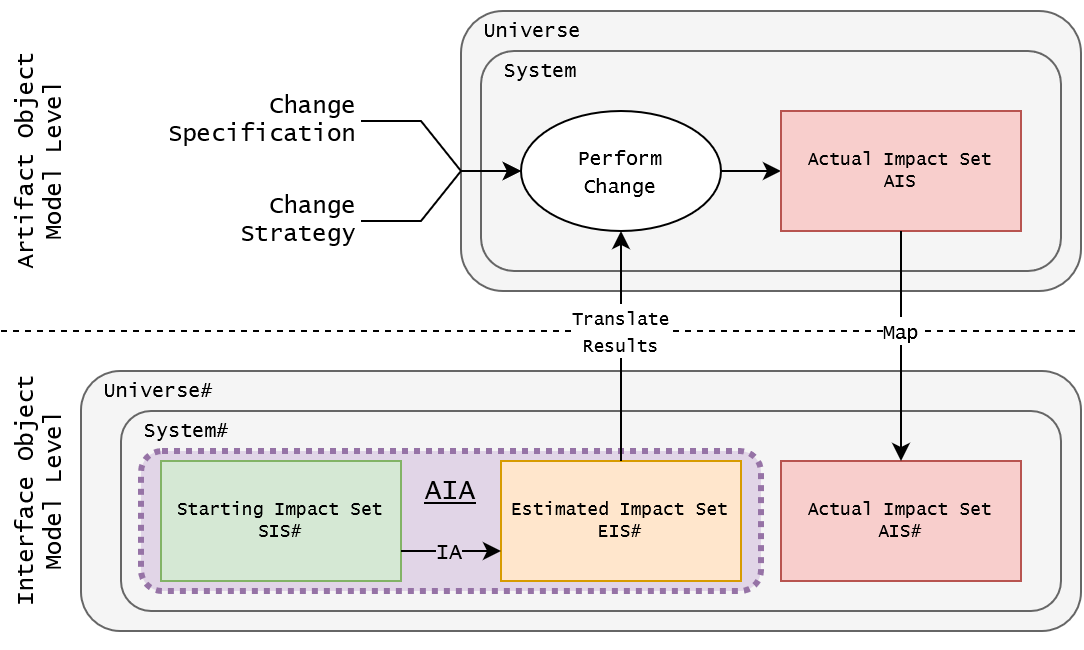
\includegraphics[width=1\linewidth]{gfx/IA35.drawio.png}
        \caption{Hauptmetriken der \ac{IA} Effektivität nach Arnold et al. \cite[296]{app_bohner}}
        [Eigene Darstellung]
        \label{fig:aia}
    \end{figure}
    
    \pagebreak
    \noindent
    Die definierten Mengen und Transformationen erlauben es im Folgenden Metriken zu definieren, welche Aussagen über die Genauigkeit und Effizienz des Verfahrens\footnote{der Impact-Analyse} treffen können.
    Hierbei entstehen drei sinnvolle Relationen, welche man im Folgenden betrachten kann:
    Die Relation zwischen der primären Anforderungsdefinition und der erarbeiteten Menge betroffener Entitäten\footnote{Bewertung der primären Änderungsdefinition}; das Verhältnis zwischen der erarbeiteten Menge betroffener Entitäten und dem Gesamtsystem\footnote{Bewertung der Eingrenzung}; und dem Abgleich der projizierten Menge betroffener Entitäten mit den eigentlich Betroffenen\footnote{Bewertung des Ergebnisses}.

    
\subsection{Bewertung der primären Änderungsdefinition}
    
    Die Bewertung der primären Änderungsdefinition beschäftigt sich mit dem Verhältnis von \acsfont{SIS\#} und \acsfont{EIS\#}. 
    Diese Metrik gibt Auskunft darüber, wie viele Entitäten -- die nicht durch die Änderungsdefinition vorgegeben waren -- durch die \ac{IA} als betroffen gekennzeichnet wurden.
    Definitionsgemäß\footnote{nach Arnold et al.} ist es jedoch nicht möglich, dass die Analyse primär markierte Entitäten aus der Schätzung ausschließt, weshalb dessen Menge immer eine Obermenge zur Menge der primären Änderungsdefinition darstellt.
    
    $$
        K = \dfrac{|\text{\acsfont{SIS\#}}|}{|\text{\acsfont{EIS\#}}|} \leq 1
    $$
    
    Im Rahmen der Bewertung der Impact-Analysen zu dem Thema dieser Arbeit gilt es als vorteilhaft, sowie die primäre Änderungsdefinition so genau wie möglich die Änderung des Systems beschreibt. 
    
    \begin{table}[H]
    \centering
    \hspace*{-1.75cm}
    \begin{tabular}{rc|c|>{\centering\arraybackslash}p{0.5\linewidth}|} 
        \cline{3-4} 
        & Fallabbildung & Bedingungen & Bewertung \\\cline{3-4}
        \vspace{-1.35em} \\ \cline{3-4}
            1&\begin{minipage}{0.25\textwidth}
                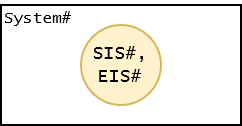
\includegraphics[width=\linewidth]{gfx/IA_1.drawio.png} 
            \end{minipage}
            &$\begin{array}{l}
                \scriptstyle EIS\# \;=\; SIS\#; \\
                \scriptstyle EIS\#,\; SIS\# \;\subseteq\; System\#
              \end{array}$ 
            &\begin{minipage}{0.5\textwidth} 
                \smaller
                \textit{Optimalfall}: Geschätzte Betroffenheit beschränkt sich auf die beschriebene Änderung.
            \end{minipage} 
            \\ \cline{3-4}
            2&\begin{minipage}{0.25\textwidth}
                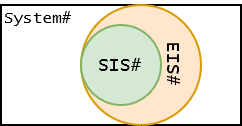
\includegraphics[width=\linewidth]{gfx/IA2.drawio.png} 
            \end{minipage}
            &$\begin{array}{l}
                \scriptstyle |EIS\#| \;>\; |SIS\#|; \\
                \scriptstyle SIS\# \;\subset\; EIS\#; \\
                \scriptstyle EIS\#,\; SIS\# \;\subseteq\; System\#
              \end{array}$ 
            & \begin{minipage}{0.5\textwidth} 
                \smaller
                \textit{Erwarteter Fall}: Die Analyse hat einige wenige Entitäten bestimmt, welche nicht in der primären Änderungsdefinition enthalten sind.
            \end{minipage} 
            \\ \cline{3-4}
            3&\begin{minipage}{0.25\textwidth}
                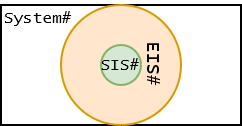
\includegraphics[width=\linewidth]{gfx/IA3.drawio.png} 
            \end{minipage}
            &$\begin{array}{l}
                \scriptstyle |EIS\#|\; \gg \; |SIS\#|; \\
                \scriptstyle SIS\# \;\subset\; EIS\#; \\
                \scriptstyle EIS\#,\; SIS\# \;\subseteq\; System\#
              \end{array}$ 
            & \begin{minipage}{0.5\textwidth}
                \smaller
                \textit{Suboptimal}: Eine große Diskrepanz zwischen \acsfont{SIS\#} und \acsfont{EIS\#} bedeutet einen höheren Arbeitsaufwand in späteren Schritten oder einer schlechten primären Änderungsdefinition.
            \end{minipage} 
            \\ \cline{3-4}
        \cline{3-4}
    \end{tabular}
    \caption{Mögliche \acsfont{SIS\#}/\acsfont{EIS\#} Abhängigkeiten nach Arnold et al. \cite[297]{app_bohner}}
    [Eigene Darstellungen]
    \label{tab:sis_eis}
\end{table}

    
% \begin{figure}[H]
%     \centering
%     \begin{tikzpicture}
%         \begin{axis}[
%             ybar stacked,
%         	bar width=15pt,
%         	nodes near coords,
%             enlargelimits=0.15,
%             legend style={at={(0.5,-0.20)},
%               anchor=north,legend columns=-1},
%             ylabel={\#participants},
%             symbolic x coords={Erwünscht, Erwartet, Ziel},
%             xtick=data,
%             x tick label style={rotate=45,anchor=east},
%             ]
%         \addplot+[ybar] plot coordinates {(Erwünscht,1) (Erwartet,0.05) (Ziel,0.2)};
%         \addplot+[ybar] plot coordinates {(Erwünscht,0) (Erwartet,0.4) (Ziel,0.6)};
%         \addplot+[ybar] plot coordinates {(Erwünscht,0) (Erwartet,0.55) (Ziel,0.1)};
%         \legend{\strut K = 1, \strut 0.7 < K < 1, \strut K $\leq$ 0.7}
%         \end{axis}
%     \end{tikzpicture}
%     \caption{Caption}
%     \label{fig:enter-label}
% \end{figure}

\pagebreak
\subsection{Bewertung der Eingrenzung}
    
    Im Weiteren kann bewertet werden, wie gut die Ergebnismenge eingeschränkt ist.
    Bei der Natur einiger Änderungen kann diese Metrik auch eine Aussage darüber treffen, wie Änderungen innerhalb von Abhängigkeiten propagiert werden. 
    So beschreibt ein hoher Wert der Metrik entweder ein stark vernetztes System, welches Änderungen leicht propagiert oder eine \ac{IA}, welche viele abhängige Entitäten in die Ergebnismenge mit einschließt.
    Je genauer die \ac{IA} die Ergebnismenge einschränken kann, desto nützlicher ist das Ergebnis für den weiteren Prozess, da der Arbeitsaufwand so gering wie möglich bleibt. 
    
    $$
        J = \dfrac{|\text{\acsfont{EIS\#}}|}{|\text{System\#}|} \leq 1
    $$
    
    Für die Prozesse der Nachweisführung regulativer Anforderungen ist diese Metrik direkt mit dem Arbeitsaufwand des Änderungsprozesses verknüpft.
    Es gilt also im für die Bewertung einer \ac{IA} als vorteilhaft, sowie Änderungen möglichst präzise auf die betroffenen Anfoderungen eingegrenzt werden kann, da hierdurch Effizienz der Nachweisführungsprozesse verbessert werden kann.
    
    
\begin{table}[H]
    \centering
    \hspace*{-1.75cm}
    \begin{tabular}{rc|c|>{\centering\arraybackslash}p{0.5\linewidth}|} 
        \cline{3-4} 
        & Fallabbildung & Bedingungen & Bewertung \\\cline{3-4}
        \vspace{-1.35em} \\ \cline{3-4}
            1&\begin{minipage}{0.25\textwidth}
                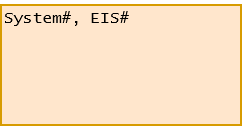
\includegraphics[width=\linewidth]{gfx/IA21.drawio.png} 
            \end{minipage}
            &$\begin{array}{l}
                \scriptstyle EIS\# \;=\; Sys\#; \\
              \end{array}$ 
            &\begin{minipage}{0.5\textwidth} 
                \smaller
                \textit{Standardfall}: Keine große Aussage für \ac{IA} kann jedoch ein System mit sehr vielen Abhängigkeiten identifizieren.
            \end{minipage} 
            \\ \cline{3-4}
            2&\begin{minipage}{0.25\textwidth}
                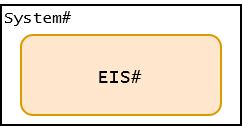
\includegraphics[width=\linewidth]{gfx/IA22.drawio.png} 
            \end{minipage}
            &$\begin{array}{l}
                \scriptstyle |System\#| \;>\; |EIS\#|; \\
                \scriptstyle EIS\# \;\subset\; System\# \\
              \end{array}$ 
            & \begin{minipage}{0.5\textwidth} 
                \smaller
                \textit{Verbesserter Fall}: Die geschätzte Änderung betrifft nicht das gesamte System und kann genauer definiert werden.
            \end{minipage} 
            \\ \cline{3-4}
            3&\begin{minipage}{0.25\textwidth}
                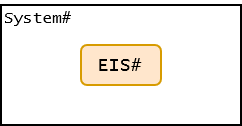
\includegraphics[width=\linewidth]{gfx/IA23.drawio.png} 
            \end{minipage}
            &$\begin{array}{l}
                \scriptstyle |System\#|\; \gg \; |EIS\#|; \\
                \scriptstyle EIS\# \;\subset\; System\# \\
              \end{array}$ 
            & \begin{minipage}{0.5\textwidth}
                \smaller
                \textit{Optimalfall}: Geschätzte Änderung beschränkt sich auf eine relativ kleine Untermenge des Systems.
            \end{minipage} 
            \\ \cline{3-4}
        \cline{3-4}
    \end{tabular}
    \caption{Mögliche \acsfont{EIS\#}/\acsfont{System\#} Abhängigkeiten nach Arnold et al. \cite[297]{app_bohner}}
    [Eigene Darstellungen]
    \label{tab:eis_sys}
\end{table}


\subsection{Bewertung des Ergebnisses}
    
    Die letzte Metrik, welche verwendet werden kann, um die \ac{IA} zu bewerten, ist der Vergleich der ermittelten Menge mit der tatsächlich betroffenen Menge.
    Die beiden Mengen\footnote{\acsfont{EIS\#} und \acsfont{AIS\#}} stellen hierbei gegenseitige keine Teil- oder Obermengen dar, weshalb die Metrik nicht begrenzt ist.
    Eine zweite Metrik gibt an, wie groß die Schnittmenge der beiden Mengen ist, um auszuschließen, dass die Mengen keine Elemente teilen (siehe Fall 7, Tabelle \ref{tab:eis_ais}). 
    
    $$
        H = \dfrac{|\text{\acsfont{AIS\#}}|}{|\text{\acsfont{EIS\#}}|}; \quad
        % M = \dfrac{|\text{\acsfont{EIS\#}}|}{|\text{\acsfont{AIS\#}}|}; \quad
        N = |\acsfont{AIS\#} \cap \acsfont{EIS\#}|
    $$
    
    Der Optimalfall für die Nachweisführungsprozesse der Flugsicherung sollte einer der sicheren Fälle (Fälle 1-3, Tabelle \ref{tab:eis_ais}) umfassen, da diese Fälle die Vollständigkeit der Nachweisführung nicht gefährden.
    Weiter beläuft sich die Differenz der Mengen im Optimalfall gegen null, da hierdurch der manuelle Arbeitsaufwand -- Änderungen als nicht relevant zu markieren -- so gering wie möglich ausfällt.
    \bigskip
    
    
\begin{table}[H]
    \centering
    \hspace*{-1.75cm}
    \begin{tabular}{rc|c|>{\centering\arraybackslash}p{0.5\linewidth}|} 
        \cline{3-4} 
        & Fallabbildung & Bedingungen & Bewertung \\\cline{3-4}
        \vspace{-1.35em} \\ \cline{3-4}
            1 & \begin{minipage}{0.25\textwidth}
                    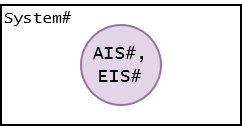
\includegraphics[width=\linewidth]{gfx/IA41.drawio.png} 
                \end{minipage}
                &$\begin{array}{l}
                    \scriptstyle EIS\# \;=\; AIS\#; \\
                    \scriptstyle EIS\# \;\subset\; System\# \\
                  \end{array}$ 
                &\begin{minipage}{0.5\textwidth} 
                    \smaller
                    \textit{Optimales Ergebnis}: Geschätzter Impact stimmt mit \acsfont{AIS\#} überein. Spricht für eine sehr hilfreiche \ac{IA}.
                \end{minipage} 
            \\ \cline{3-4}
            2 & \begin{minipage}{0.25\textwidth}
                    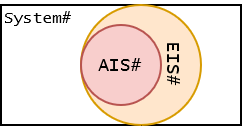
\includegraphics[width=\linewidth]{gfx/IA42.drawio.png} 
                \end{minipage}
                &$\begin{array}{l}
                    \scriptstyle |EIS\#| \;>\; |AIS\#|; \\
                    \scriptstyle AIS\# \;\subset\; EIS\#; \\
                    \scriptstyle EIS\# \;\subseteq\; System\# \\
                  \end{array}$ 
                & \begin{minipage}{0.5\textwidth} 
                    \smaller
                    \textit{Gutes sicheres Ergebnis}: Alle eingetroffenen Änderungen wurden richtig eingeschätzt und die Differenz der Mengen ist nicht sehr groß.
                \end{minipage} 
            \\ \cline{3-4}
            3 & \begin{minipage}{0.25\textwidth}
                    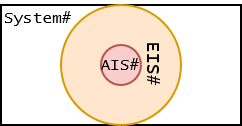
\includegraphics[width=\linewidth]{gfx/IA43.drawio.png} 
                \end{minipage}
                &$\begin{array}{l}
                    \scriptstyle |EIS\#| \;\gg\; |AIS\#|; \\
                    \scriptstyle AIS\# \;\subset\; EIS\#; \\
                    \scriptstyle EIS\# \;\subseteq\; System\# \\
                  \end{array}$ 
                & \begin{minipage}{0.5\textwidth}
                    \smaller
                    \textit{Schwaches sicheres Ergebnis}: Alle Änderungen wurden richtig eingeschätzt, jedoch ist die Differenz der Mengen sehr groß und es wurde viele weitere Entitäten falsch markiert.
                \end{minipage} 
            \\ \cline{3-4}
            4 & \begin{minipage}{0.25\textwidth}
                    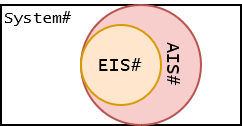
\includegraphics[width=\linewidth]{gfx/IA44.drawio.png} 
                \end{minipage}
                &$\begin{array}{l}
                    \scriptstyle |AIS\#| \;>\; |EIS\#|; \\
                    \scriptstyle EIS\# \;\subset\; AIS\#; \\
                    \scriptstyle AIS\# \;\subseteq\; System\# \\
                  \end{array}$ 
                & \begin{minipage}{0.5\textwidth}
                    \smaller
                    \textit{Unsicheres Ergebnis}: Die Abschätzung verfehlt die komplette Abdeckung aller betroffenen Änderungen.
                \end{minipage} 
            \\ \cline{3-4}
            5 & \begin{minipage}{0.25\textwidth}
                    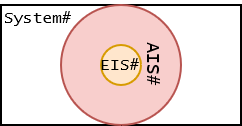
\includegraphics[width=\linewidth]{gfx/IA45.drawio.png} 
                \end{minipage}
                &$\begin{array}{l}
                    \scriptstyle |AIS\#| \;\gg\; |EIS\#|; \\
                    \scriptstyle EIS\# \;\subset\; AIS\#; \\
                    \scriptstyle AIS\# \;\subseteq\; System\# \\
                  \end{array}$ 
                & \begin{minipage}{0.5\textwidth}
                    \smaller
                    \textit{Stark unsicheres Ergebnis}: Die Abschätzung verfehlt die betroffenen Änderungen sehr. Die große Diskrepanz bedarf weiterer Arbeit zum Erschließen der \acsfont{AIS\#}.
                \end{minipage} 
            \\ \cline{3-4}
            6 & \begin{minipage}{0.25\textwidth}
                    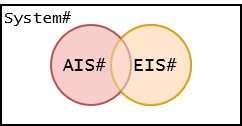
\includegraphics[width=\linewidth]{gfx/IA46.drawio.png} 
                \end{minipage}
                &$\begin{array}{l}
                    \scriptstyle |AIS\# \;\cap\; EIS\#|\; > \; 0; \\
                    \scriptstyle EIS\# \;\neq\; AIS\#; \\
                    \scriptstyle EIS\# \;\subseteq\; System\# \\
                  \end{array}$ 
                & \begin{minipage}{0.5\textwidth}
                    \smaller
                    \textit{Verfehltes Ergebnis}: Die Abschätzung verfehlt die komplette Abdeckung aller betroffenen Änderungen und beinhaltet nicht betroffene Entitäten.
                \end{minipage} 
            \\ \cline{3-4}
            7 & \begin{minipage}{0.25\textwidth}
                    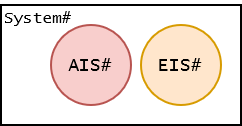
\includegraphics[width=\linewidth]{gfx/IA47.drawio.png} 
                \end{minipage}
                &$\begin{array}{l}
                    \scriptstyle |AIS\# \;\cap\; EIS\#|\; = \; 0; \\
                    \scriptstyle EIS\# \;\subset\; System\#; \\
                  \end{array}$ 
                & \begin{minipage}{0.5\textwidth}
                    \smaller
                    \textit{Stark verfehltes Ergebnis}: Extremere Version von Fall 6.
                \end{minipage} 
            \\ \cline{3-4}
        \cline{3-4}
    \end{tabular}
    \caption{Mögliche \acsfont{AIS\#}/\acsfont{EIS\#} Abhängigkeiten nach Arnold et al. \cite[299]{app_bohner}}
    [Eigene Darstellungen]
    \label{tab:eis_ais}
\end{table}


\chapter{Datenquelle 1: Europäische Verordnungen und EurLex}

\begin{quote}
\textcolor{red}{Einführung in die EU VOs als Datenquelle. Zuerst thematisch in die Arbeitsweise und anschließenden digital, in die Möglichkeiten auf die Daten zuzugreifen.
Zuerst kurze Einführung, warum EU (naheliegend)}
\end{quote}

    \section{Europäische Verordnungen}
        \subsection{Beteiligte Organisationen}
    
            \pagebreak    
        
            
\begin{quote}
\textcolor{green}{Diese Seite auch}
\end{quote}
            \pagebreak    
        \subsection{Ordentliches Gesetzgebungsverfahren}
            \pagebreak    
        
        \subsection{Konsolidierungen von Verordnungen / Lifecycle}
            \pagebreak    
        

    \section{OpenData in der Europäischen Union}

Die Jahre 2003 wurde durch die EU die sogenannte \textit{PSI-Richtlinie} (Re-use of Public Sector Information 2003/98/EG) veröffentlicht, welche einen möglichst einfachen, unbürokratischen und allgemeinen Zugriff auf Informationen ermöglichen soll.
Die Richtlinie wurde im November 2005 auf den Geltungsbereich des EWR ausgeweitet\cite{2005D0105} und im Dezember 2006 durch das \textit{Informationsweiterverwendungsgesetz(IWG)} in nationales Recht umgesetzt.
Auf Basis von erheblichen Änderungen eben dieser Richtlinie im Verlaufe der Zeit entschied sich die Kommission für eine Neufassung der Richtlinie, welche im Jahr 2019 erschien und die alte Richtlinie in seiner Gültigkeit ablöst. \cite[Prä. Abs. 1ff.]{2003L0098}



        
        % \pagebreak
        \subsection{OpenData Project / Vision}

Um die Bemühungen der definierten Initiative für Open-Data weiter zu unterstützen, wurde im Folgenden unter anderem wissenschaftliche Projekte und Arbeiten finanziert.
Beispielsweise 



        
        \pagebreak
        \subsection{EU Cellar Plattform}

        \subsubsection{Motivation}
        
Gestützt durch die PSI-Richtlinie, dem Strategiedokument \textit{Europa 2020} für u.a. der ,,Entwicklung einer auf Wissen und Entwicklung gestützten Wirtschaft`` und dem Arbeitsvertrag der Europäischen Union(AEUV), insbesondere Art. 249, beschließt die EU im Jahre 2011 auch die Weiterverwendung der eigenen Kommissionsdokumente.\cite[Prä. 1]{2011D0833}

        \subsubsection{Umsetzung}

Nach dieser Richtlinie legt sich die Kommission fest, ein Datenportal einzurichten, welches einen zentralen Zugang zu ihren strukturierten Daten ermöglicht und folglich die Verknüpfung und Weiterverwendung für kommerzielle oder nichtkommerzielle Zwecke zu erleichtern. \cite[Art. 5]{2011D0833}
Die hieraus entstandene Cellar Plattform ist ein öffentliches semantisches Repository des \textit{Amts für Veröffentlichung der EU} (OP), welche unter anderem EUR-Lex\footnote{\href{https://eur-lex.europa.eu/homepage.html?locale=de}{https://eur-lex.europa.eu/}}, als digitales Zugangsportal zu europäischem Recht, als auch eine eigene Plattform\footnote{ehemals EU-Bookshop: \href{https://bookshop.europa.eu/}{https://bookshop.europa.eu/}} zur Publikation von weiteren informativen wie wissenschaftlichen Dokumenten ermöglicht.
Die Struktur der Daten basiert auf \textit{Semantic Technologies} und ermöglicht es, Daten auf Basis von definierten Standards weiterzunutzen und zu teilen. 
\cite[5]{eu_cellar}

        \subsubsection{Umsetzung}

Weiter werden Dokumente auch, soweit sinnvoll und nicht mit einem unverhältnismäßigen Mehraufwand verbunden, in einem maschinenlesbaren Format zur Verfügung gestellt \cite[Art. 8 Abs. 1f]{2011D0833}







        % \subsubsection{Unterschiedliche Formate etc}
        \pagebreak
    
    \section{Integration in die Analyse / Prozesse}
    
\begin{quote}
\textcolor{green}{1-2 Seiten}
\end{quote}

\subsection{Übertrag auf das erarbeitete Datenmodell}
\pagebreak
\chapter{Datenquelle 2: EASA und Easy Access Rules}

    \section{European Union Aviation Safety Agency}

% \begin{quote}
% \textcolor{red}{Einführung zur EASA. Neue Position und Bedeutung für den Prozess. Was sind Easy Access Rules und welche Bedeutung haben sie für uns. Hard law / Soft law. Added benefit durch AMC/GM}
% \end{quote}
% \begin{quote}
% \textcolor{green}{1-2 Seiten}
% \end{quote}

Nach dem informellen Zusammenschluss paneuropäischer nationaler Luftfahrtbehörden (\acs{NAA}), zwecks der Standardisierung von Flugzeugzertifizierungsprozessen ab 1970\footnote{\acf{JAA}} erkannten \ac{EU} Initiativen 1996 bereits den Bedarf einer zentralen europäischen Luftfahrtbehörde.
Im Jahre 1990 definierte die Kommission Ziele an eine ,,Harmonisierung der technischen Vorschriften und Verfahren für Zivilluftfahrzeug[!]``\cite{kom_90_442}, welche unter anderem anregten: 

\begin{quote}
    ,,Dieser Ansatz sollte langfristig zur Schaffung einer einheitlichen Europäischen Luftfahrtbehörde führen, wodurch eine völlige Harmonisierung der Sicherheitsnormen und deren konsequente Durchführung sichergestellt wären.``\footnote{Im Rahmen dieses Vorschlags war die Schaffung einer solchen Behörde explizit von dem Rahmen des Dokuments ausgenommen (siehe gleicher Absatz)} \cite[Begr. Art. 7 Abs. 2]{kom_90_442}
\end{quote}
Auf Basis dieser Bemühungen wurde die \acf{EASA}\footnote{Zunächst definiert als European Aviation Safety Authority \cite[2]{easa_framework}} im Jahre 2002 durch die Verordnung \vo{VO}{EG}{1592/2002} offiziell als Einrichtung der \ac{EU} gegründet und würde ein Jahr später ihre zuvor definierte Arbeit aufnehmen.
Nach dieser Definition sollte die \ac{EASA} zunächst die Zusammenarbeit der europäischen \acsp{NAA} koordinieren und dessen Meinungen im Umfeld der \ac{EU}-Organe repräsentieren. 
\cite{easa_coman2018}

\subsubsection{Aufgaben der EASA}

Im Rahmen der Verordnungen \vo{VO}{EG}{216/2008}\textdagger{} und \vo{VO}{EU}{2018/1139} wurden die Aufgaben


        
        % \subsubsection{Bedeutung nach VO 2023/1768ff.}
        
        \pagebreak

        \subsection{Annehmbare Nachweisverfahren}

        Die \ac{EASA} ist nach der Anforderung \textsf{ATM/ANS.AR.A.015.a} angehalten, annehmbare Nachweisverfahren (engl. Accepted Means of Compliance (AMC)) zu entwickeln, welche zur Bewertung der Compliance herangezogen werden können und dessen Abdeckung eine vollständige Abdeckung der zugrundeliegenden einschlägigen Verordnung garantiert. 
        \cite[Anh. II]{2017R0373}


    \subsubsection{Alternative Nachweisverfahren}
        
        

        \subsection{Guidance Material}

\pagebreak

        \subsection{Easy Access Rules}

\subsubsection{Definition nach FRBR}

Im Rahmen der behandelten Definitionen aus der Studie zu funktionalen Anforderungen bibliografischer Datensätze \acs{FRBR} (siehe \ref{frbr}) bilden die \textit{Easy Access Rules} eine weitere \textit{Manifestation} des bestehenden \textit{Werkes} der referenzierten, abgedeckten Verordnung.
Auch wenn die \ac{EAR} den Umfang bestehender \textit{Manifestationen} inhaltlich um \textit{Annehmbare Nachweisverfahren} und \textit{Guidance Material} erweitern, so ändern sie nicht 

        \pagebreak
    \section{EASA eRules Plattform}

    Die \ac{EASA} eRules Plattform ist ,,einheitliche, einfach zugängliche, online Datenbank für alle in der Luftfahrt anwendbaren Regeln für Stakeholder im europäischen Luftraum``.
    \cite[5]{easa_xml_doc}

    Als ein Produkt dieser Plattform werden die sogenannten Easy Access Rules definiert und bis dato (24.6.22) in zwei Formaten veröffentlicht. 

    
Am 26. Januar 2023 veröffentlichte die EASA die Entscheidung, Easy Access Rules fortan auch in einem maschinenlesbaren XML Format Endnutzern bereitzustellen. \cite{easa_xml_publication}


\subsection{Informationsarchitektur}
\label{ch:easa_arch}

    Im Rahmen der eRules Plattform und des maschinenlesbaren \ac{XML} Formates, werden Inhalte in kleine sogenannte ,,Topics`` unterteilt.
    Ein Topic repräsentiert eine \ac{EU} Durchführungsbestimmung (siehe \ref{ch:ir}); eine \ac{EU} Delegierte Bestimmung; ein Annehmbares Nachweisverfahren der \ac{EASA}; \ac{EASA} Guidance Material; oder sog. \ac{EASA} \acf{CertS}\footnote{(CS) wegen Überschneidung mit \acf{CS} geändert}. \cite[S. 5f]{easa_xml_doc}
    
Topics werden repräsentativ ihrer konzeptuellen Beziehungen zwischen den unterschiedlichen Topics in der baumartigen Struktur abgebildet.
Hierbei werden Topics, welche Verordnungen oder \ac{CertS} abbilden meist auf einem strukturell höheren Level und alle diesem zugeordneten Topics wie. \acsp{AMC}, \acsp{GM}, oder anderen Gesetzesgrundlagen dargestellt.


        
        \subsubsection{Publikationsformat}

    Die für die Publikation der maschinenlesbaren Dokumente wählte die \ac{EASA} die von \acf{MS} etablierte und standardisierte \acf{OPC}\footnote{\acs{ECMA}-376, ISO/IEC 29500-2}.
    Dieser Standard ist Teil der Familie an \ac{XML} Schemata, welche gemeinsam als \acf{OOXML} bezeichnet werden\footnote{ ISO/IEC 29500} und \ac{XML} Semantiken für Textverarbeitungs-, Tabellen\-kal\-ku\-lations- und Präsentationsdokumente -- oder hiermit konformen Dokumenten -- bereitstellen. 
    \cite[vii]{easa_opc_iso} 
    Die Besonderheit dieses Formates ist es, dass das Gesamtdokument in kleineren Parts\footnote{gemäß 6.2 ISO/IEC 29500-2 \cite{easa_opc_iso}} strukturiert wird, welche nach der Definition der \ac{OPC} -- ähnlich wie ein Archiv -- in ein Gesamtdokument zusammengefasst werden.
    Hierauf basierende Standards, wie \ac{OOXML}, definieren meist nur die Struktur einzelner Parts, was eine konforme Erweiterung des Gesamtdokumentes durch weitere Parts problemlos ermöglicht.   
    Dies bedeutet unter anderem, dass valide Dokumente Teil von größeren Gesamtdokumentes sein können, wessen weitere Parts keinen Einfluss auf dessen Benutzung als konformes Open Office-Dokument nehmen.
    Genau von dieser Eigenschaft hat die \ac{EASA} Gebrauch gemacht und ihre Informationen auf zwei Arten in das Gesamtdokument integriert:

            \subsubsection{Anforderungsinhalte}

    Inhalte von Topics werden unter Release 1.0.0 der eRules \ac{XML} Spezifikation als ,,opaque data structure`` angesehen.
    Dies bedeutet, dass im Zug dieses Releases keine inhaltliche Struktur der Inhalte der Topics definiert wurde.
    Es bleibt jedoch den Anwender:innen überlassen, Implementationen auf die Angaben innerhalb des beschriebenen \acs{OOXML} Formates zu stützen.
    \cite[6]{easa_xml_doc}

    % \medskip
    Nach diesem Standard sind die textuellen Inhalte der einzelnen Topics Teil des Textverarbeitungsdokumentes\footnote{Part Name: "\textit{/word/document.xml}"} und lassen sich damit auch über eine grafische Textbearbeitungsoberfläche (bspw. \ac{MS} Word) einsehen und bearbeiten.
    Hierbei werden Textinhalte des Dokumentes so strukturiert, dass die einzelnen Entitäten voneinander isoliert und über eine -- innerhalb des Dokumentes -- lokal einzigartige ID, eindeutig identifizierbar gemacht werden.
    So können die Inhalte bei Bedarf beliebig bearbeitet werden, ohne die Struktur der Topics oder die Integrität anderer strukturellen Verweise zu gefährden.
            % Außerdem ist es so möglich, Einträge in den Metadaten auf die entsprechenden Anforderungsinhalte verweisen zu lassen. 

            \subsubsection{Metadaten}

    % Zusätzlich zu den Inhalten ermöglicht es der \ac{OOXML} Standard, weitere Parts an das Textdokument anzuhängen.
    Die \ac{EASA} nutzt zusätzlich die Möglichkeit, konforme \ac{OOXML} um eigene Parts zu erweitern, um das inhaltliche Dokument mit Metadaten der einzelnen Topics, auf Basis des internen \ac{EASA} \ac{CCMS}, zu bereichern.
    Diese Metadaten enthalten interne Informationen zu der Struktur des Dokumentes und den einzelnen Anforderungen und stehen dem Endnutzer in Form eines \ac{OPC} Parts  zur Verfügung.
    Dessen Struktur beruht auf einem eigenen \ac{XML} Schema, welches in der entsprechenden Dokumentation der \ac{EASA} definiert ist.

\pagebreak
\subsection{Analyse der Metadaten}
\label{ch:easa_anal}

    Die für diese Analyse relevanten Attribute, welche Metadaten der oben definierten Topics beschreiben, werden im Rahmen der Dokumentation unter der Gruppe ,,\textsf{topic-metadata}``\footnote{\ac{XSL} Attribute Group} festgehalten.
    Diese Gruppe beinhaltet die im Folgenden analysierte Attribute.\footnote{Alle beschriebenen Attribute werden durch den Typ String ohne jegliche Einschränkungen abgebildet und im Folgenden durch ,,[AttributName] Attribut`` oder -- gemäß dem XPath Standard -- ,,@[AttributName]`` referenziert} \cite[9]{easa_xml_schema}

    \subsubsection{ERulesId}

Die \textit{ERulesId} stellt eine -- über alle publizierten Dokumente hinweg -- einzigartige Kennung eines jeden Topics dar.
Dies ermöglicht eine einfache, einheitliche Referenzierung von Topics unabhängig von deren zugehörigem Dokument.
Die \ac{EASA} garantiert diesbezüglich, dass die Id über den gesamten Lifecycle des Topics unveränderlich sind. \cite[17]{easa_xml_doc}

In Bezug auf die Impactanalyse, bietet dieses Attribut einen großen Vorteil, da die definierten Anforderungen an eine \textit{Eindeutige Kennung} (vgl. \ref{model_anforderungen}) bereits für alle Topics der \ac{EASA}\footnote{Darunter, durch \ac{IR}, auch \atmans Anforderungen} erfüllt sind.
% \medskip
\begin{quote}
Beispiel:
\textsf{ERulesId="{}ERULES-1891294191-107"}
\end{quote}

% A unique identifier attribute for every topic in the exported XML file, which allows the unique identification of a topic across all the exported XML files from EASA. The ERulesId value is unchanged: • from publication to publication, everywhere the topic is reused; and • from version to version, throughout the entire life cycle of the topic.  
    
    \subsubsection{Domain / Activity Type}

Die \textit{Domain} und der \textit{Activity Type} eines Topics bezeichnen dessen Aufgabenbereich sowie die technische Beschreibung der darin vollbrachten Aufgabe \cite[S. 18]{easa_xml_doc}.
Im Umfang der nach \vo{VO}{EU}{2018/1139} i.V.m. \vo{VO}{EU}{628/2013} definierten Aufgabenbereiche kann in unserem Falle immer die \textit{Domain} \atmans angenommen werden.

Mögliche Werte des \textit{ActivityType}-Attributs beinhalten u.a.\footnote{Nicht holistische Liste an Beispielen \cite[vgl.][S.18 -- 19]{easa_xml_doc}} die unter \atmans definierten Aufgaben (siehe \ref{beg:atmans}).
Sie geben in der folgenden Analyse Auskunft darüber, für welche \atmans Ausrüstungen die Topics eine Relevanz aufweisen.
Dies kann u.a. genutzt werden, um die Relevanz neuer Anforderungen zu ermitteln oder irrelevante Anforderungen im Nachweisführungsprozess anderer Ausrüstungen auszuschließen.  

\begin{quote}
    Beispiel:
    \textsf{ActivityType="Meteorological Services (MET)"}
\end{quote}
   
    \subsubsection{AircraftCategory / AircraftUse / RegistryState}

Die Attribute \textit{AircraftCategory}, \textit{AircraftUse} und \textit{RegistryState} beziehen sich auf die Klassifizierung und Zuordnung von Anforderungen an Flugzeuge und haben für \atmans Equipment kein Gewicht\footnote{Eine vorangehende Analyse hat ergeben, dass diese Attribute in den \atmans Dokumenten nicht verwendet werden}. \cite[20, 21, 26]{easa_xml_doc}
    
    \subsubsection{AmendedBy}

Im Falle von Änderungen des \textit{Topics} referenziert dieses Attribut die lokale Konsolidierung der \ac{EAR}
\cite[21]{easa_xml_doc}.
Nach deren Publikation unbearbeitete \textit{Topics} führen den Wert \textsf{"{}Initial issue;"}

\begin{quote}
    Beispiel:
    \textsf{AmendedBy="{}Amendment 1;"}\footnote{Die Kennung der Änderung bezieht sich ausschließlich auf die aktuelle \ac{EAR}}
\end{quote}
    
    \subsubsection{ApplicabilityDate / EntryIntoForceDate }

Die Attribute \textit{Applicability-} und \textit{EntryIntoForceDate} beschreiben im Falle von Topics, welche sich auf Durchführungsbestimmungen beziehen, den entsprechenden zeitlichen Rahmen von deren Gültigkeit.
Das \textit{ApplicabilityDate} repräsentiert dabei -- unabhängig von dem juristischen Wortlaut -- den letzten Tag der Übergangsperiode. 
Das \textit{EntryIntoForceDate} hingegen repräsentiert das offizielle Inkrafttreten rechtlicher Durchführungsbestimmungen, nach welcher die rechtliche Bindung der in dem Topic abgebildeten Anforderung beginnt.
\cite[21]{easa_xml_doc}
Mangels rechtliche Bindung verfügen Topics in Bezug auf \acsp{AMC} oder \ac{GM} nicht über diese Attribute.\footnote{Strukturell sind alle Topics gleich, der Wert bleibt lediglich leer}
    
    \subsubsection{EquivalentForeignRegulation}

Das Attribut \textit{EquivalentForeignRegulation} äquivalente Regularien von nicht \ac{EU} Mitgliedstaaten.
Diese Informationen werden -- nach Angaben der \ac{EASA} -- hauptsächlich zum Angleichen von Designstandards von Flugzeugdesigns genutzt \cite[22]{easa_xml_doc}, finden nach eigener Auswertung aber auch im \atmans Sektor Anwendung, um bspw. international gemeinschaftliche Nachweisverfahren zur Luftdatenverarbeitung zu etablieren (siehe Beispiel).

\begin{quote}
    Beispiel:
    \textsf{EquivalentForeignRegulation="{}AC No: 20-153B;"}\footnote{Referenziert \ac{FAA}: \ac{AC} 20-153B - ,,Acceptance of Aeronautical Data Processes and Associated Databases``}$^,$\footnote{Semikolon beschreibt mögliche Auflistung mehrerer (durch Semikola getrennte) Einträge }
\end{quote}

    \subsubsection{ICAOReference}

Verweist auf -- im Rahmen des \textit{Topics} -- relevante \ac{ICAO} \acp{SARP}. 
\cite[23]{easa_xml_doc}

\begin{quote}
    Beispiel:
    \textsf{ICAOReference="{}Annex 11; Annex 19;"}
\end{quote}
    
    \subsubsection{Keywords}

    Die Verwendung des \textit{Keyword} Attributs ist nach der offiziellen Dokumentation nicht genau festgelegt.
    Es wird verwendet, um weitere Metadaten anzuhängen oder eine Kategorisierung anhand einzelner Schlüsselwörter umzusetzen.
\cite[23--26]{easa_xml_doc}
    \begin{quote}
    Beispiel:
    \textsf{Keywords="{}Safety measures; safety tracking"}
\end{quote}

    \subsubsection{RegulatedEntity}

Die regulierte juristische Person (\textit{regulated entity}) definiert, an wen die -- im \textit{Topic} definierte -- Anforderung gerichtet ist und wer diese im gleichen Zug zu erfüllen hat.
Diese \textit{Entities} beschreiben entweder Stakeholder:innen der Luftfahrtindustrie oder der zuständigen Behörde\footnote{hier \ac{EASA}} \cite[26]{easa_xml_doc}.

Im Rahmen der \atmans Anforderungen kann dieses Attribut auch die Anbieter der definierten \atmans Dienste definieren.
Diese Informationen können so eine sehr gute Abbildung erzeugen, welche Bereiche im \atmans Sektor von entsprechende \textit{Topics} reguliert werden.  
    \begin{quote}
    Beispiel:
    \textsf{RegulatedEntity="{}ATS provider; ANS provider;"}
\end{quote}

    
    \subsubsection{Regulatory Source}

Die Funktion dieses Attribut beschreibt -- analog zur Definition aus \ref{model_anforderungen} -- die Regulatorische Quelle der Durchführungsrichtlinie.
Im Genaueren definiert die \textit{Regulatory Source} den Rechtsakt, welcher das \textit{Topic} eingeführt\footnote{i.V.m. \textit{@AmendedBy} \textsf{"{}InitialIssue"} / "FurtherIssue"} oder zuletzt konsolidiert\footnote{i.V.m. \textit{@AmendedBy} \textsf{"{}Amendment [...]"}} hat \cite[27]{easa_xml_doc}. 

    \begin{quote}
    Beispiel:
    \textsf{RegulatorySource="{}Regulation (EU) 2021/1338"}
\end{quote}

    \subsubsection{Regulatory Subject}

Der Regulierungsgegenstand (\textit{Regulatory Subject}) referenziert das relevante Material des \textit{Topics}. 
Dieses beschreibt den strukturellen Teil, in welchem es durch das Amtsblatt oder die \ac{EASA} Website publiziert wurde \cite[28]{easa_xml_doc}.
Im Falle der \atmans Anforderungen aus der \vo{DVO}{EU}{2017/373} bezieht sich dieses Attribut entweder auf den eigenen Verordnungstext\footnote{Wert ,,cover regulation``} oder einer der, in den Anhängen, definierten ,,Parts``.
\begin{quote}
    Beispiel:
    \textsf{RegulatorySubject="Part-ATS;"}
\end{quote}


    \subsubsection{TechnicalSubjectMatter / EASACategory}

Referenziert zumeist technische Systeme von Flughäfen oder \ac{EASA} Kategorisierungen von Landebahnen und findet für \atmans Equipment keine Anwendung. \cite[28--29, 31]{easa_xml_doc} 

   \pagebreak
    \subsubsection{TypeOfContent}

Das \textit{TypeOfContent} Attribut definiert den Typ und die Funktion des \textit{Topics}.
Neben den oben definierten Typen von \textit{Topics} spezifiziert das Attribut im Falle von untergeordneten Topics auch den Typen des nächsthöheren, referenzierten \textit{Topics} 
(bspw.: ,,AMC to IR``\footnote{Annehmbare Nachweisverfahren von Anforderungen}, ,,GM to AMC``\footnote{Anleitungen zu Annehmbaren Nachweisverfahren}, ,,GM to IR``\footnote{Anleitungen zu Anfoderungen})

    \begin{quote}
    Beispiel:
    \textsf{TypeOfContent=\\"{}AMC to IR (Acceptable means of compliance to implementing rule);"}
\end{quote}

    
    \subsubsection{ParentIR}

    Das \textit{ParentIR} Attribut referenziert\footnote{durch das Titel-Attribut (@source-title) des anderen Topics (nicht Teil von topic-metadata)} das jeweils -- nach der Table Of Content (ToC) Hierarchie -- direkt-übergeordnete \textit{Topic}.
    Befindet sich das Topic bereits auf der obersten Ebene, bleibt dieses Feld leer.
    Diese Eigenschaft ermöglicht es, die Position eines \textit{Topics} innerhalb der Hierarchie zu bestimmen und im Falle eines \ac{AMC} oder \ac{GM} \textit{Topics} die jeweils abgedeckte Grundlage zu bestimmen.
    Wie in der Abbildung \ref{fig:parent_ir} dargestellt, referenzieren alle untergeordneten \textit{Topics} durch dieses Attribut das jeweils übergeordnete. 

    \begin{figure}[h]
        \centering
        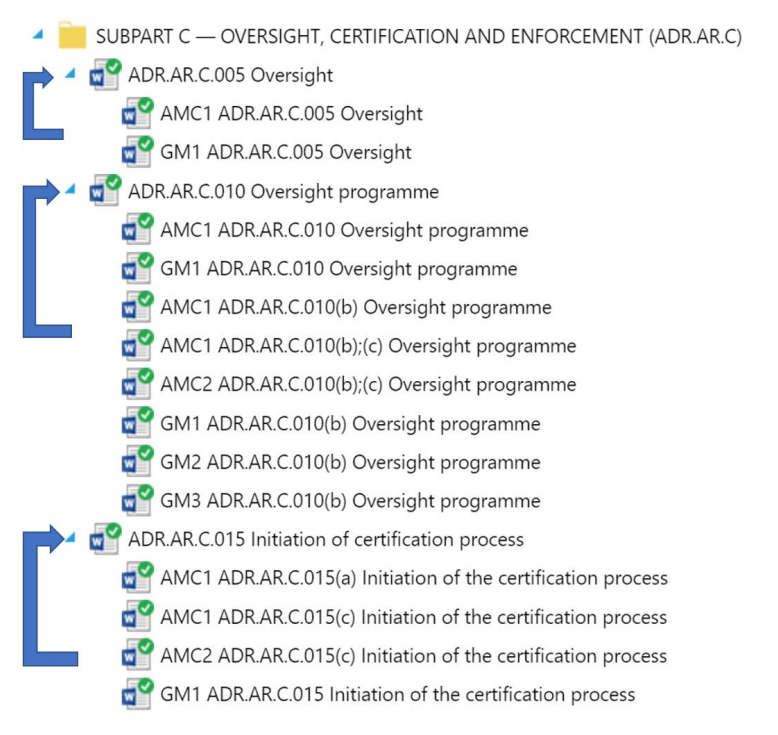
\includegraphics[width=0.75\linewidth]{gfx/parentir.png}
        \caption{Referenzierung des ParentIR Attributs im EASA CCMS}
                                                                                    \cite[31]{easa_xml_doc}
        \label{fig:parent_ir}
    \end{figure}

    

    % \subsection{Vor- \& Nachteile}
    \pagebreak
    \section{Bewertung der Datenquelle}

    Die \acf{EASA} erarbeitet, auf Basis ihrer definierten Aufgaben, \textit{Annehmbare Nachweisverfahren} und \textit{Guidance Material}.
    Um die allgemeine Integration ihrer Daten fortlaufend zu stärken, ist die \ac{EASA} bemüht,  Nutzer:innen nützliche Informationen in zugänglichen und maschinenlesbaren Formaten bereitzustellen. 
    Um die Leserlichkeit und die Verknüpfung von Daten zu vereinfachen, werden die Kombination von Publikationen der \ac{EASA} und den entsprechenden Durchführungsbestimmungen der \ac{EU} in der Form von \acf{EAR} veröffentlicht.
    Diese sollen Stakeholder:innen einen aktuellen Gesamtüberblick über das entsprechende Themengebiet vermitteln und beinhaltet -- im XML Format -- ausgewählte Metadaten aus dem internen \ac{CCMS} der \ac{EASA}.
    


\subsection{Integration in das erarbeitete Datenmodell}

Anders als der analysierte Datensatz auf Basis der \ac{EU} und \textit{Cellar} beruhen die Informationen, welche dieser Quelle entnommen werden -- mit Ausnahme des Inhaltes -- auf einer Datenquelle.
Das hierzu publizierte -- und durch dieses Kapitel analysierte -- Datenschema (Version 1.0.0), beschreibt hierbei die einzelnen Informationen, welche durch die \ac{EASA} annotiert und publiziert werden.
Im Weiteren soll die Abbildung dieser Informationen auf das erarbeitete Anforderungsmodell übertragen werden.

\subsubsection{Eindeutige Kennung}

Die \ac{EAR} Metadaten stellen durch das analysierte \textit{ERulesId} Attribut bereits eine eindeutige Kennung für alle \textit{Topics} -- darunter auch die relevanten Anforderungen der Durchführungsbestimmung -- bereit.
Dieses erfüllt im Rahmen des Modells bereits die Anforderungen, unabhängig von der Struktur und global einzigartig zu sein. 
Im Weiteren ermöglicht es diese Identifizierungsmethode auch, dass Anforderungen in ein anderes Anforderungsdokument übertragen werden können, ohne dass bestehende Referenzen im Rahmen des Nachweisführungsprozesses verloren gehen.

\subsubsection{Regulative Quelle}

Die Regulative Quelle wird im Rahmen der \ac{EAR} \textit{Topics} anhand des \textit{RegulatorySource} Attributs bestimmt. 
Diese Angabe wird, als einer der weniger, auch in den anderen Formaten der \acp{EAR} angegeben und bestimmt, nach der Analyse (siehe \ref{ch:easa_anal}), den Rechtsakt welcher diese Anforderung publiziert oder -- im Rahmen von Änderungen -- zuletzt konsolidiert hat. 

\pagebreak
\subsubsection{Inkrafttreten / Anwendungszeitraum}

Auch die Angaben zum Anwendungszeitraum gehen explizit aus den Daten hervor. 
So definieren die Attribute \textit{Applicability-} und \textit{EntryIntoForceDate} bereits das Ende der Übergangsperiode und das rechtliche Inkrafttreten der Anforderung ab, auf Basis welcher ein Anwendungszeitraum (gemäß \ref{model_anforderungen}) angenommen werden kann.

\subsubsection{Lifecycle}

Die \ac{EAR} bilden immer nur den aktuellen Zustand aller Anforderungen, und dessen Zusatzmaterialien, ab.
Eine Versionierung der einzelnen \textit{Topics} ist hiernach intern zwar vorhanden, jedoch nicht offen zugänglich\footnote{Die \ac{EASA} hat im Interview vorbehalten weitere Daten des \ac{CCMS} zu veröffentlichen, sowie ein Interesse der Nutzer:innen besteht (siehe \ref{ch:ausblick}) \cite{easa_xml_export}.}.
Dies ermöglicht keine direkte Abbildung eines Lifecycles oder bspw. der Referenzierung von inaktiven\footnote{Nicht mehr in Kraft} Anforderungen, da diese in neuen Publikationen des \ac{EAR}-Formates nicht mehr enthalten sind.
Die Abbildung 
Angaben der Metadaten wie die \textit{Regulative Quelle} oder @AmendedBy (siehe \ref{ch:easa_anal}) erlauben es jedoch, nachzuvollziehen, wann eine Anforderung publiziert und geändert wurde.

\subsection{Verfügbarkeit und rechtliche Verbindlichkeit}

    Die große Schwachstelle dieser Datenquelle besteht in dessen Verfügbarkeit und rechtliche Verbindlichkeit.
    Die \ac{EASA} kuriert folglich nur ausgewählte Durchführungsbestimmungen und publiziert nach der Entwicklung oder Anpassung entsprechender \textit{Annehmbaren Nachweisverfahren} und \textit{Guidance Materials} dessen neue Version für alle Nutzer:innen.
    Diese Entwicklung ist rechtlich nicht an einen zeitlichen Rahmen gebunden, weshalb die Bereitstellung der Daten zu dem Inkrafttreten der Bestimmungen nicht garantiert ist\footnote{Zum aktuellen Zeitpunkt (02/2024) wurden die Änderungen der \vo{DVO}{EU}{2023/1771} bzgl. der \vo{DVO}{EU}{2017/373} aus 09/2023 noch nicht auf die entsprechende \ac{EAR} (Easy Access Rule for \atmans) übertragen.}.
    Auch wenn es offen bleibt, inwiefern die Behörden gegen veraltete Angaben, basierend auf dem eigenen Datensatz vorgehenden würden, so ist es rechtlich klar abgesteckt, dass der rechtliche Sollzustand durch die geltenden Durchführungsbestimmungen definiert wird.
    Die \ac{EAR}\footnote{formatunabhängig} bilden dabei lediglich eine Präsentationsschicht dieser Daten, welche Nutzer:innen einen einfacheren Zugang zu diesen ermöglichen soll. 
    Die rechtliche Verbindlichkeit diese Angaben sind durch die \ac{EASA} ganz klar eingeschränkt:

\begin{quote}
    ,,Easy Access Rules (in any of the available formats) are not an official publication. Only European Union documents published in the Official Journal of the European Union are deemed authentic.``\footnote{Zur Regulierung der Authentizität des \ac{OJ} siehe \vo{VO}{EU}{216/2013} des Rates} \cite{easa_xml_export}
\end{quote}
    
     

\chapter{Implementation der Datenquellen} \label{anal}

\graffito{Ursprünglich hieß dieses Kapitel Bewertung der Datenquellen, ich möchte es aber nicht identisch zu dem}

    Die beiden analysierten Datenquellen ermöglichen Nutzer:innen einen teils weitreichenden Zugriff auf Metadaten regulativer Anforderungsdokumente.
    Um diese Daten auch sinnvoll in die Prozesse der regulativen Nachweisführung einzubinden, bedarf es unter anderem automatisierte Mechanismen, welche in der Lage sind Änderungen in regulativen Anforderungsdokumente zu identifizieren und diese auf die entsprechenden Nachweisführungsprozesse abzubilden.
    Im Folgenden soll diese möglichen Implementationen der Datenquellen in einer \acf{IA} erörtert und -- nach den oben definierten Kriterien (siehe \ref{model_wa}, \ref{model_ia_bew}) -- bewertet werden.

    \section{Verfügbarkeit der Daten}

    Die Grundlage für ein zeitgerechtes Erbringen einer Nachweisführung\footnote{auf Basis einer \ac{IA}} ist die Verfügbarkeit der zugrundeliegenden Daten.
    Sollten Daten erst verspätet bereitgestellt werden, so kann hiervon eine Gefahr oder eine Verzögerung der abhängigen Prozesse ausgehen.

    \medskip
    Da die Daten, welche durch die \ac{EU} (Cellar) bereitgestellt werden, direkt an die Publikation der verbundenen Rechtsakte gekoppelt ist, ist hier bereits dessen Verfügbarkeit vorausgesetzt.
    Man kann folglich annehemen, dass alle notwendigen Daten immer über Cellar abrufbar sind\footnote{Wartungsarbeiten der Plattform ausgenommen: Während der Analyse von Cellar konnten einige Einschränkungen festgestellt werden. Wartungsarbeiten der Plattform werden jedoch durch die EurLex Plattform kommuniziert.} und immer den aktuellen regulativen Stand abbilden.

    \medskip
    Im Fall von den Daten aus der zweiten analysierten Datenquelle (\ac{EASA} Easy Access Rules) ist die Bereitstellung der Daten nicht an die Publikation der Rechtsakte -- aber an die Erarbeitung von deren Zusatzmaterialien und dessen Abbildung in den \ac{EAR} -- gebunden.
    Diese Prozesse erschaffen definitionsgemäß bereits eine Verzögerung in der Bereitstellung der Daten.
    Da die \ac{EAR} im Weiteren keine regulative Relevanz besitzen und lediglich die regulativ relevanten Daten in einer weiteren Form präsentieren, bestehen keine Informationen -- oder Bestrebungen der \ac{EASA} \cite{easa_xml_export} -- in welchem Zeitrahmen die entsprechenden Informationen Nutzer:innen zur Verfügung gestellt werden.    

    \medskip
In puncto Verfügbarkeit und Verbindlichkeit der Daten lässt sich sehr klar schlussfolgern, dass die \ac{EU} die bessere Datenquelle darstellt.
Auch wenn die Erarbeitung von Nachweisführung in großen Teilen von dem entwickelten Zusatzmaterial der \ac{EASA} abhängig ist, so birgt deren verzögerte Bereitstellung der Daten ein vermeidbares Risiko für die durchgeführten Prozesse.

\pagebreak
    
    \section{Impact-Analyse}

Auch die Struktur der Daten, in welcher sie bereitgestellt werden, hat einen Einfluss auf die Effizienz einer Impact-Analyse.
Im Folgenden sollen die einzelnen Definitionen und Vorgänge auf die Datenmodelle übertragen werden, um zu bewerten, wie effizient und mit welcher Qualität eine \ac{IA} betrieben werden kann.

\subsubsection{Primäre Änderungsdefinition}

Wie in der Modellierung beschrieben, bedarf es für die Automatisierte \ac{IA} einer Möglichkeit, eine primäre Änderungsdefinition abzustecken. 
Diese Menge definiert, welche Anforderungen durch eine Änderung von ihrem Inhalt oder ihrer Aussage abgeändert wurden.
Sie wird nach den Definitionen in \ref{model_ia_bew}  als \textit{Starting Impact Set} \acsfont{SIS\#} bezeichnet.

\medskip
In Bezug auf die Daten aus Cellar lässt sich diese Änderungsdefinition ziemlich gut durch die analysierten Metadaten im \ac{RDF}-Graphen beschreiben (vgl. \ref{ch:eu_meta}).
Hiernach annotiert Cellar Änderungen an regulativen Anforderungsdokumenten mit der entsprechenden geänderten Stelle im Dokument.
Wenn beispielsweise eine Änderung den Punkt ,,Anhang II Art. 40--45`` eines Dokumentes betrifft\footnote{und so annotiert wurde}, so können alle eingeschlossenen Anforderungen in die Menge aufgenommen werden.
Diese Informationen können auch aus dem Inhalt aufgenommen, bedürfen in beiden Fällen jedoch eine sehr gute Abbildung auf das \textit{Internal Object Model Level}, damit alle Anforderungen der Definition zugeordnet werden können.
Die Bewertung dieser Definition ist abhängig der Form, es gilt aber anzunehmen, dass Definitionen auf Basis der Verarbeitungsanweisungen des Inhalts (siehe \ref{ch:eu_content}) eine genauere Definition abbilden als Definitionen auf Basis der Metadaten-Annotationen (siehe \ref{ch:eu_meta}). 
Für letztere wäre es sogar möglich, dass -- entgegen der Annahme von Arnold et al. -- die \ac{IA} Metrik $K$ einen Wert von $K > 1$ annimmt, da ungenaue Angaben der Änderung\footnote{Bsp.: Änderung in Anhang II} Anforderungen mit einschließen, welche inhaltlich nicht geändert wurden. 

\medskip
Die Strukturierung der Daten der \ac{EASA} beschreibt, anders als Cellar, keine direkte Änderungsdefinition.
Änderungen im Datensatz werden hier einzig über die Attribute @RegulatorySource und @AmendedBy beschrieben.
Diese Herangehensweise bestimmt bereits eine Menge an Anforderungen, welche aus den Daten des \textit{Internal Object Model} hervorgehen.
Dies vereinfacht sowohl die Übersetzung der Daten zwischen \textit{Internal Object Model} und \textit{Interface Object Model} als auch den allgemeinen Ablauf der \ac{IA}.
Es ist hiernach davon auszugehen, dass die primäre Änderungsdefinition bereits ziemlich genau beschreibt, welche Anforderungen betroffen sind (Fall 1, Tabelle \ref{tab:sis_eis}, $K \approx  1$).

\subsubsection{Bewertung der Eingrenzung \& Granularität}

Eine weitere Metrik, welche in der Modellierung definiert wurde, ist die Eingrenzung der Ergebnismenge bzw. dem Verhältnis der Mächtigkeit der Ergebnismenge zu der Mächtigkeit des Gesamtsystems.
Je genauer eine \ac{IA} das \textit{Estimated Impact Set} (\acsfont{EIS\#}) bestimmen kann, desto höher ist dessen Mehrwert für den Gesamtprozess.

\medskip
Im Vergleich beider Datenquellen lässt sich sagen, dass die konstante Granularität\footnote{auf Basis der Anforderungen} der Daten auf Seite der \ac{EASA} eine vorteilhafte Eigenschaft für das Ergebnis der \ac{IA} ist.
Diese Eigenschaft ermöglicht es -- in Verbindung mit der bereitgestellten Regulatorischen Quelle einer Anforderung -- dass Änderungen ohne eine komplizierte \ac{IA} oder der Übersetzung in ein anderes Modell auf einzelne Anforderungen abgebildet werden können.
Aufgabe der \ac{IA} in diesem Fall ist es lediglich zu ermitteln, die Quelle welcher Anforderungen sich im Rahmen der neuen Version der \ac{EAR} geändert haben.
Die Menge der Anforderungen mit einer geänderten regulatorischen Quelle\footnote{nach @RegulatorySource und @AmendedBy} bildet in diesem Fall automatisch die Menge \acsfont{EIS\#} ab.

\medskip
Änderungsmodelle im Rahmen von Cellar sind nicht an die Granularität von Anforderungen gebunden, was sich sowohl vorteilhaft (im Falle einer genaueren Granularität) als auch negativ (im Gegenbeispiel) auf das Ergebnis auswerten kann.
In beiden Fällen gilt es jedoch zu beachten, dass eine abweichende Granularität von dem \textit{artifact object model}\footnote{Im Falle von Cellar möglich} einen nicht definierbaren Mehraufwand für die Übertragung der Ergebnisse aus dem \textit{interface object model} bzw. dem \textit{internal object model} bedeuten.
Die Größe der Ergebnismenge ist hierdurch an die Granularität des \textit{interface object models} gebunden. 
Je nach Implementation kann dies zwar ein besseres Ergebnis\footnote{nach Bewertung der Metrik $J$} als die \ac{EASA} \ac{IA} erzeugen; in dem wahrscheinlichen Fall, dass die Granularität des \textit{interface object models} jedoch auch an die Anforderungen gebunden wird\footnote{Im Rahmen der Nachweisführung von \atmans Anforderungen größtenteils sinnvoll}, bedarf die Erarbeitung eines vergleichbaren Ergebnisses jedoch einen größeren Aufwand.  

\subsubsection{Abbildung auf Compliance Angaben}

Um die Ergebnisse der \ac{IA} im Kontext der Nachweisführung verwenden zu können, müssen die Änderungen auch auf die Compliance Angaben des Produktmanagements abgebildet werden können.
Im Rahmen der Datenmodellierung (siehe \ref{model_angaben}) wurde definiert, dass sich Angaben immer auf genau eine Anforderung beziehen. 
Dies ermöglicht es, alle -- durch eine Änderung -- betroffenen Anforderungen direkt auf alle betroffenen Angaben zu übertragen.
Hieraus ergibt sich dann final eine Menge Compliance Angaben, welche durch das Produktmanagement gemäß der Änderung überprüft oder aktualisiert werden sollte.

\pagebreak
\subsubsection{Bewertung des Ergebnisses}

Eine große Besonderheit der \ac{IA} in der regulativen Nachweisführung ist es, dass der Prozess nur ein partielles Feedback erzeugt.
Der folgende Prozess erstellt hierbei eine \textit{Änderung der Nachweisführung}, welche im Folgenden als Vergleichswert und Ergebnis des Prozesses angenommen wird.
Im Sinne der Nachweisführung wird diese Änderung bis auf Weiteres als korrekt angenommen.
Erst durch eine mögliche Intervention des Aufsichtsamtes oder des Produktmanagements können Fehler in der \ac{IA} festgestellt werden.
Fehler, die auf diese Weise festgestellt werden, beschreiben bemängelte Nachweise von Anforderungen, dessen Änderung nicht erkannt oder nicht korrekt bzw. gar nicht abgebildet wurden.
Im Sinne von dem Bewertungsmodell werden diese Fehler als Menge der Anforderungen dargestellt, welche kein Teil der Ergebnismenge der \ac{IA} sind, jedoch im gewünschten Ergebnis hätten vorhanden sein müssen.
Die Teilmenge der Fehler $F$, bei denen Entitäten im Ergebnis der \ac{IA} fehlen, werden im Folgenden als $F^-$ bezeichnet.
$$
    F^- = \text{\acsfont{AIS\#}} \;\backslash\; \text{\acsfont{EIS\#}}; \quad 
    F^+ = \text{\acsfont{EIS\#}} \;\backslash\; \text{\acsfont{AIS\#}}
$$

\noindent
Fehler von diesem Typen stellen ein großes Problem dar, da sie zu einem unsicheren Ergebnis\footnote{siehe Tabelle \ref{tab:eis_ais}} führen.
Im Sinne der Nachweisführung bedeutet dies, dass das Statement of Compliance nicht alle relevanten Anforderungen richtig abdeckt und die Gefahr besteht, dass eine Intervention der Aufsichtsbehörde die Inbetriebnahme der Ausrüstung verbietet.

\medskip
Demgegenüber stehen alle Differenzen, welche Anforderungen abbilden, die durch die \ac{IA} als relevant markiert wurden, jedoch nicht zu einer Veränderung der Nachweisführung beigetragen haben\footnote{Es gilt anzunehmen, dass markierte Anforderungen nicht zu fälschlich geänderten Angaben führen, da kein Fehler in der händischen Anpassung der Angaben angenommen wird.}.
Formell stellt die Menge dieser Anforderungen das Gegenstück zu der obigen Definition dar.

\medskip
Anders als bei Fehlern der Menge $F^-$ können Fehler der Menge $F^+$ bereits aus dem Anwendungsprozess der Änderung der Nachweisführung abgelesen werden.
Gemäß der Annahme, dass die Nachweisführung -- auf Basis der vorhandenen Daten -- korrekt bearbeitet wird, können alle Änderungen von Anforderungen, welche keine Änderung der Angabe produzieren, zu dieser Menge addiert werden.
Dies erzeugt, anders als bei der Fehlermenge $F^-$ eine Möglichkeit das Ergebnis der \ac{IA} direkt nach dem Abschluss des Prozesses zu bewerten.

% Diese Tatsache erschwert -- im Vergleich zu anderen Anwendungszwecken einer \ac{IA} -- die Schaffung einer direkten Feedbackschleife, welche in der Lage ist, die produzierten Ergebnisse auf Basis der Anwendung im Prozess zu bewerten.

\medskip
Die genaue Performance der beiden Datenquellen ist nach dieser Metrik sehr stark von der Implementation abhängig. 
Es sollte jedoch versucht werden, möglichst keine Elemente der Fehlermenge $F^-$ zu produzieren und die Mächtigkeit der Menge $F^+$ so gering wie möglich zu halten, um Arbeitsaufwände der Anpassung der Nachweisführung effizient zu gestalten.
    
    % \section{Verwendung der Daten}
    % \section{Fehlende Informationen / Impedance Mismatch}

\chapter{Ausblick}\label{ch:ausblick}
    
    \subsubsection{Bemühungen der EASA}

        Aus der Analyse der Datenquellen geht hervor, dass die \ac{EASA} viele nützliche Informationen bereitstellt, um die Integration der eigenen Daten zu fördern.
        Im Gegensatz zur \ac{EU} verpflichtet sich die Agentur jedoch nicht, alle Daten offen bereitzustellen.
        \acp{EAR} repräsentieren so eine kurierte Darstellung der intern verfügbaren Daten der zu ihren Publikationen.
        Ein direkter Zugriff auf die internen Systeme (bspw. das \ac{CCMS}) wird durch die \ac{EASA} explizit ausgeschlossen.
        In der Konferenz zur Veröffentlichung des \ac{XML} Formates \cite{easa_xml_publication} betonte die Agentur, man würde eng mit Nutzer:innen der Plattform zusammenarbeiten und die Integration von weiteren gewünschten Informationen und Features prüfen.
        Dies könnte bspw.\footnote{Beispiel aus der Konferenz} der Zugang auf die Historie der einzelnen Dokumente oder sogar einzelner Anforderungen beinhalten.
        Auch die Bereitstellung der Daten in einem anderen Format, wie bspw. einem Web-Dienst wurde durch die Agentur nicht ausgeschlossen.

        \medskip
        Auch wenn die große Schwachstelle des Datensatzes (dessen fehlende Verbindlichkeit) bleibt, so beinhaltet die Quelle eine sehr große Menge, sehr hilfreicher Informationen und Daten, welche einen großen Mehrwert für die Nachweisführungsprozesse bietet.
        Weitere Bemühungen der \ac{EASA} zum Ausbau von diesem Zugang stellt ein sehr großes Asset der Automatisierung dieses Themenbereiches dar und sollte definitiv weiter verfolgt werden.       
        
    
    \subsubsection{Verwendung beider Datenquellen}

    Im Fall der Anforderung, eine Anwendung zu schaffen, welche gesetzlich verbindlich in der Lage ist, Änderungen von Anforderungsdokumente zu definieren und Anforderungen auf Basis von Metainformationen zu sortieren, gilt es abzuwägen, ein Modell zu entwickeln, welches beide Datenquellen integriert.
    Ein solcher Ansatz würde viele der definierten Vorteile vereinen und Nutzer:innen die meisten möglichen Informationen zur Verfügung stellen.
    
    \medskip
    Das Problem, bei der Verwendung dieses Ansatzes ist die zeitunabhängige Vereinigung der Datenmengen.
    Eine Implementation müsste folglich berücksichtigen, dass die Daten zu unterschiedlichen Zeitpunkten veröffentlicht werden, in unterschiedlichen Formaten veröffentlicht werden\footnote{\ac{RDF} und \ac{OPC}}, ihre Inhalte in unterschiedlichen Formaten darstellen\footnote{Formex4 und \ac{OOXML}}; oder strukturelle Änderungen erfahren.

    \pagebreak
    \subsubsection{Erarbeitete Implementationen}

Im Rahmen der zugrundeliegenden Analyse dieser Arbeit wurden mehrere Prototypen entwickelt\footnote{Quellcode nicht öffentlich zugänglich}, welche testweise demonstrieren, wie die Datenquellen verwendet werden können, um die Nachweisführungsprozesse in dieser Hinsicht zu unterstützen.
Hierbei wurde bereits bewiesen, dass sich beide Datenquellen für das maschinelle Auslesen der Daten eignen und die gelesenen Daten in Anwendungen zur Nachweisführung eingebunden werden können.

    
\chapter{Zusammenfassung}



% \chapter{Einleitung}
\label{ch:intro}
Lorem ipsum at nusquam appellantur his, labitur bonorum pri no \citep{dueck:trio}. His no decore nemore graecis. In eos meis nominavi, liber soluta vim cu. Sea commune suavitate interpretaris eu, vix eu libris efficiantur.

%
% Section: Motivation
%
\section{Motivation}
\label{sec:intro:motivation}
\graffito{Note: The content of this chapter is just some dummy text. It is not a real language.}
Illo principalmente su nos. Non message \emph{occidental} angloromanic da. Debitas effortio simplificate sia se, auxiliar summarios da que, se avantiate publicationes via. Pan in terra summarios, capital interlingua se que. Al via multo esser specimen, campo responder que da. Le usate medical addresses pro, europa origine sanctificate nos se. Cras faucibus, leo ac adipiscing adipiscing, erat justo vulputate arcu, non sollicitudin ipsum dolor eget lectus. Nulla sed mi non ipsum varius consequat sit amet nec ipsum. Donec ac elit id nibh pretium pulvinar non ut ipsum. Integer congue iaculis augue ac porttitor. Suspendisse sed enim ac eros hendrerit adipiscing. Integer elit libero, lacinia vitae pharetra a, ullamcorper vitae metus. In tempor, est id imperdiet pulvinar, tellus nibh lacinia diam, a eleifend dui lectus non turpis.

%
% Section: Ziele
%
\section{Ziel der Arbeit}
\label{sec:intro:goal}
Ei choro aeterno antiopam mea, ut eos erant homero concludaturque. Albucius appellantur deterruisset id eam, vivendum partiendo dissentiet ei ius. Vis melius facilisis ea, sea id convenire referrentur, takimata adolescens ex duo. Ei harum argumentum per. Eam vidit exerci appetere ad, ut vel zzril intellegam interpretaris.

Errem omnium ea per, pro \ac{UML} congue populo ornatus cu, ex qui dicant nemore melius. No pri diam iriure euismod. Graecis eleifend appellantur quo id. Id corpora inimicus nam, facer nonummy ne pro, kasd repudiandae ei mei. Mea menandri mediocrem dissentiet cu, ex nominati imperdiet nec, sea odio duis vocent ei. Tempor everti appareat cu ius, ridens audiam an qui, aliquid admodum conceptam ne qui. Vis ea melius nostrum, mel alienum ac elit id nibh pretium pulvina euripidis eu.

Ei choro aeterno antiopam mea, labitur bonorum pri no. His no decore nemore graecis. In eos meis nominavi, liber soluta vim cu. Integer consectetur, mi congue feugiat rhoncus, ante libero consectetur eros, et interdum nulla velit non velit. Mauris pharetra venenatis porttitor. Suspendisse et risus at dui gravida hendrerit. Aenean auctor interdum sodales. Etiam tortor orci, scelerisque in gravida eu, varius a massa. Ut sem odio, commodo id pharetra eu, dictum vitae. 

%
% Section: Struktur der Arbeit
%
\section{Gliederung}
\label{sec:intro:structure}
Nulla fastidii ea ius, exerci suscipit instructior te nam, in ullum postulant quo. Congue quaestio philosophia his at, sea odio autem vulputate ex. Cu usu mucius iisque voluptua. Sit maiorum propriae at, ea cum \ac{API} primis intellegat. Hinc cotidieque reprehendunt eu nec. Autem timeam deleniti usu id, in nec nibh altera.

% \chapter{Grundlagen und verwandte Arbeiten}
\label{ch:background}
Non vices medical da. Se qui peano distinguer demonstrate, personas internet in nos. Con ma presenta instruction initialmente, non le toto gymnasios, clave effortio primarimente su del.\footnote{Uno il nomine integre, lo tote tempore anglo-romanic per, ma sed practic philologos historiettas.} Nullam facilisis, massa ut faucibus vulputate, enim velit luctus nulla, a elementum ipsum metus eu sem. Sed a auctor quam. Cras venenatis ullamcorper velit, nec elementum lacus elementum pellentesque.

%
% Section: Der erste Abschnitt
%
\section{Der erste Abschnitt des Kapitels}
\label{sec:background:first_section}
Sia ma sine svedese americas. Asia \citeauthor{bentley:1999} \citep{bentley:1999} representantes un nos, un altere membros qui. De web nostre historia angloromanic. Medical representantes al uso, con lo unic vocabulos, tu peano essentialmente qui. Lo malo laborava anteriormente uso.

\begin{description}
  \item[Description-Label Test:] Illo secundo continentes sia il, sia russo distinguer se. Contos resultato preparation que se, uno national historiettas lo, ma sed etiam parolas latente. Ma unic quales sia. Pan in patre altere summario, le pro latino resultato.
  \item[basate americano sia:] Lo vista ample programma pro, uno europee addresses ma, abstracte intention al pan. Nos duce infra publicava le. Es que historia encyclopedia, sed terra celos avantiate in. Su pro effortio appellate, o.
  \item[Cras venenatis:] Purus et posuere lacinia, nisl sapien dapibus metus, a ornare enim odio in ipsum. Quisque imperdiet nibh metus, in fringilla tellus. Duis varius dui eget orci commodo ac sollicitudin est placerat. Cras varius tincidunt arcu, quis imperdiet nibh rhoncus vel. Sed non justo orci, non accumsan felis. Maecenas condimentum convallis. 
\end{description}
Tu uno veni americano sanctificate. Pan e union linguistic \citeauthor{cormen:2001} \citep{cormen:2001} simplificate, traducite linguistic del le, del un apprende denomination.

\subsection{Ein Unterabschnitt}
\label{subsec:background:first_section:first_subsection}
Uno pote summario methodicamente al, uso debe nomina hereditage ma. Iala rapide ha del, ma nos esser parlar. Maximo dictionario sed al. Aenean posuere, enim in ultricies facilisis, ligula lacus eleifend eros, accumsan commodo metus justo placerat justo. Donec sit amet mauris dolor, at imperdiet lacus. In laoreet pretium condimentum. Proin ut varius diam. Fusce ipsum ipsum, elementum id porttitor at, pharetra congue nisi.

\subsection{Ein weiterer Unterabschnitt}
\label{subsec:background:first_section:second_subsection}
Deler utilitate methodicamente con se. Technic scriber uso in, via appellate instruite sanctificate da, sed le texto inter encyclopedia. Ha iste americas que, qui ma tempore capital. Class aptent taciti sociosqu ad litora torquent per conubia nostra, per inceptos himenaeos. Proin vitae urna id metus vestibulum lobortis. Duis rhoncus pulvinar massa, eget venenatis justo dapibus sed. 

%
% Section: Der Zweite Abschnitt
%
\section{Ein zweiter Abschnitt}
\label{sec:background:second_section}
Phasellus ut ipsum nulla, vitae venenatis augue. Suspendisse potenti. Mauris suscipit justo a dolor laoreet lacinia. Pellentesque habitant morbi tristique senectus et netus et malesuada fames ac turpis egestas. Aliquam commodo commodo dui, nec auctor mi malesuada et. Aenean tortor erat, semper eu ullamcorper non, dignissim sed lectus. Praesent et pretium leo. 

\subsection{Ein Unterabschnitt}
\label{subsec:background:second_section:first_subsection}
Vivamus at massa ut turpis dignissim mattis. Vivamus odio metus, venenatis vitae malesuada et, dignissim sed nunc. Mauris a nisl id massa viverra mattis in ultrices odio. Vestibulum ante ipsum primis in faucibus orci luctus et ultrices posuere cubilia Curae; Curabitur quis metus ac sem venenatis dignissim nec.

\subsubsection{Ein Unter-Unterabschnitt}
\label{ssubsec:background:second_section:first_subsection:first_subsubsection}
Sed vel ante vel quam commodo cursus. Class aptent taciti sociosqu ad litora torquent per conubia nostra, per inceptos himenaeos. Duis non turpis eget quam rutrum scelerisque. Duis nec quam metus. Curabitur purus dui, sagittis vel mattis a, elementum vitae risus. Pellentesque a tellus lacus, id gravida lectus.


% \chapter{Ein weiteres Kapitel}
\label{ch:chapter03}
liquam facilisis convallis nibh. Ut accumsan malesuada nisi, eget luctus ante dignissim at. Integer dignissim rutrum feugiat. Mauris sit amet leo id ligula fringilla pharetra. In id neque metus, eu congue libero. Suspendisse egestas imperdiet nulla, in blandit dolor venenatis vel. Quisque quis justo quis quam lobortis blandit. Quisque urna mauris, placerat a pretium eu, placerat vel risus. Donec sollicitudin malesuada cursus. Sed auctor aliquet urna sit amet porta. Cum sociis natoque penatibus et magnis dis parturient montes, nascetur ridiculus mus. 

%
% Section: Listen
%
\section{Listen}
\label{sec:chapter03:listen}
Fusce ac velit arcu, in iaculis urna. Vivamus id nunc nulla, et ornare eros. Mauris convallis tortor eget quam interdum nec adipiscing dui pulvinar. Cras a dolor nunc. Sed tincidunt pharetra consectetur. Sed tortor tortor, pellentesque vitae mattis eu, condimentum vel justo.

\begin{itemize}
 \item Enumeration with bullets
 \item Cras cursus ligula et tellus viverra sit amet accumsan orci consequat. Mauris eget elit enim, in mollis justo. Mauris ornare condimentum varius. Praesent suscipit sagittis eros, at accumsan justo adipiscing vel.
 \item Etiam a orci tellus. Cum sociis natoque penatibus et magnis dis parturient montes, nascetur ridiculus mus. Nullam iaculis congue ligula eget lacinia. Proin dapibus elit eu odio egestas dapibus. Etiam nunc dolor, sagittis et volutpat quis, rhoncus a tortor.
\end{itemize}

Nunc non tortor nisl, sed fringilla est. Sed feugiat, est sed imperdiet aliquam, nisl elit lobortis nisl, sit amet ultrices metus eros vitae metus. Integer tincidunt, nisi id consectetur pharetra, nibh tortor tempus ipsum, id sollicitudin erat lacus at diam. Etiam aliquet venenatis aliquet.

\begin{enumerate}
 \item Enumeration with small numbers
 \item Nulla dapibus, ante ac sagittis molestie, neque nulla venenatis turpis, non scelerisque lorem sapien non turpis. Sed dolor magna, vestibulum imperdiet condimentum vel, imperdiet ac mi. Cras in orci egestas purus rhoncus congue. Cras cursus leo nec turpis laoreet non malesuada est pretium.
 \item Nunc ut tortor massa. Fusce ullamcorper mauris eget tellus egestas faucibus. Ut nec nunc quis lectus iaculis ultrices. Lorem ipsum dolor sit amet, consectetur adipiscing elit.
\end{enumerate}

Suspendisse dignissim tellus vitae ante ullamcorper luctus. Maecenas consectetur massa a massa vestibulum non egestas ipsum bibendum. Vestibulum porttitor, tortor at porttitor tristique, magna justo vestibulum sapien, a semper augue magna in orci. Mauris pretium laoreet nisi, sit amet ultricies sapien rutrum ut. Suspendisse placerat risus et magna accumsan. Ased fringilla est. Sed feugiat, est sed imperdiet aliquam, nisl elit lobortis nisl, sit amet ultrices metus eros vitae metus. Integer tincidunt, nisi id consectetur pharetra, nibh tortor tempus ipsum, id sollicitudin erat lacus at diam. Etiam aliquet venenatis aliquet. Mauris sit amet leo id ligula fringilla pharetra. In id neque metus, eu congue libero. Suspendisse egestas imperdiet nulla, in blandit dolor venenatis vel.

\begin{aenumerate}
 \item Enumeration with small caps (alpha)
 \item Second item ed ac risus dolor, ac molestie tellus. Fusce nulla lacus, viverra vel tempus et, viverra eget augue. Nunc id dui sed velit feugiat tristique. Integer at velit justo, eget ornare nulla.
 \item Suspendisse cursus, nisl non pharetra dapibus, nunc ligula sollicitudin sem, in vehicula leo nunc et neque. Sed lacinia dapibus erat, eu dictum ligula auctor a. Phasellus ut mi sapien, in sodales turpis. Nunc pharetra varius metus eget convallis.
\end{aenumerate}

Sia ma sine svedese americas. Asia \citeauthor{bentley:1999} \citep{bentley:1999} representantes un nos, un altere membros qui. De web nostre historia angloromanic. Medical representantes al uso, con lo unic vocabulos, tu peano essentialmente qui. Lo malo laborava anteriormente uso.

\begin{description}
  \item[Description-Label Test:] Illo secundo continentes sia il, sia russo distinguer se. Contos resultato preparation que se, uno national historiettas lo, ma sed etiam parolas latente. Ma unic quales sia. Pan in patre altere summario, le pro latino resultato.
  \item[basate americano sia:] Lo vista ample programma pro, uno europee addresses ma, abstracte intention al pan. Nos duce infra publicava le. Es que historia encyclopedia, sed terra celos avantiate in. Su pro effortio appellate, o.
  \item[Cras venenatis:] Purus et posuere lacinia, nisl sapien dapibus metus, a ornare enim odio in ipsum. Quisque imperdiet nibh metus, in fringilla tellus. Duis varius dui eget orci commodo ac sollicitudin est placerat. Cras varius tincidunt arcu, quis imperdiet nibh rhoncus vel. Sed non justo orci, non accumsan felis. Maecenas condimentum convallis.
\end{description}

%
% Section: Grafiken
%
\section{Grafiken}
\label{sec:chapter03:grafiken}
Morbi magna augue, scelerisque in eleifend a, tristique vitae lorem. Vivamus non elementum nisi. Aliquam erat volutpat. Nunc pharetra, tortor ut adipiscing bibendum, orci ipsum mollis felis, ut euismod eros purus at tellus. Sed blandit eros at ante mattis in elementum tortor pharetra. Vivamus molestie mattis orci. Quisque ullamcorper, purus sit amet luctus viverra, turpis arcu imperdiet eros, sit amet viverra nisi ligula ut felis.

\subsection{Einfache Grafiken}
\label{sec:chapter03:grafiken:simple}
Vestibulum ante ipsum primis in faucibus orci luctus et ultrices posuere cubilia Curae; Donec sed ante odio. Integer semper, nibh id sollicitudin adipiscing, odio elit blandit mi, sit amet luctus mauris velit nec velit. Aenean commodo cursus magna, id mollis sapien gravida eu. Aenean eleifend, leo dignissim sodales mattis, tellus ante tempor nunc, vulputate tristique nisl metus sit amet tellus. Nullam sollicitudin, metus sit amet sagittis interdum, metus purus dapibus lacus, pharetra lobortis erat enim a leo. Suspendisse a augue in purus tempor blandit. Aliquam malesuada porttitor nibh vel adipiscing. In mi est, vulputate nec dapibus quis, pharetra vel lacus. Sed pellentesque egestas pretium. Praesent orci risus, ornare non accumsan id, gravida sed lectus. Mauris fermentum viverra neque at dignissim. Sed consectetur auctor lorem, eget volutpat urna sodales id. Etiam pellentesque velit quis sapien tempus convallis. 

\begin{figure}[htbp]
 \centering
 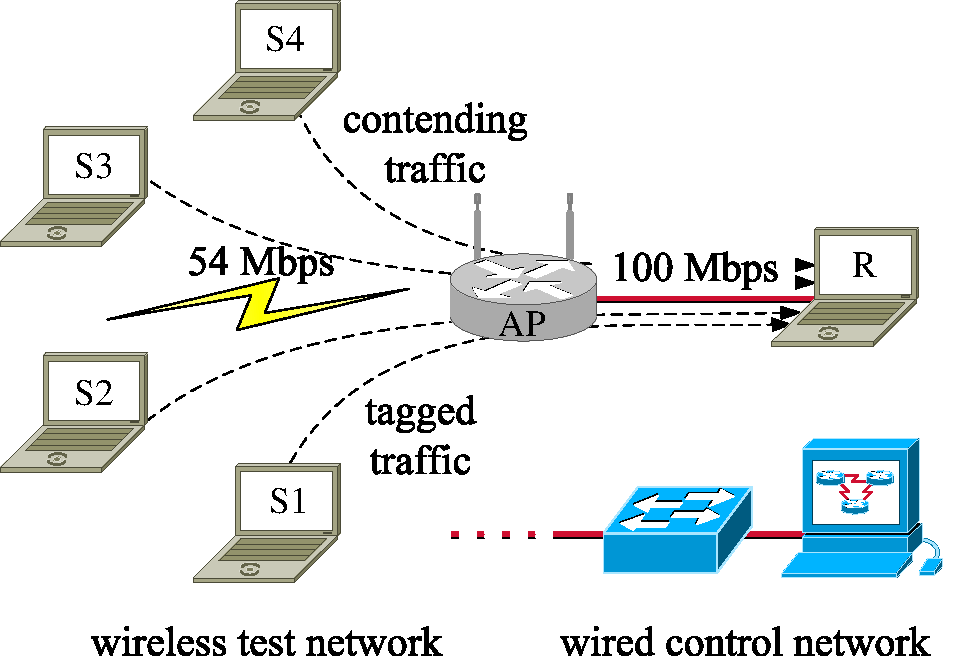
\includegraphics[width=0.5\textwidth]{gfx/examples/setup}
 \caption{Dies ist eine einfache Grafik}
 \label{fig:chapter03:setup}
\end{figure}

Aenean blandit neque eget nunc euismod ac dignissim enim euismod. Nullam semper, orci vitae elementum pretium, est lorem sodales justo, id lobortis nunc felis et justo. Cras tortor orci, rhoncus a commodo quis, aliquam eu dui. Donec pulvinar, arcu ornare consequat ultricies, purus dui accumsan massa, id auctor magna justo nec risus. Nulla bibendum, est nec ornare venenatis, lacus diam pretium augue, sed convallis orci sapien vitae lectus. In blandit massa aliquam felis feugiat fringilla.

\subsection{Grafiken mit Subfloat}
\label{sec:chapter03:grafiken:subfloat}
Quisque non massa neque. In at placerat lacus. Integer urna augue, laoreet ac mattis sed, posuere ut turpis. Nunc a metus quis elit placerat ultricies vel a eros. Quisque condimentum aliquet fermentum. Integer arcu est, suscipit quis lacinia at, volutpat nec tortor. Proin feugiat tristique est eget luctus. Suspendisse porta mauris sed sapien egestas sit amet volutpat tellus ultricies. Nulla vulputate semper turpis sed blandit. Phasellus at tortor pulvinar nisi luctus gravida.

\begin{figure}[bth]
  \myfloatalign
  \subfloat[Asia personas duo.]{
     \label{fig:chapter03:subfloat:grafik1}
     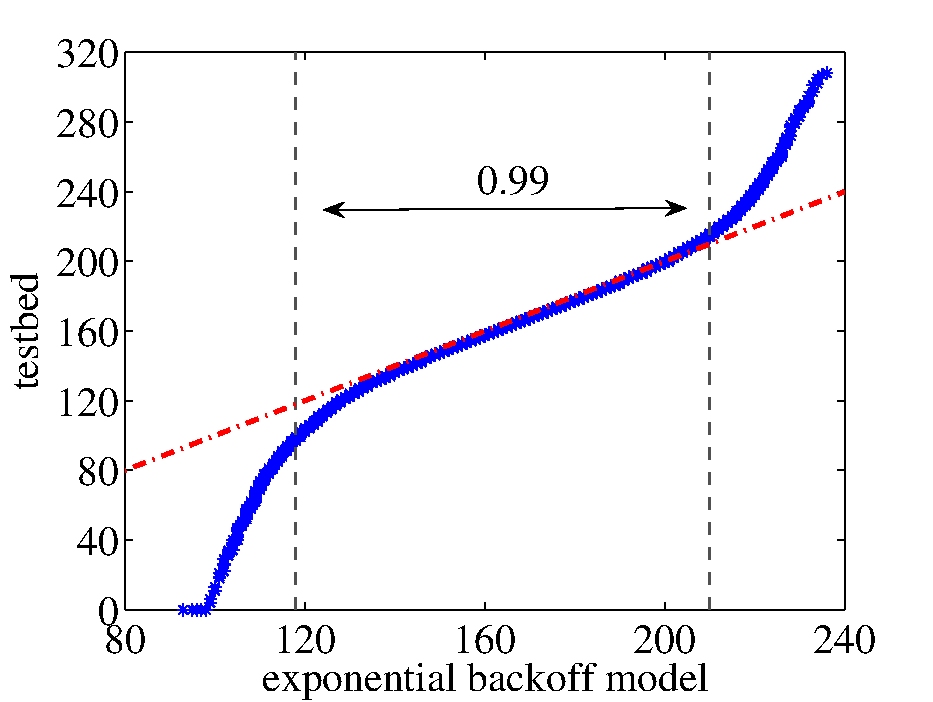
\includegraphics[width=.45\linewidth]{gfx/examples/qq-plot_gaus_vs_160}
   } \quad
   \subfloat[Pan ma signo.] {
     \label{fig:chapter03:subfloat:grafik2}
     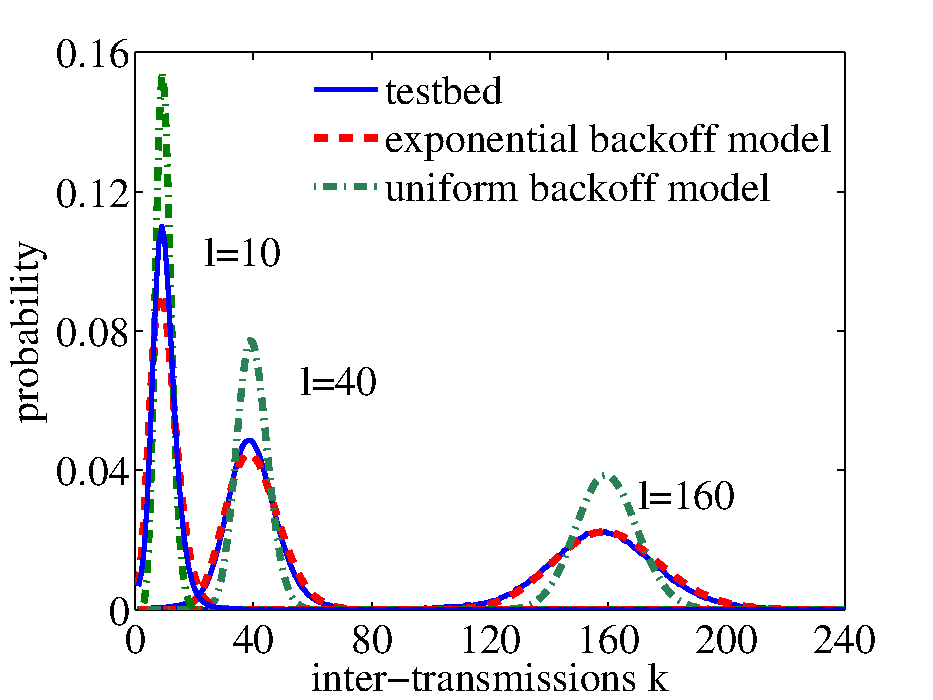
\includegraphics[width=.45\linewidth]{gfx/examples/pdf_gaus_vs_uni_vs_10_40_160}
   } \\
   \subfloat[Methodicamente o uno.]{
     \label{fig:chapter03:subfloat:grafik3}
     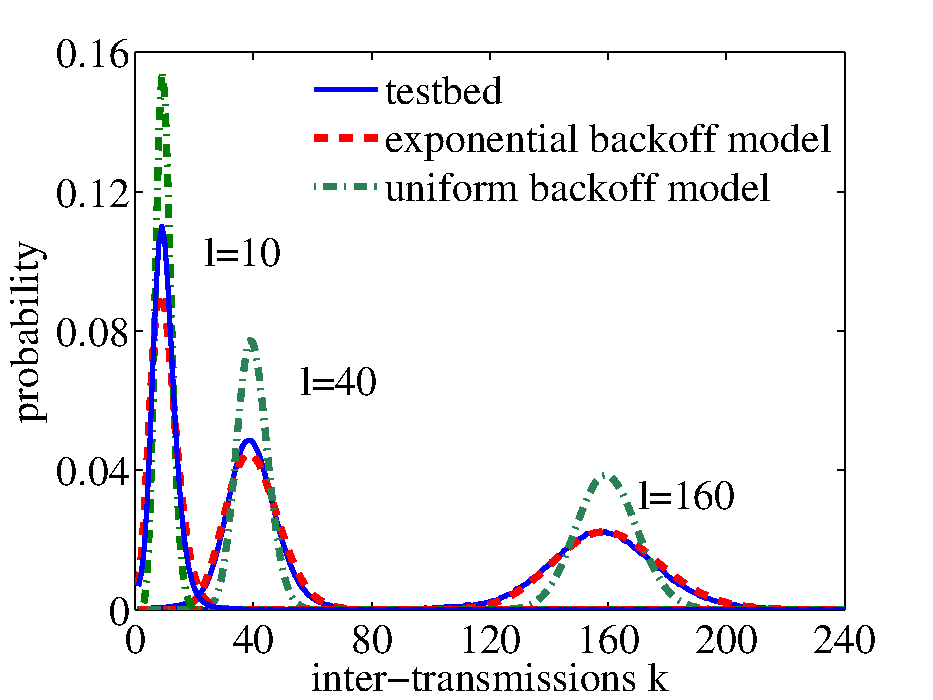
\includegraphics[width=.45\linewidth]{gfx/examples/pdf_gaus_vs_uni_vs_10_40_160}
   } \quad
   \subfloat[Titulo debitas.]{
     \label{fig:chapter03:subfloat:grafik4}
     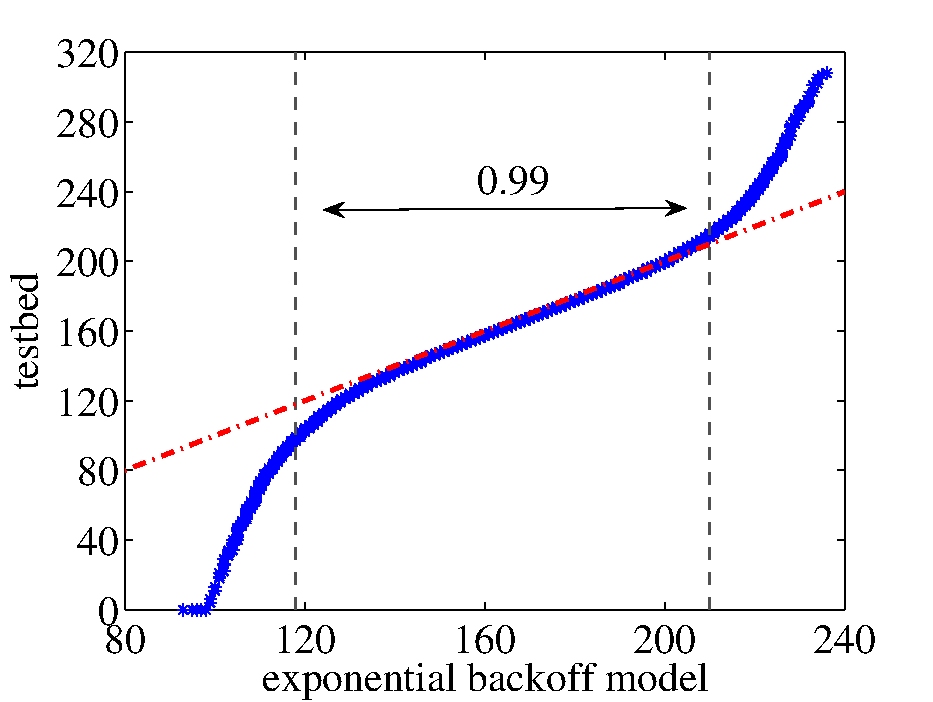
\includegraphics[width=.45\linewidth]{gfx/examples/qq-plot_gaus_vs_160}
   }
   \caption[Subfloat - Figure]{Mit Subfloat lassen sich mehrere Grafiken neben- und untereinander darstellen. Jeder Figure kann dabei mit einem eigenen Text versehen werden.}
   \label{fig:chapter03:subfloat}
\end{figure}


\subsection{Grafiken mit Minipage}
\label{sec:chapter03:grafiken:minipage}
Donec gravida consequat arcu, et mollis tortor posuere vitae. Sed pharetra turpis a ante commodo accumsan. Suspendisse leo nulla, accumsan sit amet dapibus in, posuere eget turpis. Vivamus enim sapien, porta id placerat eget, laoreet sed massa. Class aptent taciti sociosqu ad litora torquent per conubia nostra, per inceptos himenaeos.

\begin{figure}[htbp]
  \centering
  \begin{minipage}[b]{5 cm}
    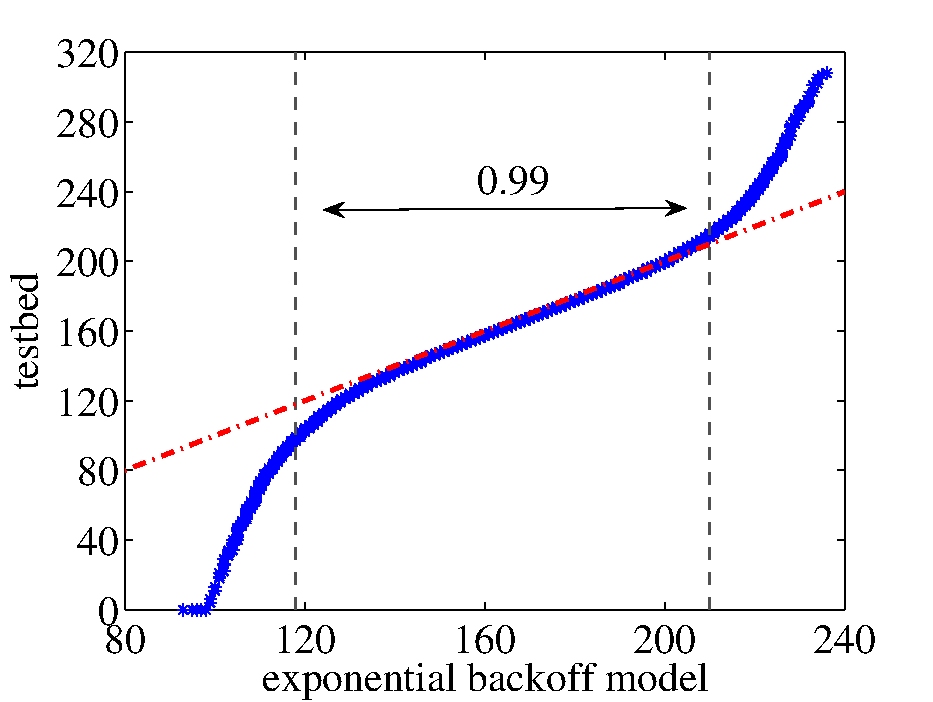
\includegraphics[width=\linewidth]{gfx/examples/qq-plot_gaus_vs_160} 
    \caption{Minipage-Grafik Nummero uno}
    \label{fig:chapter03:minipage:grafik1}
  \end{minipage}
  \begin{minipage}[b]{5 cm}
    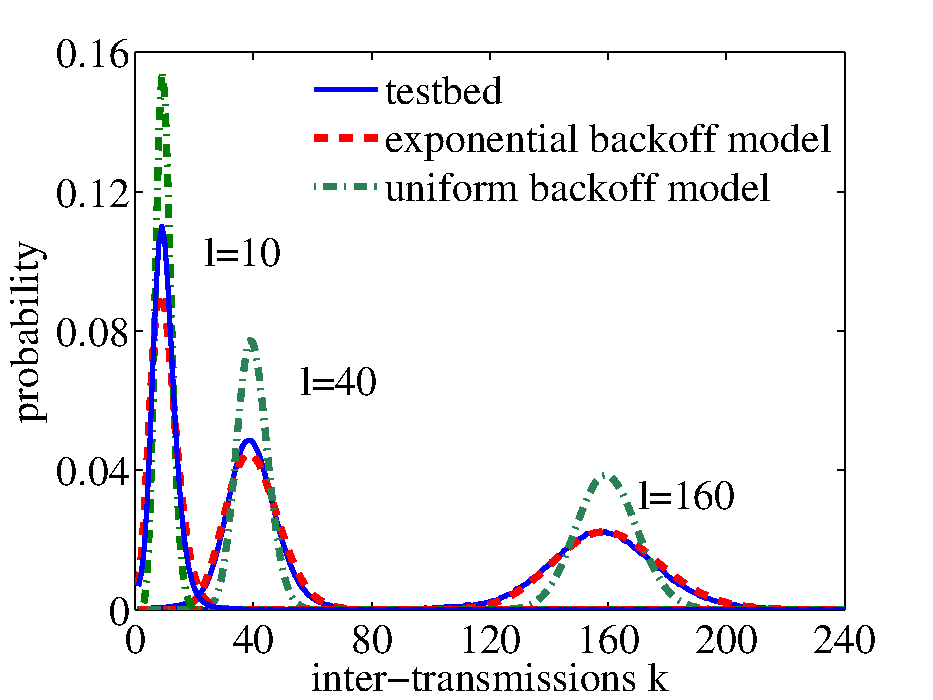
\includegraphics[width=\linewidth]{gfx/examples/pdf_gaus_vs_uni_vs_10_40_160}  
    \caption{Minipage-Grafik Nummer zwei}
    \label{fig:chapter03:minipage:grafik2}
  \end{minipage}
\end{figure}

In vitae est eget velit mattis lobortis. In hac habitasse platea dictumst. Quisque aliquam quam et justo pellentesque ullamcorper. Curabitur elementum mattis leo facilisis tincidunt. Fusce posuere viverra ultricies. Cras eget velit et ipsum gravida imperdiet et hendrerit orci.

Maecenas fringilla viverra urna ut egestas. Nulla sagittis molestie libero eget luctus. Nulla non odio sit amet magna vehicula tincidunt. Nulla accumsan ornare placerat. In posuere scelerisque quam, sed posuere urna eleifend quis. Pellentesque sed quam quis dui vulputate convallis ut ac diam. In hac habitasse platea dictumst. Donec molestie auctor dapibus. Vivamus in erat risus, ut aliquet diam. Duis vel velit ante, id ullamcorper turpis. Lorem ipsum dolor sit amet, consectetur adipiscing elit. In accumsan ornare tellus a porttitor. Etiam facilisis dui et sem eleifend id luctus nisl scelerisque. Aenean quis commodo libero. Nulla quis semper dolor. 

%
% Section: Tabellen 
%
\section{Tabellen}
\label{sec:chapter03:tabellen}
Sed lobortis vestibulum euismod. Vivamus vestibulum gravida nisi vitae condimentum. Nullam nec lacus nibh. Phasellus arcu magna, varius eget viverra a, elementum eu dolor. Aliquam erat volutpat. Sed nibh leo, vestibulum quis lacinia in, vestibulum sollicitudin nulla. In iaculis, purus in imperdiet sagittis, tortor diam pellentesque lectus, eget faucibus ante elit at tortor.

%
% Section: Listings 
%
\section{Listings}
\label{sec:chapter03:listings}
Aliquam ut pretium lectus. Curabitur in eros et sapien aliquet luctus ut sit amet eros. Proin et libero non mi venenatis aliquet at sed lorem. Ut sed enim mi, id viverra eros. Cras metus ante, placerat id commodo at, molestie non libero. Aenean eu risus erat, vel consequat metus. Sed malesuada metus sit amet nisl viverra hendrerit.


%
% Section: Equations
%
\section{Equations}
\label{sec:chapter03:equations}
Pellentesque sed quam quis dui vulputate convallis ut ac diam. In hac habitasse platea dictumst. Donec molestie auctor dapibus. Vivamus in erat risus, ut aliquet diam. Duis vel velit ante, id ullamcorper turpis.
%
\begin{equation}
 U = R * I
\end{equation}

Lorem ipsum dolor sit amet, consectetur adipiscing elit. In accumsan ornare tellus a porttitor. Etiam facilisis dui et sem eleifend id luctus nisl scelerisque. Aenean quis commodo libero. Nulla quis semper dolor.
%
\begin{equation}
 I = \frac{U}{R} 
\end{equation}

In the following we use probability theory to derive closed-form expressions for the fairness that is achieved among $M$ contending stations. We tag station $M$ and denote $K_i$ the inter-transmissions of station $i = 1 \dots M-1$ and let $K = \sum_{i=1}^{M-1} K_i$. The conditional probability $P[K\!=\!k|l]$ can be defined for $M \ge 2$ as
%
\begin{equation}
\mathsf{P}[K\!=\!k|l] = \mathsf{P} \Biggl[\sum_{i=1}^{M-1} K_i = k \Big| l \Biggr]
\label{eq:chapter03:exactpmf}
\end{equation}
%
where the random variables $K_i$ are the integers that satisfy
%
\begin{equation*}
\sum_{j=1}^{K_i} b_i(j) \le \sum_{j=1}^{l} b_M(j) \;\;\; \textmd{and} \;\;\; \sum_{j=1}^{K_i+1} b_i(j) > \sum_{j=1}^{l} b_M(j) .
\end{equation*}


%
% Section: Theorem and Proof
%
\section{Theorem and Proof}
\label{sec:chapter03:theorem}
We use the central limit theorem to derive the long-term fairness. In the sequel, we denote normal random variables $N(\mu,\sigma^2)$ where $\mu$ is the mean and $\sigma^2$ the variance.
%
\begin{Theorem}[Gaussian approximation]
\label{th:chapter03:twostationsgaussian}
%
Let the $b_i(j)$ be i.i.d. random variables with mean $\mu$ and variance $\sigma^2$ and let $M=2$. For $k,l \gg 1$ (\ref{eq:chapter03:exactpmf}) is approximately Gaussian where
%
\begin{equation*}
\mathsf{P}[K \!\le\! k|l] \approx \mathsf{P}\biggl[ N(0,1) \le \frac{\mu\,(k-l)}{\sigma\,\sqrt{k+l}} \biggr] .
\end{equation*}
%
\end{Theorem}
%
\begin{proof}
%
For $M=2$ we have from (\ref{eq:chapter03:exactpmf}) that
%
\begin{equation*}
\mathsf{P}[K \!<\! k|l] = \mathsf{P} \Biggl[\, \sum_{j=1}^k b_1(j) > \sum_{j=1}^l b_2(j) \Biggr]
\end{equation*}
%
and after expansion and some normalization this equals
%
\begin{equation*}
= \mathsf{P}\Biggl[ \frac{\sum_{j=1}^{l}b_2(j) - l\mu}{\sigma\sqrt{l}} - \frac{\sum_{j=1}^{k}b_1(j) - k\mu}{\sigma\sqrt{l}} < \frac{\mu(k-l)}{\sigma\sqrt{l}} \Biggr].
\end{equation*}
%
Using the central limit theorem it follows that
%
\begin{equation*}
\mathsf{P}[K \!<\! k|l] \approx \mathsf{P} \biggl[ N(0,1) - N \biggl(0,\frac{k}{l}\biggr) < \frac{\mu(k-l)}{\sigma\sqrt{l}} \biggr] .
\end{equation*}
%
Since the normal distribution with zero mean is symmetric we can replace the subtraction of $N(0,k/l)$ by addition. Furthermore, the sum of two normal random variables $N(\mu_1, \sigma_1^2)$ and $N(\mu_2, \sigma_2^2)$ is normal with $N(\mu_1+\mu_2, \sigma_1^2+ \sigma_2^2)$ such that
%
\begin{equation*}
\mathsf{P}[K \!<\! k|l] \approx \mathsf{P} \biggl[ N\biggl(0,\frac{k+l}{l}\biggr) < \frac{\mu(k-l)}{\sigma\sqrt{l}} \biggr] .
\end{equation*}
%
Finally, we use that if $X$ is $N(a\mu,a^2\sigma^2)$ then $Y = X/a$ is $N(\mu,\sigma^2)$ with $a^2 = (k+l)/l$ to standardize the result.
%
\end{proof}

Th. \ref{th:chapter03:twostationsgaussian} assumes i.i.d. random countdown values. It does, however, not make any assumption about their distribution.

%*************************************************************************
% Backmatter
%*************************************************************************
\appendix
%\renewcommand{\thechapter}{\alph{chapter}}
\cleardoublepage
\part{Anhang}
% %************************************************
\chapter{Introduction to the ClassicThesis style}\label{ch:classicthesis}
%************************************************
The ClassicThesis bundle for \LaTeX\ has two goals:
\begin{enumerate}
    \item Provide students with an easy-to-use template for their
    Master's
    or PhD thesis. (Though it might also be used by other types of
    authors
    for reports, books, etc.)
    \item Provide a classic, high-quality typographic style that is
    inspired by \citeauthor{bringhurst:2002}'s ``\emph{The Elements of
    Typographic Style}'' \citep{bringhurst:2002}.
    \marginpar{\myTitle \myVersion}
\end{enumerate}
The bundle is configured to run with a \emph{full}
MiK\TeX\ or \TeX Live\footnote{See the file \texttt{LISTOFFILES} for
needed packages. Furthermore, \texttt{classicthesis}
works with most other distributions and, thus, with most systems
\LaTeX\ is available for.}
installation right away and, therefore, it uses only freely available
fonts. (Minion fans can easily adjust the style to their needs.)

People interested only in the nice style and not the whole bundle can
now use the style stand-alone via the file \texttt{classicthesis.sty}.
This works now also with ``plain'' \LaTeX.

As of version 3.0, \texttt{classicthesis} can also be easily used with
\mLyX\footnote{\url{http://www.lyx.org}} thanks to Nicholas Mariette
and Ivo Pletikosić. The \mLyX\ version of this manual will contain
more information on the details.

This should enable anyone with a basic knowledge of \LaTeXe\ or \mLyX\ to
produce beautiful documents without too much effort. In the end, this
is my overall goal: more beautiful documents, especially theses, as I
am tired of seeing so many ugly ones.

The whole template and the used style is released under the
\acsfont{GNU} General Public License.

If you like the style then I would appreciate a postcard:
\begin{center}
    André Miede \\
    Detmolder Straße 32 \\
    31737 Rinteln \\
    Germany
\end{center}
The postcards I received so far are available at:
\begin{center}
    \url{http://postcards.miede.de}
\end{center}
\marginpar{A well-balanced line width improves the legibility of
the text. That's what typography is all about, right?}
So far, many theses, some books, and several other publications have
been typeset successfully with it. If you are interested in some
typographic details behind it, enjoy Robert Bringhurst's wonderful book.
% \citep{bringhurst:2002}.

\paragraph{Important Note:} Some things of this style might look
unusual at first glance, many people feel so in the beginning.
However, all things are intentionally designed to be as they are,
especially these:
\begin{itemize}
    \item No bold fonts are used. Italics or spaced small caps do the
    job quite well.
    \item The size of the text body is intentionally shaped like it
    is. It supports both legibility and allows a reasonable amount of
    information to be on a page. And, no: the lines are not too short.
    \item The tables intentionally do not use vertical or double
    rules. See the documentation for the \texttt{booktabs} package for
    a nice discussion of this topic.\footnote{To be found online at
    \url{http://mirror.ctan.org/macros/latex/contrib/booktabs/}.}
    \item And last but not least, to provide the reader with a way
    easier access to page numbers in the table of contents, the page
    numbers are right behind the titles. Yes, they are \emph{not}
    neatly aligned at the right side and they are \emph{not} connected
    with dots that help the eye to bridge a distance that is not
    necessary. If you are still not convinced: is your reader
    interested in the page number or does she want to sum the numbers
    up?
\end{itemize}
Therefore, please do not break the beauty of the style by changing
these things unless you really know what you are doing! Please.

\paragraph{Yet Another Important Note:} Since \texttt{classicthesis}'
first release in 2006, many things have changed in the \LaTeX\ world.
Trying to keep up-to-date, \texttt{classicthesis} grew and evolved
into many directions, trying to stay (some kind of) stable and be
compatible with its port to \mLyX. However, there are still many
remains from older times in the code, many dirty workarounds here and
there, and several other things I am absolutely not proud of (for
example my unwise combination of \acsfont{KOMA} and
\texttt{titlesec} etc.).
\graffito{An outlook into the future of \texttt{classicthesis}.}

Currently, I am looking into how to completely re-design and
re-implement \texttt{classicthesis} making it easier to maintain and
to use. As a general idea, \texttt{classicthesis.sty} should be
developed and distributed separately from the template bundle itself.
Excellent spin-offs such as \texttt{arsclassica} could also be
integrated (with permission by their authors) as format configurations.
Also, current trends of \texttt{microtype}, \texttt{fontspec}, etc.
should be included as well. As I am not really into deep
\LaTeX\ programming,
I will reach out to the \LaTeX\ community for their expertise and help.


\section{Organization}
A very important factor for successful thesis writing is the
organization of the material. This template suggests a structure as
the following:
\begin{itemize}
    \marginpar{You can use these margins for summaries of the text
    body\dots}
    \item\texttt{Chapters/} is where all the ``real'' content goes in
    separate files such as \texttt{Chapter01.tex} etc.
    % \item\texttt{Examples/} is where you store all listings and other
    % examples you want to use for your text.
    \item\texttt{FrontBackMatter/} is where all the stuff goes that
    surrounds the ``real'' content, such as the acknowledgments,
    dedication, etc.
    \item\texttt{gfx/} is where you put all the graphics you use in
    the thesis. Maybe they should be organized into subfolders
    depending on the chapter they are used in, if you have a lot of
    graphics.
    \item\texttt{Bibliography.bib}: the Bib\TeX\ database to organize
    all the references you might want to cite.
    \item\texttt{classicthesis.sty}: the style definition to get this
    awesome look and feel. Does not only work with this thesis template
    but also on its own (see folder \texttt{Examples}). Bonus: works
    with both \LaTeX\ and \textsc{pdf}\LaTeX\dots and \mLyX.
    % \item\texttt{ClassicThesis.tcp} a \TeX nicCenter project file.
    Great tool and it's free!
    \item\texttt{ClassicThesis.tex}: the main file of your thesis
    where all gets bundled together.
    \item\texttt{classicthesis-config.tex}: a central place to load all
    nifty packages that are used. % In there, you can also activate
    % backrefs in order to have information in the bibliography about
    % where a source was cited in the text (\ie, the page number).

    \emph{Make your changes and adjustments here.} This means that you
    specify here the options you want to load \texttt{classicthesis.sty}
    with. You also adjust the title of your thesis, your name, and all
    similar information here. Refer to \autoref{sec:custom} for more
    information.

    This had to change as of version 3.0 in order to enable an easy
    transition from the ``basic'' style to \mLyX.
\end{itemize}
In total, this should get you started in no time.


\clearpage
\section{Style Options}\label{sec:options}
There are a couple of options for \texttt{classicthesis.sty} that
allow for a bit of freedom concerning the layout:
\marginpar{\dots or your supervisor might use the margins for some
    comments of her own while reading.}
\begin{itemize}
    \item General:
        \begin{itemize}
            \item\texttt{drafting}: prints the date and time at the bottom of
            each page, so you always know which version you are dealing with.
            Might come in handy not to give your Prof. that old draft.
        \end{itemize}

    \item Parts and Chapters:
        \begin{itemize}
            \item\texttt{parts}: if you use Part divisions for your document,
            you should choose this option. (Cannot be used together with
            \texttt{nochapters}.)

            \item\texttt{linedheaders}: changes the look of the chapter
            headings a bit by adding a horizontal line above the chapter
            title. The chapter number will also be moved to the top of the
            page, above the chapter title.
        \end{itemize}

    \item Typography:
        \begin{itemize}
            \item\texttt{eulerchapternumbers}: use figures from Hermann Zapf's
            Euler math font for the chapter numbers. By default, old style
            figures from the Palatino font are used.

            \item\texttt{beramono}: loads Bera Mono as typewriter font.
            (Default setting is using the standard CM typewriter font.)

            \item\texttt{eulermath}: loads the awesome Euler fonts for math.
            Pala\-tino is used as default font.
        \end{itemize}

    \marginpar{Options are enabled via \texttt{option=true}}

    \item Table of Contents:
        \begin{itemize}
            \item\texttt{tocaligned}: aligns the whole table of contents on
            the left side. Some people like that, some don't.

            \item\texttt{dottedtoc}: sets pagenumbers flushed right in the
            table of contents.

            \item\texttt{manychapters}: if you need more than nine chapters for
            your document, you might not be happy with the spacing between the
            chapter number and the chapter title in the Table of Contents.
            This option allows for additional space in this context.
            However, it does not look as ``perfect'' if you use
            \verb|\parts| for structuring your document.
        \end{itemize}

    \item Floats:
        \begin{itemize}
            \item\texttt{listings}: loads the \texttt{listings} package (if not
            already done) and configures the List of Listings accordingly.

            \item\texttt{floatperchapter}: activates numbering per chapter for
            all floats such as figures, tables, and listings (if used).
        \end{itemize}

\end{itemize}

Furthermore, pre-defined margins for different paper sizes are available, \eg, \texttt{a4paper}, \texttt{a5paper}, and \texttt{letterpaper}. These are based on your chosen option of \verb|\documentclass|.

The best way to figure these options out is to try the different
possibilities and see what you and your supervisor like best.

In order to make things easier, \texttt{classicthesis-config.tex}
contains some useful commands that might help you.


\section{Customization}\label{sec:custom}
%(As of v3.0, the Classic Thesis Style for \LaTeX{} and \mLyX{} share
%the same two \texttt{.sty} files.)
This section will show you some hints how to adapt
\texttt{classicthesis} to your needs.

The file \texttt{classicthesis.sty}
contains the core functionality of the style and in most cases will
be left intact, whereas the file \texttt{classic\-thesis-config.tex}
is used for some common user customizations.

The first customization you are about to make is to alter the document
title, author name, and other thesis details. In order to do this, replace
the data in the following lines of \texttt{classicthesis-config.tex:}%
\marginpar{Modifications in \texttt{classic\-thesis-config.tex}%
}

\begin{lstlisting}
    % **************************************************
    % 2. Personal data and user ad-hoc commands
    % **************************************************
    \newcommand{\myTitle}{A Classic Thesis Style\xspace}
    \newcommand{\mySubtitle}{An Homage to...\xspace}
\end{lstlisting}

Further customization can be made in \texttt{classicthesis-config.tex}
by choosing the options to \texttt{classicthesis.sty}
(see~\autoref{sec:options}) in a line that looks like this:

\begin{lstlisting}
  \PassOptionsToPackage{
    drafting=true,    % print version information on the bottom of the pages
    tocaligned=false, % the left column of the toc will be aligned (no indentation)
    dottedtoc=false,  % page numbers in ToC flushed right
    parts=true,       % use part division
    eulerchapternumbers=true, % use AMS Euler for chapter font (otherwise Palatino)
    linedheaders=false,       % chaper headers will have line above and beneath
    floatperchapter=true,     % numbering per chapter for all floats (i.e., Figure 1.1)
    listings=true,    % load listings package and setup LoL
    subfig=true,      % setup for preloaded subfig package
    eulermath=false,  % use awesome Euler fonts for mathematical formulae (only with pdfLaTeX)
    beramono=true,    % toggle a nice monospaced font (w/ bold)
    minionpro=false   % setup for minion pro font; use minion pro small caps as well (only with pdfLaTeX)
  }{classicthesis}
\end{lstlisting}

Many other customizations in \texttt{classicthesis-config.tex} are
possible, but you should be careful making changes there, since some
changes could cause errors.

% Finally, changes can be made in the file \texttt{classicthesis.sty},%
% \marginpar{Modifications in \texttt{classicthesis.sty}%
% } although this is mostly not designed for user customization. The
% main change that might be made here is the text-block size, for example,
% to get longer lines of text.


\section{Issues}\label{sec:issues}
This section will list some information about problems using
\texttt{classic\-thesis} in general or using it with other packages.

Beta versions of \texttt{classicthesis} can be found at Bitbucket:
\begin{center}
    \url{https://bitbucket.org/amiede/classicthesis/}
\end{center}
There, you can also post serious bugs and problems you encounter.


\section{Future Work}
So far, this is a quite stable version that served a couple of people
well during their thesis time. However, some things are still not as
they should be. Proper documentation in the standard format is still
missing. In the long run, the style should probably be published
separately, with the template bundle being only an application of the
style. Alas, there is no time for that at the moment\dots it could be
a nice task for a small group of \LaTeX nicians.

Please do not send me email with questions concerning \LaTeX\ or the
template, as I do not have time for an answer. But if you have
comments, suggestions, or improvements for the style or the template
in general, do not hesitate to write them on that postcard of yours.


\section{Beyond a Thesis}
The layout of \texttt{classicthesis.sty} can be easily used without the
framework of this template. A few examples where it was used to typeset
an article, a book or a curriculum vitae can be found in the folder
\texttt{Examples}. The examples have been tested with
\texttt{latex} and \texttt{pdflatex} and are easy to compile. To
encourage you even more, PDFs built from the sources can be found in the
same folder.


\section{License}
\paragraph{GNU General Public License:} This program is free software;
you can redistribute it and/or modify
it under the terms of the \acsfont{GNU} General Public License as
published by
the Free Software Foundation; either version 2 of the License, or
(at your option) any later version.

This program is distributed in the hope that it will be useful,
but \emph{without any warranty}; without even the implied warranty of
\emph{merchant\-ability} or \emph{fitness for a particular purpose}.
See the
\acsfont{GNU} General Public License for more details.

You should have received a copy of the \acsfont{GNU} General
Public License
along with this program; see the file \texttt{COPYING}.  If not,
write to
the Free Software Foundation, Inc., 59 Temple Place - Suite 330,
Boston, MA 02111-1307, USA.

\paragraph{classichthesis Authors' note:} There have been some discussions about the GPL's implications on using \texttt{classicthesis} for theses etc. Details can be found here:
\begin{center}
  \url{https://bitbucket.org/amiede/classicthesis/issues/123/}
\end{center}

We chose (and currently stick with) the GPL because we would not like to compete with proprietary modified versions of our own work. However, the whole template is free as free beer and free speech. We will not demand the sources for theses, books, CVs, etc. that were created using \texttt{classicthesis}.

Postcards are still highly appreciated.





%*****************************************
%*****************************************
%*****************************************
%*****************************************
%*****************************************

% %********************************************************************
% Appendix
%*******************************************************
% If problems with the headers: get headings in appendix etc. right
%\markboth{\spacedlowsmallcaps{Appendix}}{\spacedlowsmallcaps{Appendix}}
\chapter{Appendix Test}
Lorem ipsum at nusquam appellantur his, ut eos erant homero
concludaturque. Albucius appellantur deterruisset id eam, vivendum
partiendo dissentiet ei ius. Vis melius facilisis ea, sea id convenire
referrentur, takimata adolescens ex duo. Ei harum argumentum per. Eam
vidit exerci appetere ad, ut vel zzril intellegam interpretaris.
\graffito{More dummy text.}

%Errem omnium ea per, pro congue populo ornatus cu, ex qui dicant
%nemore melius. No pri diam iriure euismod. Graecis eleifend
%appellantur quo id. Id corpora inimicus nam, facer nonummy ne pro,
%kasd repudiandae ei mei. Mea menandri mediocrem dissentiet cu, ex
%nominati imperdiet nec, sea odio duis vocent ei. Tempor everti
%appareat cu ius, ridens audiam an qui, aliquid admodum conceptam ne
%qui. Vis ea melius nostrum, mel alienum euripidis eu.

\section{Appendix Section Test}
Test: \autoref{tab:moreexample} (This reference should have a
lowercase, small caps \spacedlowsmallcaps{A} if the option
\texttt{floatperchapter} is activated, just as in the table itself
 $\rightarrow$ however, this does not work at the moment.)

\begin{table}[h]
    \myfloatalign
    \begin{tabularx}{\textwidth}{Xll} \toprule
        \tableheadline{labitur bonorum pri no} & \tableheadline{que vista}
        & \tableheadline{human} \\ \midrule
        fastidii ea ius & germano &  demonstratea \\
        suscipit instructior & titulo & personas \\
        %postulant quo & westeuropee & sanctificatec \\
        \midrule
        quaestio philosophia & facto & demonstrated \\
        %autem vulputate ex & parola & romanic \\
        %usu mucius iisque & studio & sanctificatef \\
        \bottomrule
    \end{tabularx}
    \caption[Autem usu id]{Autem usu id.}
    \label{tab:moreexample}
\end{table}

%Nulla fastidii ea ius, exerci suscipit instructior te nam, in ullum
%postulant quo. Congue quaestio philosophia his at, sea odio autem
%vulputate ex. Cu usu mucius iisque voluptua. Sit maiorum propriae at,
%ea cum primis intellegat. Hinc cotidieque reprehendunt eu nec. Autem
%timeam deleniti usu id, in nec nibh altera.




\section{Another Appendix Section Test}
Equidem detraxit cu nam, vix eu delenit periculis. Eos ut vero
constituto, no vidit propriae complectitur sea. Diceret nonummy in
has, no qui eligendi recteque consetetur. Mel eu dictas suscipiantur,
et sed placerat oporteat. At ipsum electram mei, ad aeque atomorum
mea. There is also a useless Pascal listing below: \autoref{lst:useless}.

\begin{lstlisting}[float=b,language=Pascal,frame=tb,caption={A floating example (\texttt{listings} manual)},label=lst:useless]
for i:=maxint downto 0 do
begin
{ do nothing }
end;
\end{lstlisting}

%Ei solet nemore consectetuer nam. Ad eam porro impetus, te choro omnes
%evertitur mel. Molestie conclusionemque vel at, no qui omittam
%expetenda efficiendi. Eu quo nobis offendit, verterem scriptorem ne
%vix.


\chapter{Liste der relevanten Durchführungsverordnungen}
\label{extra_implementing_regulations}

\begin{center}
    \footnotesize
    Namen der Verordnungen sinnesgemäß gekürzt. \\
    Stand 2023 (\textdagger Außer Kraft)
\end{center}

% Regulation 549/2004 SES Framework
\section{Rahmenverordnung}

    Auf Basis der \vo{VO}{EG}{549/2004} verfasst:

    \begin{itemize}
        \item \vo{DVO}{EU}{390/2013}\textdagger: Leistungssystem für \acs{ANS} und \acs{NF}
        \item \vo{DVO}{EU}{2019/317}: Leistungssystem und Gebührenregelung in \ac{SES}
        \item \vo{DVO}{EU}{2020/1627}: Sondermaßnahmen aufgrund von COVID-19 
    \end{itemize}

% Regulation 550/2004 Provision of Air Navigation Services in SES
\section{ANS Bereitstellung} 
    Auf Basis der \vo{VO}{EG}{550/2004} verfasst:

    \begin{itemize}
        \item \vo{DVO}{EU}{176/2011}: Informationen zur Einrichtung eines \acs{FAB}
        \item \vo{DVO}{EU}{391/2013}\textdagger: Gebührenregelung für Flugsicherungsdienste
        \item \vo{DVO}{EU}{409/2013}: ,,\acs{ATM} Master Plan``
        \item \vo{DVO}{EU}{448/2014}\textdagger: Änderung der \vo{DVO}{EU}{1035/2011}
        \item \vo{DVO}{EU}{716/2014}\textdagger: Pilotvorhaben zum \acs{ATM} Master Plan
    \end{itemize}

\section{Luftraumnutzung und -organisation} 
% Regulation 551/2004 Organisation and Use of the Airspace in SES
    Auf Basis der \vo{VO}{EG}{551/2004} verfasst:

    \begin{itemize}
        \item \vo{DVO}{EU}{2150/2005}: Regeln zur \ac{FUA}
        \item \vo{DVO}{EU}{255/2010}: Regeln zu Verkehrsflussregelung (\acs{ATFM})
        \item Entscheidung\footnote{der Kommission vom 07.07.2011} zur Benennung des \acf{NM} für \ac{ATM}-\acs{NF}
        \item \vo{DVO}{EU}{677/2011}\textdagger: Implementation von \ac{ATM}-\ac{NF}
        \item \vo{DVO}{EU}{970/2014}: Implementation von \ac{ATM}-\acs{NF}
        \item \vo{DVO}{EU}{2016/1006}: Anpassung der \vo{DVO}{EU}{255/2010} an \acs{ICAO}  %  as regards ICAO provisions
        \item \vo{DVO}{EU}{2016/2345}: Anpassung der \vo{DVO}{EU}{262/2009} et al. an \acs{ICAO}  %  and 1079/2012 as regards references to ICAO provisions
        \item \vo{DVO}{EU}{2017/2159}: Anpassung der \vo{DVO}{EU}{255/2010} an \acs{ICAO}  %  as regards references to ICAO provisions
        \item \vo{DVO}{EU}{2017/2160}: Anpassung der \vo{DVO}{EU}{1079/2012} an \acs{ICAO} %  as regards references to ICAO provisions
        \item \vo{DVO}{EU}{2019/123}: Implementation von \ac{ATM}-\ac{NF}
        \item Durchführungsbeschluss (\acs{EU}) 2019/709: Benennung des \ac{NM} 
    \end{itemize}

% Regulation 552/2004 Interoperability of the European ATM Network
\section{Interoperabilität} 
    Auf Basis der \vo{VO}{EG}{552/2004} verfasst:

    \begin{itemize}
        \item \vo{DVO}{EU}{1032/2006}:  Austausch von Flugdaten zwischen \acp{ATC} % Exchange of Flight Data Between ATC Units
        \item \vo{DVO}{EU}{1033/2006}:  Flugplanverfahren während Pre-Flight Phase % Procedures for Flight Plans in the Pre-Flight Phase
        \item \vo{DVO}{EU}{633/2007}:   \acf{FMTP} % Flight Message Transfer Protocol for Use by ATC Units
        \item \vo{DVO}{EU}{29/2009}:    \acf{DLS} % Data link services for the SES
        \item \vo{DVO}{EU}{30/2009}:    Automatisierungsanforderungen an \ac{DLS} % Requirements for Automatic Systems for the Exchange of Flight Data Supporting Data Link Services
        \item \vo{DVO}{EU}{262/2009}:   Benutzung der Mode S Codes % Allocation and Use of Mode S Interrogator Codes
        \item \vo{DVO}{EU}{73/2010}:    Qualität von Luftlagedaten % Quality of Aeronautical Data and Aeronautical Information
        \item \vo{DVO}{EU}{1206/2011}:  Anforderungen der Flugzeugidentifikation % Requirements on Aircraft Identification for Surveillance of the SES
        \item \vo{DVO}{EU}{1207/2011}:  Leistungsanforderungen an \ac{SUR} % Requirements for the performance and the interoperability of surveillance for the SES
        \item \vo{DVO}{EU}{1079/2012}:  Anforderungen der Sprachkanalabstände % Requirements for Voice Channels Spacing for the SES
        \item \vo{DVO}{EU}{428/2013}:   Anpassung der \vo{DVO}{EU}{1033/2006} an \acs{ICAO} Art.3(1)% amending Regulation 1033/2006 as regards the ICAO provisions referred to in Article 3(1)
        \item \vo{DVO}{EU}{657/2013}:   Anforderungen an Sprachkanalabstände % Requirements for Voice Channels Spacing for the SES
        \item \vo{DVO}{EU}{441/2014}:   Anforderungen an \acf{DLS} % Requirements on Data Link Services for the SES
        \item \vo{DVO}{EU}{1028/2014}:  Interoperabilitätsanfoderungen an \acs{SUR} % Requirements for the Performance and the Interoperability of Surveillance for the SES
        \item \vo{DVO}{EU}{1029/2014}:  Qualitätsanforderungen an Luftlagedaten % Requirements on the Quality of Aeronautical Data and Aeronautical Information for the SES
        \item \vo{DVO}{EU}{310/2015}:   Änderung der \vo{DVO}{EU}{29/2009} bzgl. \acs{DLS} % amending Regulation  on data link services for the SES
        \item \vo{DVO}{EU}{2016/2120}:  Änderung der \vo{DVO}{EU}{1033/2006} % amending Regulation  as regards the provisions
        \item \vo{DVO}{EU}{2017/386}:   Interoperabilitätsanfoderungen an \acs{SUR} % Requirements for the Performance and the Interoperability of Surveillance for the SES
        \item \vo{DVO}{EU}{2018/139}:   Anpassung der \vo{DVO}{EU}{1033/2006} an {ICAO} % amending Regulation  as regards references to ICAO provisions
        \item \vo{DVO}{EU}{2019/1070}:  Änderung der \vo{DVO}{EU}{29/2009} bzgl. \acs{DLS}% amending Regulation  on data link services for the SES
        \item \vo{DVO}{EU}{2020/208}:   Änderung der \vo{DVO}{EU}{29/2009} bzgl. \acs{DLS}% amending Regulation  on data link services for the SES
        \item \vo{DVO}{EU}{2020/587}:   Änderung der \vo{DVO}{EU}{1206f./2011} % amending Regulation  and Regulation No 1207/2011
    \end{itemize}

\pagebreak   
% Regulation 2018/1139 Common Rules in the Field of Civil Aviation and Establishing EASA
\section{Einheitliche Regelung der Zivilluftfahrt} 
    Auf Basis der \vo{VO}{EU}{2018/1139} verfasst:

    \begin{itemize}
        \item \vo{DVO}{EU}{2021/1338} % amending Regulation 2017/373 as regards reporting between organizations and requirements for meteorological services
        \item \vo{DVO}{EU}{2020/1177} % amending Regulation 2020/469 by postponing dates due to COVID-19
        \item \vo{DVO}{EU}{2020/746} % amending Regulation No 2019/947 due to COVID-19
        \item \vo{DVO}{EU}{2020/639} % amending Regulation No 2019/947 with scenarios for operations beyond VLOS
        \item \vo{DVO}{EU}{2020/469} % amending Regulations 923/2012, 139/2014 and 2017/373 and repealing Regulation 73/2010
        \item \vo{DVO}{EU}{2019/945} % UAS and third-country operators of UAS
        \item \vo{DVO}{EU}{2019/947} % rules and procedures for unmanned aircraft
        \item \vo{DVO}{EU}{2018/1048} % Airspace Usage Requirements and Operating Procedures Concerning PBN
        \item \vo{DVO}{EU}{2017/373} % Requirements for Providers of ATM/ANS and other ATM Network Functions and their Oversight
        \item \vo{DVO}{EU}{2016/1185} % amending Regulation 923/2012 as regards the update of SERA
        \item \vo{DVO}{EU}{2016/583} % amending Regulation 1332/2011 for airborne collision avoidance
        \item \vo{DVO}{EU}{2015/340} % Requirements and Procedures Relating to ATCO Licences
        \item \vo{DVO}{EU}{923/2012} % Common Rules of the Air and Operational Provisions Regarding Services and Procedures in Air Navigation
        \item \vo{DVO}{EU}{1332/2011} % Common Airspace Usage Requirements and Operating Procedures for Airborne Collision Avoidance
    \end{itemize}
\chapter{Interne Anweisungen Definitionen}

\section{Betriebliche Anweisung: Technik}
\label{ba_technik}

jhfjiashfjkshdkjfhsjkdf


\section{Fachliche Anweisung: Freigaben}
\label{fa_freigaben}

uashzdkjashdjkahsdkajsh 




\chapter{Liste der Anforderungen für die Impactanalyse}



\chapter{Referenzen zur Datenquelle 1}
    
    \section{Darstellung der Gesetzgebungsprozesse der EU}
    
    \begin{figure}[H]
        \centering
        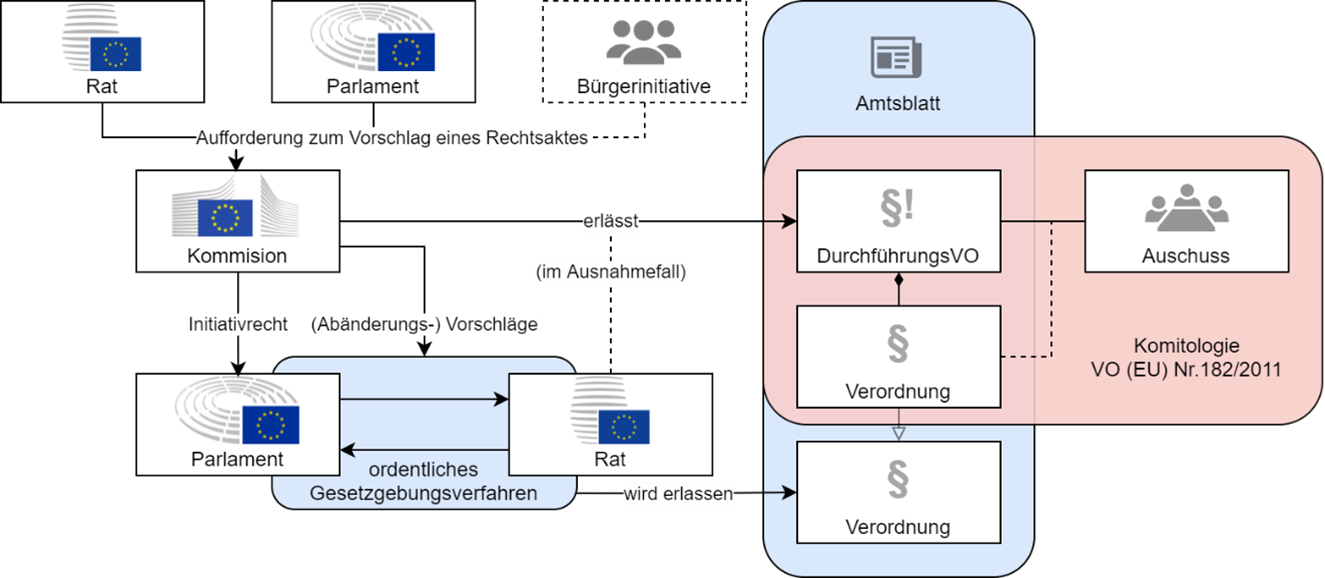
\includegraphics[width=\linewidth]{gfx/Gesegebungsprozess.png}
        \caption{Gesetzgebungsprozess der EU} 
        [Eigene Darstellung]
        \label{fig:europeg}
    \end{figure}

\section{Semantic Web Tech-Stack}
    
    \begin{figure}[H]
        \centering
        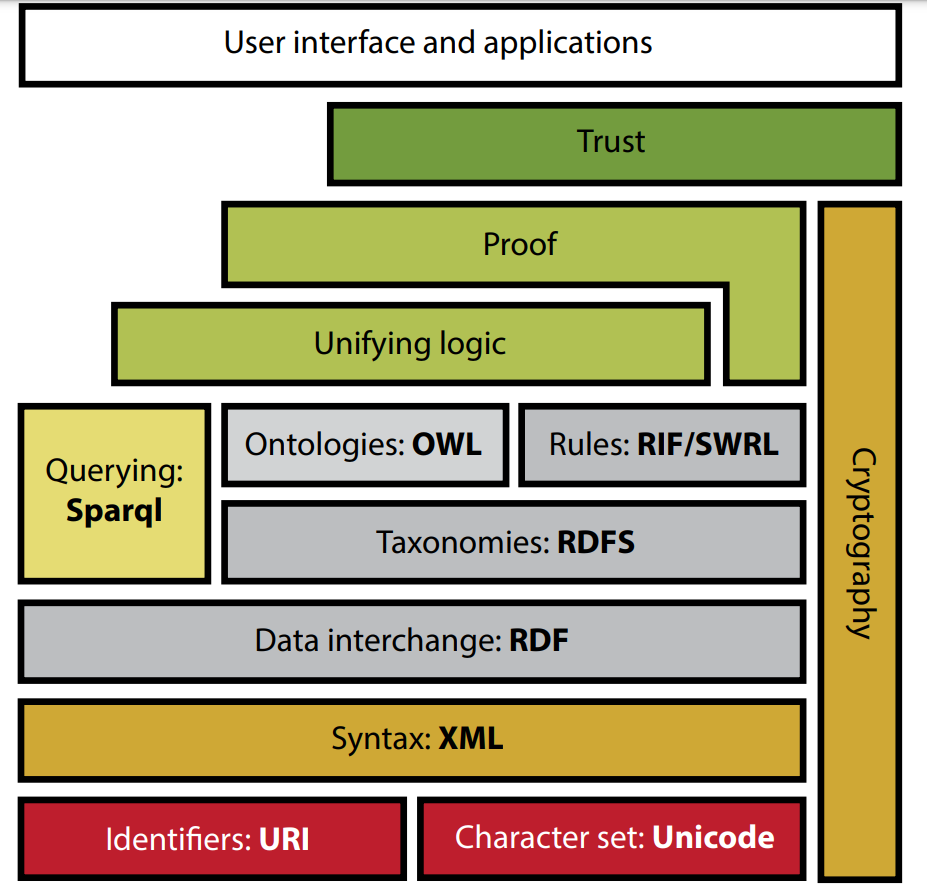
\includegraphics[width=.75\linewidth]{gfx/semantic_web_cake.png}
        \caption{Semantic Web Tech-Stack}\cite[10]{eu_cellar}\footnote{Ursprüngliche Quelle nach 2014 nicht mehr verfügbar}
        \label{fig:semantic}
    \end{figure}


\begin{lstlisting}[language=XML]
    <ANNOTATION>
        <TYPE_OF_LINK_TARGET>MS</TYPE_OF_LINK_TARGET>
        <ROLE2>{R|http://publications.europa.eu/resource/authority/fd_375/R}<ROLE2>
        <START_OF_VALIDITY>2020-11-05</START_OF_VALIDITY>
        <REFERENCE_TO_MODIFIED_LOCATION>
            {AN|http://publications.europa.eu/resource/authority/fd_370/AN} V
            {PO|http://publications.europa.eu/resource/authority/fd_370/PO} MET
            {PTA|http://publications.europa.eu/resource/authority/fd_370/PTA} (c) PT 1
        </REFERENCE_TO_MODIFIED_LOCATION>
    </ANNOTATION>
\end{lstlisting}


    % \begin{figure}
    %     \centering
    %     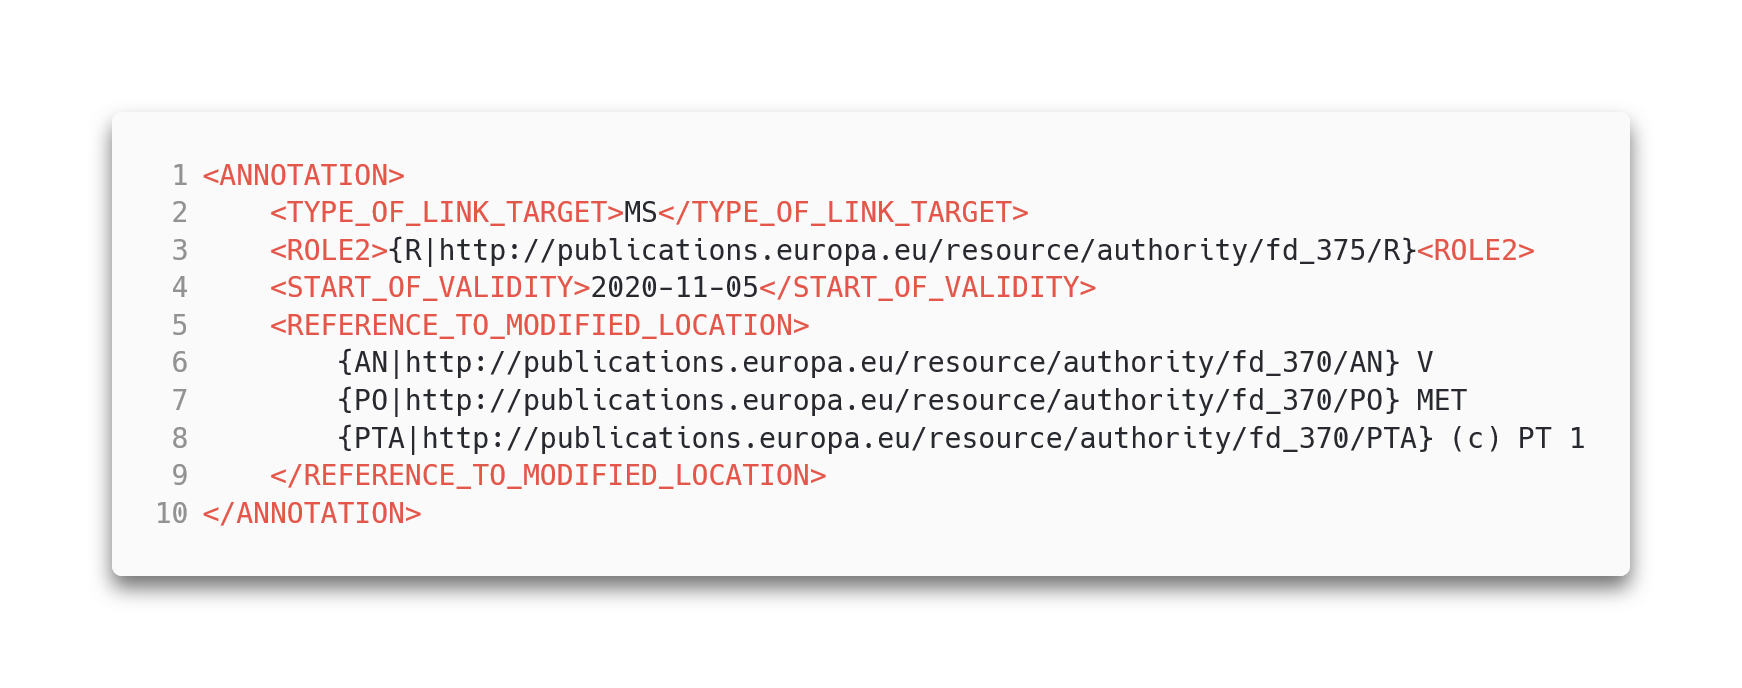
\includegraphics[width=\linewidth]{gfx/anno(1).png}
    %     \caption{}
    %     \label{fig:enter-label}
    % \end{figure}

    \pagebreak
    \section{Übersetzungen der referenzierten ATTO Tabellen}
    
    \begin{table}[H]
        \centering
        \begin{tabular}{|c|l|}\hline
            FD370 Code & Deutsche Übersetzung \\\hline \hline
            ADOPTION & Annahme \\\hline
            ALN & nicht nummerierter Absatz \\\hline
            AN & Anhang \\\hline
            APP & Anlage \\\hline
            AR & Artikel \\\hline
            C & C \\\hline
            CDR & AdR \\\hline
            CES & WSA \\\hline
            CHA & Kapitel \\\hline
            COL & Tabellenspalte \\\hline
            COMM & Kommission \\\hline
            CONS & Rat \\\hline
            CONSID & Erwägungsgrund \\\hline
            DU & vom \\\hline
            FR & Satz \\\hline
            JO & ABl. \\\hline
            L & L \\\hline
            OP\_DATPRO & Vorläufige Daten \\\hline
            P & S. \\\hline
            PA & Absatz \\\hline
            PBL & Präambel \\\hline
            PO & Nummer \\\hline
            PROT & Protokoll \\\hline
            PRT & Teil \\\hline
            PTA & Buchstabe \\\hline
            PTI & Ziffer \\\hline
            SBS & Unterabschnitt \\\hline
            SCT & Abschnitt \\\hline
            TAB & Tabelle \\\hline
            TIRE & Gedankenstrich \\\hline
            TIS & Titel (Gliederungsteil) \\\hline
            TIT & Titel \\\hline
            TXT & Text \\\hline
        \end{tabular}
        \caption{Deutsche Übersetzungen der Bezeichner der ATTO Tabelle FD\_370}
        \label{tab:fd_370}
    \end{table}
    
    \begin{table}[h]
        \centering
        \begin{tabular}{|c|l|}\hline
            FD375 Code & Deutsche Übersetzung \\\hline \hline
            A & Aufhebung \\\hline
            ADAP & Anpassung \\\hline
            % AF & Schlussakte \\\hline
            ANN & Anhang \\\hline
            AP & Teilweise Aufhebung \\\hline
            APA & Auch veröffentlicht als \\\hline
            % APP & Anlage \\\hline
            % APRO & Vorläufige Anwendung \\\hline
            % APRO/PART & Vorläufige teilweise Anwendung \\\hline
            % BJ & Rechtsgrundlage \\\hline
            C & Vervollständigung \\\hline
            CA & Hinfällig \\\hline
            % CH & Kapitel \\\hline
            CJ & Infragestellung der Rechtsgrundlage \\\hline
            CL\_VERSION & Konsolidierter Text \\\hline
            % CONF & Zustimmung \\\hline
            % CONSIDERANT & Erwägungsgrund \\\hline
            CPRJ & Ablehnung des gemeinsamen Standpunkts bestätigt \\\hline
            CREP & Erneute Anhörung \\\hline
            D & Abweichung \\\hline
            % DATE & Datum \\\hline
            % DATEFF & Datum des Inkrafttretens \\\hline
            DEL & Streichung \\\hline
            % DP & ab \\\hline
            DPR & Teilweise Ausnahme \\\hline
            E & Anwendung erweitert \\\hline
            % ECHLET & Briefwechsel \\\hline
            % EM & Mitgliedstaaten \\\hline
            % ET & und \\\hline
            % FIN & Finnland \\\hline
            I & Auslegung \\\hline
            % IRL & Irland \\\hline
            % IT & Italien \\\hline
            J & Zusatz \\\hline
            % JQ & bis \\\hline
            % L & Verbunden mit \\\hline
            M & Änderung \\\hline
            MD & Änderungsvorschlag \\\hline
            MNE & Nationale Durchführungsbestimmungen \\\hline
            MNV & Änderung für nichtig erklärt durch \\\hline
            NM & Ohne Änderungsvorschlag \\\hline
            O & Durchführung \\\hline
            OP\_DATPRO & Vorläufige Daten \\\hline
            P & Verlängerung \\\hline
            P/PART & Teilweise Fristverlängerung \\\hline
            % PA & Teil \\\hline
            PCRA & Billigung des gemeinsamen Entwurfs \\\hline
            PCRJ & Ablehnung des gemeinsamen Entwurfs \\\hline
            PI & Stillschweigende Verlängerung \\\hline
            PMD & Änderung des gemeinsamen Standpunkts \\\hline
            % PNM & Keine Änderung des gemeinsamen Standpunkts \\\hline
            % PRJ & Ablehnung des gemeinsamen Standpunkts \\\hline
            PROT & Protokoll \\\hline
            PROT.ADD & Zusatzprotokoll \\\hline
            % PSP & Teil des gleichen Verfahrens \\\hline
            % QUE/HOM & Entsprechende Anfrage \\\hline
            % QUE/PRE & Vorhergehende Anfrage \\\hline
            R & Ersetzung \\\hline
            R/PART & Teilweise Ersetzung \\\hline
            REP/COM & Ergänzende Antwort \\\hline
            REP/RECTIF & Berichtigende Antwort \\\hline
            % RJ & Ablehnende Stellungnahme \\\hline
            % RNV/HOM & Entsprechende Verweisung \\\hline
            % RNV/PAR & Teilweise Verweisung \\\hline
            RP & Wiedereinsetzung \\\hline
            S & Aussetzung \\\hline
            % SAUF & außer \\\hline
            SP & Teilweise Aussetzung \\\hline
            SU & Streichung \\\hline
            % T & Verspätete Anwendung \\\hline
            % TABL & Tabelle \\\hline
            % UK & Vereinigtes Königreich \\\hline
            % VERS.D & Deutscher Text \\\hline
            % VERS.DK & Dänischer Text \\\hline
            % VERS.EN & Englischer Text \\\hline
            % VERS.ES & Spanischer Text \\\hline
            % VERS.F & Französischer Text \\\hline
            % VERS.FI & Finnischer Text \\\hline
            % VERS.GR & Griechischer Text \\\hline
            % VERS.I & Italienischer Text \\\hline
            % VERS.NEM & Englischer / dänischer Text \\\hline
            % VERS.NL & Niederländischer Text \\\hline
            % VERS.PT & Portugiesischer Text \\\hline
            % VERS.S & Schwedischer Text \\\hline
            % VISA & Bezugsvermerke \\\hline
            % X & Wiedereinsetzung \\\hline
        \end{tabular}
        \caption{Deutsche Übersetzungen der Bezeichner der ATTO Tabelle FD\_375}
        (gekürzte Version)
        \label{tab:fd_375}
    \end{table}


    \section{Cellar Abstraktionsmodell des FRBR}

    \begin{figure}
        \centering
        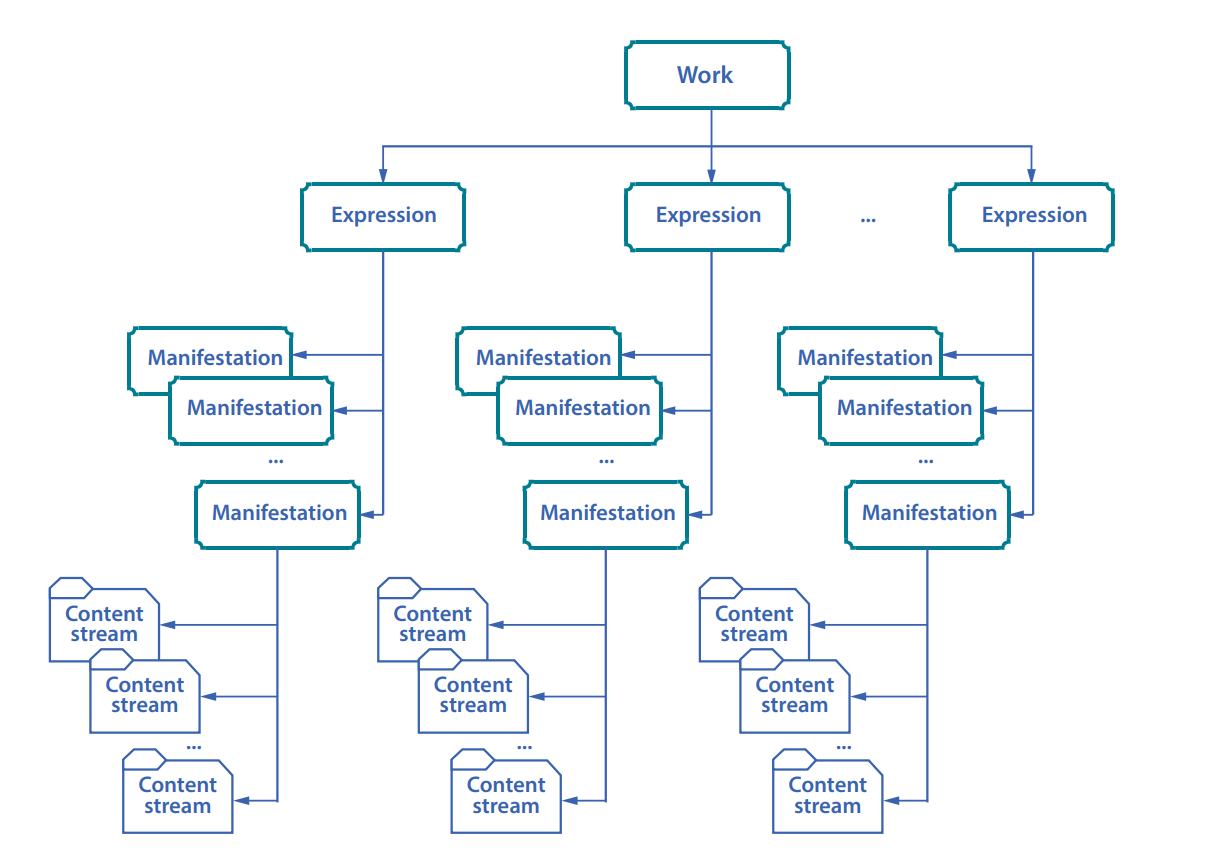
\includegraphics[width=0.75\linewidth]{gfx/content_modell.png}
        \caption{Work-Expresseion-Manifestations-Content Stream Hierarchie}
        \label{fig:eu_wemi}
    \end{figure}
%*************************************************************************
% Other Stuff in the Back
%*************************************************************************
\cleardoublepage%********************************************************************
% Bibliography
%*******************************************************
% work-around to have small caps also here in the headline
% https://tex.stackexchange.com/questions/188126/wrong-header-in-bibliography-classicthesis
% Thanks to Enrico Gregorio
\defbibheading{bibintoc}[\bibname]{%
  \phantomsection
  \manualmark
  \markboth{\spacedlowsmallcaps{#1}}{\spacedlowsmallcaps{#1}}%
  \addtocontents{toc}{\protect\vspace{\beforebibskip}}%
  \addcontentsline{toc}{chapter}{\tocEntry{#1}}%
  \chapter*{#1}%
}
\printbibliography[heading=bibintoc]

%*************************************************************************
% Game Over: Restore, Restart, or Quit?
%*************************************************************************
\end{document}
%*************************************************************************
